\documentclass[twoside]{book}

% Packages required by doxygen
\usepackage{fixltx2e}
\usepackage{calc}
\usepackage{doxygen}
\usepackage[export]{adjustbox} % also loads graphicx
\usepackage{graphicx}
\usepackage[utf8]{inputenc}
\usepackage{makeidx}
\usepackage{multicol}
\usepackage{multirow}
\PassOptionsToPackage{warn}{textcomp}
\usepackage{textcomp}
\usepackage[nointegrals]{wasysym}
\usepackage[table]{xcolor}

% Font selection
\usepackage[T1]{fontenc}
\usepackage[scaled=.90]{helvet}
\usepackage{courier}
\usepackage{amssymb}
\usepackage{sectsty}
\renewcommand{\familydefault}{\sfdefault}
\allsectionsfont{%
  \fontseries{bc}\selectfont%
  \color{darkgray}%
}
\renewcommand{\DoxyLabelFont}{%
  \fontseries{bc}\selectfont%
  \color{darkgray}%
}
\newcommand{\+}{\discretionary{\mbox{\scriptsize$\hookleftarrow$}}{}{}}

% Page & text layout
\usepackage{geometry}
\geometry{%
  a4paper,%
  top=2.5cm,%
  bottom=2.5cm,%
  left=2.5cm,%
  right=2.5cm%
}
\tolerance=750
\hfuzz=15pt
\hbadness=750
\setlength{\emergencystretch}{15pt}
\setlength{\parindent}{0cm}
\setlength{\parskip}{3ex plus 2ex minus 2ex}
\makeatletter
\renewcommand{\paragraph}{%
  \@startsection{paragraph}{4}{0ex}{-1.0ex}{1.0ex}{%
    \normalfont\normalsize\bfseries\SS@parafont%
  }%
}
\renewcommand{\subparagraph}{%
  \@startsection{subparagraph}{5}{0ex}{-1.0ex}{1.0ex}{%
    \normalfont\normalsize\bfseries\SS@subparafont%
  }%
}
\makeatother

% Headers & footers
\usepackage{fancyhdr}
\pagestyle{fancyplain}
\fancyhead[LE]{\fancyplain{}{\bfseries\thepage}}
\fancyhead[CE]{\fancyplain{}{}}
\fancyhead[RE]{\fancyplain{}{\bfseries\leftmark}}
\fancyhead[LO]{\fancyplain{}{\bfseries\rightmark}}
\fancyhead[CO]{\fancyplain{}{}}
\fancyhead[RO]{\fancyplain{}{\bfseries\thepage}}
\fancyfoot[LE]{\fancyplain{}{}}
\fancyfoot[CE]{\fancyplain{}{}}
\fancyfoot[RE]{\fancyplain{}{\bfseries\scriptsize Generated by Doxygen }}
\fancyfoot[LO]{\fancyplain{}{\bfseries\scriptsize Generated by Doxygen }}
\fancyfoot[CO]{\fancyplain{}{}}
\fancyfoot[RO]{\fancyplain{}{}}
\renewcommand{\footrulewidth}{0.4pt}
\renewcommand{\chaptermark}[1]{%
  \markboth{#1}{}%
}
\renewcommand{\sectionmark}[1]{%
  \markright{\thesection\ #1}%
}

% Indices & bibliography
\usepackage{natbib}
\usepackage[titles]{tocloft}
\setcounter{tocdepth}{3}
\setcounter{secnumdepth}{5}
\makeindex

% Hyperlinks (required, but should be loaded last)
\usepackage{ifpdf}
\ifpdf
  \usepackage[pdftex,pagebackref=true]{hyperref}
\else
  \usepackage[ps2pdf,pagebackref=true]{hyperref}
\fi
\hypersetup{%
  colorlinks=true,%
  linkcolor=blue,%
  citecolor=blue,%
  unicode%
}

% Custom commands
\newcommand{\clearemptydoublepage}{%
  \newpage{\pagestyle{empty}\cleardoublepage}%
}

\usepackage{caption}
\captionsetup{labelsep=space,justification=centering,font={bf},singlelinecheck=off,skip=4pt,position=top}

%===== C O N T E N T S =====

\begin{document}

% Titlepage & ToC
\hypersetup{pageanchor=false,
             bookmarksnumbered=true,
             pdfencoding=unicode
            }
\pagenumbering{alph}
\begin{titlepage}
\vspace*{7cm}
\begin{center}%
{\Large Magos Project }\\
\vspace*{1cm}
{\large Generated by Doxygen 1.8.13}\\
\end{center}
\end{titlepage}
\clearemptydoublepage
\pagenumbering{roman}
\tableofcontents
\clearemptydoublepage
\pagenumbering{arabic}
\hypersetup{pageanchor=true}

%--- Begin generated contents ---
\chapter{Magos Index Page}
\label{index}\hypertarget{index}{}\hypertarget{index_intro_sec}{}\section{Introduction}\label{index_intro_sec}
{\bfseries Wellcome to M\+A\+G\+OS Project.} This is a maze genarator solve (M\+A\+G\+OS) Program\+: The magos creates an M\+Aze on canvas build and solve is two way first Backtrack and left hand by your choice.\hypertarget{index_install_sec}{}\section{Run}\label{index_install_sec}
\hypertarget{index_step1}{}\subsection{Step 1\+: Make ./magos}\label{index_step1}
g++ -\/\+Wall -\/std=c++11 \hyperlink{main_8cpp}{src/main.\+cpp} \hyperlink{canvas_8cpp}{src/canvas.\+cpp} \hyperlink{render_8cpp}{src/render.\+cpp} \hyperlink{build_8cpp}{src/build.\+cpp} \hyperlink{solve_8cpp}{src/solve.\+cpp} \hyperlink{game__loop_8cpp}{src/game\+\_\+loop.\+cpp} -\/I include/ -\/o magos\hypertarget{index_step2}{}\subsection{Step 2\+: Run ./magos}\label{index_step2}
Dont forgot rows(2x3), colums(3x2), width(100x100) and height(100x100). ./keno data/bet.\+dat 40, 60, 1200, 800 lower configuration (2x3) or (3x2) and (100x100). On class \hyperlink{classBuild}{Build} you can choose how much map can be random, if the map is to big can take to long time to build because the cell are pick randomly to fix this can set percent random to 40\%.

Left-\/hand \hyperlink{classSolve}{Solve} on this setup the the alway will begin face the north and your left hand on left every time them is not have free pass to front we will turn to clockwise.\hypertarget{index_step3}{}\subsection{Step 3\+: Magos Running}\label{index_step3}
when magos start image will be creates on specific folder.\hypertarget{index_step4}{}\subsection{Step 4\+: Author}\label{index_step4}
\begin{DoxyAuthor}{Author}
Bergony Bandeira
\end{DoxyAuthor}
\begin{DoxyDate}{Date}
05/12/2018 
\end{DoxyDate}

\chapter{Class Index}
\section{Class List}
Here are the classes, structs, unions and interfaces with brief descriptions\+:\begin{DoxyCompactList}
\item\contentsline{section}{\hyperlink{classBuild}{Build} \\*{\bfseries Class} \hyperlink{classBuild}{Build} {\itshape Class that recives a \hyperlink{classMaze}{Maze} to be \hyperlink{classBuild}{Build}.} }{\pageref{classBuild}}{}
\item\contentsline{section}{\hyperlink{classCanvas}{Canvas} \\*{\bfseries Class} \hyperlink{classCanvas}{Canvas} {\itshape Class to creates a \hyperlink{classCanvas}{Canvas} to be draw( Line and Box ).} }{\pageref{classCanvas}}{}
\item\contentsline{section}{\hyperlink{structColor}{Color} \\*{\bfseries Struct} \hyperlink{structColor}{Color} {\itshape  \hyperlink{structColor}{Color} of to printer.} }{\pageref{structColor}}{}
\item\contentsline{section}{\hyperlink{classGame__Loop}{Game\+\_\+\+Loop} \\*{\bfseries Class} Game\+\_\+loop {\itshape Class to control output. input and end of game.} }{\pageref{classGame__Loop}}{}
\item\contentsline{section}{\hyperlink{classMaze}{Maze} \\*{\bfseries Class} \hyperlink{classMaze}{Maze} {\itshape Class create a \hyperlink{classMaze}{Maze} to be \hyperlink{classBuild}{Build}, \hyperlink{classSolve}{Solve} and \hyperlink{classRender}{Render}.} }{\pageref{classMaze}}{}
\item\contentsline{section}{\hyperlink{classRender}{Render} \\*{\bfseries Class} \hyperlink{classRender}{Render} {\itshape A class that recive \hyperlink{classMaze}{Maze} Object to draw in the \hyperlink{classCanvas}{Canvas}.} }{\pageref{classRender}}{}
\item\contentsline{section}{\hyperlink{classSolve}{Solve} \\*{\bfseries Class} \hyperlink{classSolve}{Solve} {\itshape Class that recive a \hyperlink{classMaze}{Maze} to be \hyperlink{classSolve}{Solve}.} }{\pageref{classSolve}}{}
\end{DoxyCompactList}

\chapter{File Index}
\section{File List}
Here is a list of all files with brief descriptions\+:\begin{DoxyCompactList}
\item\contentsline{section}{/home/bergony/lp\+\_\+magos/include/\hyperlink{build_8h}{build.\+h} }{\pageref{build_8h}}{}
\item\contentsline{section}{/home/bergony/lp\+\_\+magos/include/\hyperlink{canvas_8h}{canvas.\+h} }{\pageref{canvas_8h}}{}
\item\contentsline{section}{/home/bergony/lp\+\_\+magos/include/\hyperlink{game__loop_8h}{game\+\_\+loop.\+h} }{\pageref{game__loop_8h}}{}
\item\contentsline{section}{/home/bergony/lp\+\_\+magos/include/\hyperlink{maze_8h}{maze.\+h} }{\pageref{maze_8h}}{}
\item\contentsline{section}{/home/bergony/lp\+\_\+magos/include/\hyperlink{render_8h}{render.\+h} }{\pageref{render_8h}}{}
\item\contentsline{section}{/home/bergony/lp\+\_\+magos/include/\hyperlink{solve_8h}{solve.\+h} }{\pageref{solve_8h}}{}
\item\contentsline{section}{/home/bergony/lp\+\_\+magos/src/\hyperlink{build_8cpp}{build.\+cpp} }{\pageref{build_8cpp}}{}
\item\contentsline{section}{/home/bergony/lp\+\_\+magos/src/\hyperlink{canvas_8cpp}{canvas.\+cpp} }{\pageref{canvas_8cpp}}{}
\item\contentsline{section}{/home/bergony/lp\+\_\+magos/src/\hyperlink{game__loop_8cpp}{game\+\_\+loop.\+cpp} }{\pageref{game__loop_8cpp}}{}
\item\contentsline{section}{/home/bergony/lp\+\_\+magos/src/\hyperlink{main_8cpp}{main.\+cpp} }{\pageref{main_8cpp}}{}
\item\contentsline{section}{/home/bergony/lp\+\_\+magos/src/\hyperlink{maze_8cpp}{maze.\+cpp} }{\pageref{maze_8cpp}}{}
\item\contentsline{section}{/home/bergony/lp\+\_\+magos/src/\hyperlink{render_8cpp}{render.\+cpp} }{\pageref{render_8cpp}}{}
\item\contentsline{section}{/home/bergony/lp\+\_\+magos/src/\hyperlink{solve_8cpp}{solve.\+cpp} }{\pageref{solve_8cpp}}{}
\end{DoxyCompactList}

\chapter{Class Documentation}
\hypertarget{classBuild}{}\section{Build Class Reference}
\label{classBuild}\index{Build@{Build}}


{\bfseries Class} \hyperlink{classBuild}{Build} {\itshape Class that recives a \hyperlink{classMaze}{Maze} to be \hyperlink{classBuild}{Build}.}  




{\ttfamily \#include $<$build.\+h$>$}

\subsection*{Public Member Functions}
\begin{DoxyCompactItemize}
\item 
\hyperlink{classBuild_a1b8365d07d8ab0c0d107fbc30ee6eb1c}{Build} (\hyperlink{classMaze}{Maze} $\ast$m)
\begin{DoxyCompactList}\small\item\em ! Constructor \hyperlink{classBuild}{Build} \end{DoxyCompactList}\item 
\hyperlink{classBuild_a96ad56fb129cfbc2131fd094c41ae1ec}{Build} ()
\begin{DoxyCompactList}\small\item\em ! Constructor \hyperlink{classBuild}{Build} Default \end{DoxyCompactList}\item 
\hyperlink{classBuild_a7fc2f29804f9dc29b640838b515841e8}{$\sim$\+Build} (void)
\begin{DoxyCompactList}\small\item\em ! Destructors \hyperlink{classBuild}{Build}. \end{DoxyCompactList}\item 
\hyperlink{classBuild_aeadb5e6bafcfb4e7811bbd434ac5c663}{Build} (const \hyperlink{classBuild}{Build} \&clone)
\begin{DoxyCompactList}\small\item\em ! Copy \hyperlink{classBuild}{Build}. \end{DoxyCompactList}\item 
\hyperlink{classBuild}{Build} \& \hyperlink{classBuild_a72dbb04928303d0b90d003cb90d85550}{operator=} (const \hyperlink{classBuild}{Build} \&b)
\begin{DoxyCompactList}\small\item\em ! Assignment operator. \end{DoxyCompactList}\item 
bool \hyperlink{classBuild_a72373ff38b0676c8f2c9f171c15333c4}{done} (void)
\begin{DoxyCompactList}\small\item\em Method to check if the \hyperlink{classMaze}{Maze} is done on \hyperlink{classBuild}{Build}. \end{DoxyCompactList}\item 
bool \hyperlink{classBuild_ada5111f265ee6a43832db25e8da9c3d0}{make} (void)
\begin{DoxyCompactList}\small\item\em Method add Cell to lab. \end{DoxyCompactList}\item 
bool \hyperlink{classBuild_ae4eeedfd95306c08d50aff3f620b5a47}{is\+\_\+on\+\_\+set} (int s1, int s2)
\begin{DoxyCompactList}\small\item\em Method to check if two set is already in the same set. \end{DoxyCompactList}\item 
void \hyperlink{classBuild_af1582ef11fb92698ba75581f2f7ead02}{union\+\_\+sets} (int s1, int s2)
\begin{DoxyCompactList}\small\item\em Method Union to two set and them sub-\/set. \end{DoxyCompactList}\end{DoxyCompactItemize}


\subsection{Detailed Description}
{\bfseries Class} \hyperlink{classBuild}{Build} {\itshape Class that recives a \hyperlink{classMaze}{Maze} to be \hyperlink{classBuild}{Build}.} 

\subsection{Constructor \& Destructor Documentation}
\mbox{\Hypertarget{classBuild_a1b8365d07d8ab0c0d107fbc30ee6eb1c}\label{classBuild_a1b8365d07d8ab0c0d107fbc30ee6eb1c}} 
\index{Build@{Build}!Build@{Build}}
\index{Build@{Build}!Build@{Build}}
\subsubsection{\texorpdfstring{Build()}{Build()}\hspace{0.1cm}{\footnotesize\ttfamily [1/3]}}
{\footnotesize\ttfamily Build\+::\+Build (\begin{DoxyParamCaption}\item[{\hyperlink{classMaze}{Maze} $\ast$}]{m }\end{DoxyParamCaption})\hspace{0.3cm}{\ttfamily [inline]}}



! Constructor \hyperlink{classBuild}{Build} 


\begin{DoxyParams}{Parameters}
{\em \hyperlink{classMaze}{Maze}} & $\ast$m Referece to a \hyperlink{classMaze}{Maze}. \\
\hline
\end{DoxyParams}
$<$Change size of vector fill a All cell.

$<$ Creates a set of Cell.

$<$ Add a cell to to set.

$<$ Add Set to Vector. 
\begin{DoxyCode}
23                         : m\_maze\{m\}
24         \{
25             m\_sets\_cell.resize(m\_maze->\hyperlink{classMaze_a90f5c1c140a9991942204d4a7fec3bf8}{get\_numb\_cell}());        
26 
27             \textcolor{keywordflow}{for}(\textcolor{keywordtype}{int} i\{0\}; i < m\_maze->\hyperlink{classMaze_a90f5c1c140a9991942204d4a7fec3bf8}{get\_numb\_cell}(); i++)
28             \{
29                 std::set< int > my\_set;     
30                 my\_set.insert(i);           
31                 m\_sets\_cell[i] = my\_set;    
32             \}
33         \}
\end{DoxyCode}
Here is the call graph for this function\+:\nopagebreak
\begin{figure}[H]
\begin{center}
\leavevmode
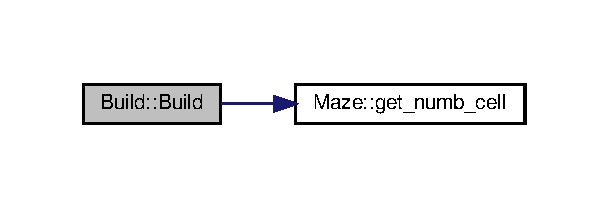
\includegraphics[width=292pt]{classBuild_a1b8365d07d8ab0c0d107fbc30ee6eb1c_cgraph}
\end{center}
\end{figure}
\mbox{\Hypertarget{classBuild_a96ad56fb129cfbc2131fd094c41ae1ec}\label{classBuild_a96ad56fb129cfbc2131fd094c41ae1ec}} 
\index{Build@{Build}!Build@{Build}}
\index{Build@{Build}!Build@{Build}}
\subsubsection{\texorpdfstring{Build()}{Build()}\hspace{0.1cm}{\footnotesize\ttfamily [2/3]}}
{\footnotesize\ttfamily Build\+::\+Build (\begin{DoxyParamCaption}{ }\end{DoxyParamCaption})\hspace{0.3cm}{\ttfamily [inline]}}



! Constructor \hyperlink{classBuild}{Build} Default 


\begin{DoxyCode}
36 \{\}
\end{DoxyCode}
\mbox{\Hypertarget{classBuild_a7fc2f29804f9dc29b640838b515841e8}\label{classBuild_a7fc2f29804f9dc29b640838b515841e8}} 
\index{Build@{Build}!````~Build@{$\sim$\+Build}}
\index{````~Build@{$\sim$\+Build}!Build@{Build}}
\subsubsection{\texorpdfstring{$\sim$\+Build()}{~Build()}}
{\footnotesize\ttfamily Build\+::$\sim$\+Build (\begin{DoxyParamCaption}\item[{void}]{ }\end{DoxyParamCaption})\hspace{0.3cm}{\ttfamily [inline]}}



! Destructors \hyperlink{classBuild}{Build}. 


\begin{DoxyCode}
39         \{
40             \textcolor{comment}{/*EMPTY*/}
41         \}
\end{DoxyCode}
\mbox{\Hypertarget{classBuild_aeadb5e6bafcfb4e7811bbd434ac5c663}\label{classBuild_aeadb5e6bafcfb4e7811bbd434ac5c663}} 
\index{Build@{Build}!Build@{Build}}
\index{Build@{Build}!Build@{Build}}
\subsubsection{\texorpdfstring{Build()}{Build()}\hspace{0.1cm}{\footnotesize\ttfamily [3/3]}}
{\footnotesize\ttfamily Build\+::\+Build (\begin{DoxyParamCaption}\item[{const \hyperlink{classBuild}{Build} \&}]{clone }\end{DoxyParamCaption})\hspace{0.3cm}{\ttfamily [inline]}}



! Copy \hyperlink{classBuild}{Build}. 


\begin{DoxyCode}
45         \{
46             m\_maze = clone.m\_maze;
47             m\_sets\_cell = clone.m\_sets\_cell;
48             m\_set\_done = clone.m\_set\_done;
49         \}
\end{DoxyCode}


\subsection{Member Function Documentation}
\mbox{\Hypertarget{classBuild_a72373ff38b0676c8f2c9f171c15333c4}\label{classBuild_a72373ff38b0676c8f2c9f171c15333c4}} 
\index{Build@{Build}!done@{done}}
\index{done@{done}!Build@{Build}}
\subsubsection{\texorpdfstring{done()}{done()}}
{\footnotesize\ttfamily bool Build\+::done (\begin{DoxyParamCaption}\item[{void}]{ }\end{DoxyParamCaption})}



Method to check if the \hyperlink{classMaze}{Maze} is done on \hyperlink{classBuild}{Build}. 

\begin{DoxyReturn}{Returns}
True a set is on the same set otherwise False. 
\end{DoxyReturn}

\begin{DoxyCode}
6 \{
7     \textcolor{keywordflow}{if}(m\_set\_done ==  (m\_maze->\hyperlink{classMaze_a90f5c1c140a9991942204d4a7fec3bf8}{get\_numb\_cell}()-1) )
8     \{
9         \textcolor{keywordflow}{return} \textcolor{keyword}{true};
10     \}
11 
12     \textcolor{keywordflow}{return} \textcolor{keyword}{false};
13 \}
\end{DoxyCode}
Here is the call graph for this function\+:\nopagebreak
\begin{figure}[H]
\begin{center}
\leavevmode
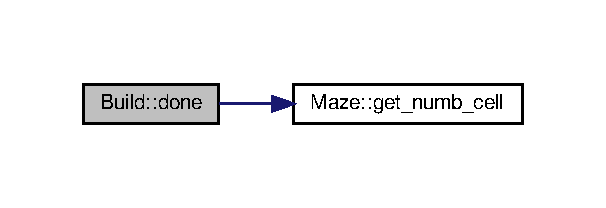
\includegraphics[width=291pt]{classBuild_a72373ff38b0676c8f2c9f171c15333c4_cgraph}
\end{center}
\end{figure}
Here is the caller graph for this function\+:\nopagebreak
\begin{figure}[H]
\begin{center}
\leavevmode
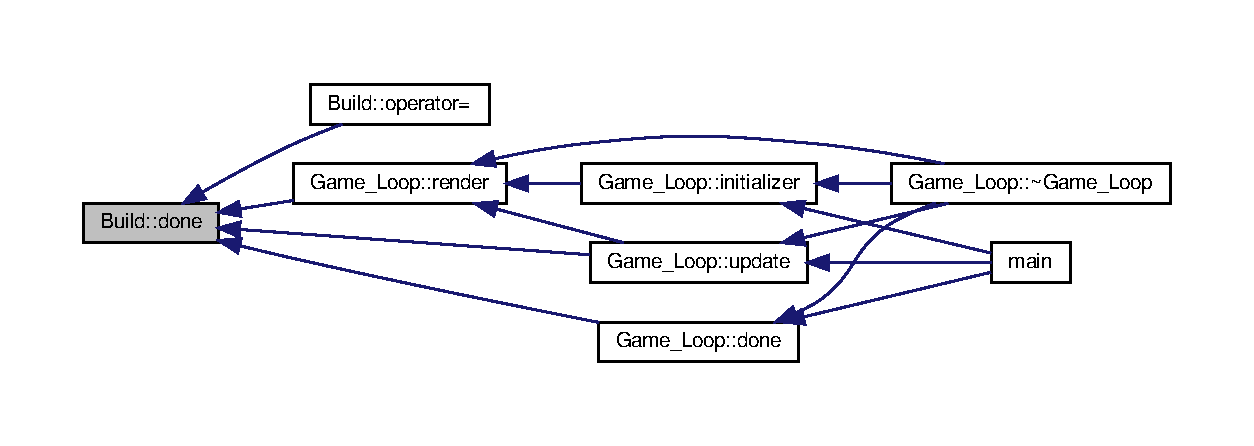
\includegraphics[width=350pt]{classBuild_a72373ff38b0676c8f2c9f171c15333c4_icgraph}
\end{center}
\end{figure}
\mbox{\Hypertarget{classBuild_ae4eeedfd95306c08d50aff3f620b5a47}\label{classBuild_ae4eeedfd95306c08d50aff3f620b5a47}} 
\index{Build@{Build}!is\+\_\+on\+\_\+set@{is\+\_\+on\+\_\+set}}
\index{is\+\_\+on\+\_\+set@{is\+\_\+on\+\_\+set}!Build@{Build}}
\subsubsection{\texorpdfstring{is\+\_\+on\+\_\+set()}{is\_on\_set()}}
{\footnotesize\ttfamily bool Build\+::is\+\_\+on\+\_\+set (\begin{DoxyParamCaption}\item[{int}]{s1,  }\item[{int}]{s2 }\end{DoxyParamCaption})}



Method to check if two set is already in the same set. 


\begin{DoxyParams}{Parameters}
{\em int} & s1 First set. \\
\hline
{\em int} & s2 Secontd Set. \\
\hline
\end{DoxyParams}
\begin{DoxyReturn}{Returns}
True if s1 is on s2 otherwise False. 
\end{DoxyReturn}

\begin{DoxyCode}
45 \{
46     \textcolor{comment}{//Check the first SET}
47     \textcolor{keywordflow}{for}(std::set<int>::iterator it\_s1 = m\_sets\_cell[s1].begin(); 
48             it\_s1 != m\_sets\_cell[s1].end(); it\_s1++)
49     \{
50         \textcolor{keywordflow}{for}(std::set<int>::iterator it\_s2 = m\_sets\_cell[s2].begin(); 
51                 it\_s2 != m\_sets\_cell[s2].end(); it\_s2++)
52         \{
53             \textcolor{keywordflow}{if}( m\_sets\_cell[*it\_s1].count(*it\_s2) )
54             \{
55                 \textcolor{keywordflow}{return} \textcolor{keyword}{true};
56             \}
57         \}
58     \}
59     \textcolor{comment}{//Check the Second Set}
60     \textcolor{keywordflow}{for}(std::set<int>::iterator it\_s2 = m\_sets\_cell[s2].begin(); 
61             it\_s2 != m\_sets\_cell[s2].end(); it\_s2++)
62     \{
63         \textcolor{keywordflow}{for}(std::set<int>::iterator it\_s1 = m\_sets\_cell[s1].begin(); 
64                 it\_s1 != m\_sets\_cell[s1].end(); it\_s1++)
65 
66         \{
67             \textcolor{keywordflow}{if}( m\_sets\_cell[*it\_s2].count(*it\_s1) )
68             \{
69                 \textcolor{keywordflow}{return} \textcolor{keyword}{true};
70             \}
71         \}
72     \}
73 
74     \textcolor{keywordflow}{return} \textcolor{keyword}{false};
75 
76 \}
\end{DoxyCode}
Here is the caller graph for this function\+:\nopagebreak
\begin{figure}[H]
\begin{center}
\leavevmode
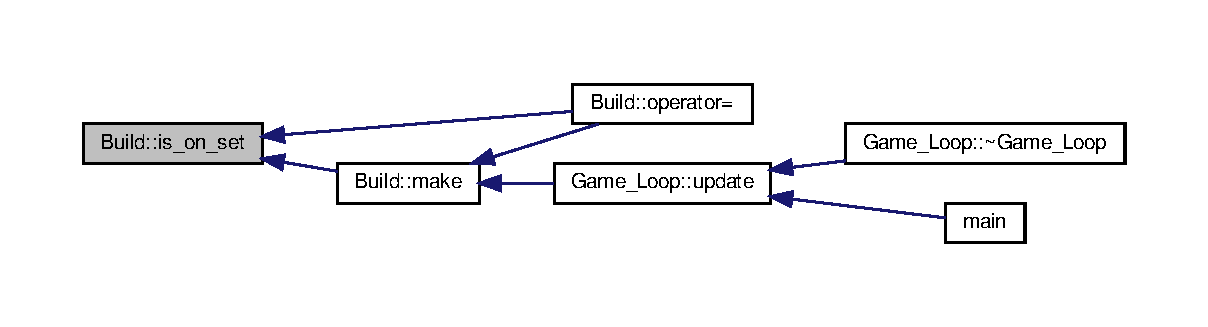
\includegraphics[width=350pt]{classBuild_ae4eeedfd95306c08d50aff3f620b5a47_icgraph}
\end{center}
\end{figure}
\mbox{\Hypertarget{classBuild_ada5111f265ee6a43832db25e8da9c3d0}\label{classBuild_ada5111f265ee6a43832db25e8da9c3d0}} 
\index{Build@{Build}!make@{make}}
\index{make@{make}!Build@{Build}}
\subsubsection{\texorpdfstring{make()}{make()}}
{\footnotesize\ttfamily bool Build\+::make (\begin{DoxyParamCaption}\item[{void}]{ }\end{DoxyParamCaption})}



Method add Cell to lab. 

\begin{DoxyReturn}{Returns}
True if cell is add otherwise False. 
\end{DoxyReturn}
$<$ Change send

$<$ Coordinates Y

$<$ Coordinates X

$<$ Cell to be add.

$<$ Cell set

$<$ Percent of the random \hyperlink{classMaze}{Maze}

$<$ valor to The wall to be random. 
\begin{DoxyCode}
79 \{
80     srand(time(NULL));  
81     \textcolor{keywordtype}{int} y\{0\};           
82     \textcolor{keywordtype}{int} x\{0\};           
83     \textcolor{keywordtype}{int} i\{0\};           
84     \textcolor{keywordtype}{int} look\_cell\{0\};   
85     \textcolor{keywordtype}{int} percent\{0\};     
86     \textcolor{keywordtype}{int} number\_of\_percent\{100\};
87     \textcolor{keywordtype}{int} rand\_wall\{0\};   
88 
89     percent = (m\_maze->\hyperlink{classMaze_a90f5c1c140a9991942204d4a7fec3bf8}{get\_numb\_cell}() * number\_of\_percent) / 100;
90     rand\_wall = rand() % 3;
91 
92     \textcolor{keywordflow}{if}( m\_set\_done < percent)
93     \{
94         y = rand() % (m\_maze->\hyperlink{classMaze_ac786606a34632b2254b2d27d5f5f0f3f}{get\_rows}());
95         x = rand() % (m\_maze->\hyperlink{classMaze_a8a04cd1335e96a80358181afa164d4c9}{get\_cols}());
96         i = m\_maze->\hyperlink{classMaze_aa59b935dcd5f7129636cea6e40882c56}{find\_cell}(x , y);
97     \}
98     \textcolor{keywordflow}{else}
99     \{
100         \textcolor{keywordflow}{for}(\textcolor{keywordtype}{int} cell\_out\{0\} ; cell\_out < m\_maze->\hyperlink{classMaze_a90f5c1c140a9991942204d4a7fec3bf8}{get\_numb\_cell}(); cell\_out++)
101         \{
102             \textcolor{keywordflow}{while}(m\_sets\_cell[look\_cell].size() > (\textcolor{keywordtype}{unsigned} int)(m\_maze->
      \hyperlink{classMaze_a90f5c1c140a9991942204d4a7fec3bf8}{get\_numb\_cell}()-1) )
103             \{   
104                 look\_cell++;
105                 x=0;
106                 y=0;
107             \}
108             \textcolor{keywordflow}{if}( !\hyperlink{classBuild_ae4eeedfd95306c08d50aff3f620b5a47}{is\_on\_set}(cell\_out, look\_cell))
109             \{
110                 i = cell\_out;
111                 \textcolor{keywordflow}{break};
112             \}
113 
114             x++;
115 
116             \textcolor{keywordflow}{if}(x >= m\_maze->\hyperlink{classMaze_a8a04cd1335e96a80358181afa164d4c9}{get\_cols}())
117             \{
118                 x = 0;
119                 y++;
120             \}
121 
122             look\_cell = 0;
123         \}
124     \}
125 
126     \textcolor{keywordflow}{if}( rand\_wall == 0 && y != 0 && !\hyperlink{classBuild_ae4eeedfd95306c08d50aff3f620b5a47}{is\_on\_set}( i, i-m\_maze->\hyperlink{classMaze_a8a04cd1335e96a80358181afa164d4c9}{get\_cols}() ) )
127     \{
128         \hyperlink{classBuild_af1582ef11fb92698ba75581f2f7ead02}{union\_sets}(i, i-m\_maze->\hyperlink{classMaze_a8a04cd1335e96a80358181afa164d4c9}{get\_cols}());
129         m\_maze->\hyperlink{classMaze_ab86292a84aa56a26c4c07f4aa684d9bb}{set\_cell\_down}(y , x, \hyperlink{classMaze_a07167e321eac2b67100fb82ecb98f1d1ab28354b543375bfa94dabaeda722927f}{Maze::status\_cell::top});
130         m\_maze->\hyperlink{classMaze_ab86292a84aa56a26c4c07f4aa684d9bb}{set\_cell\_down}(y-1 , x, \hyperlink{classMaze_a07167e321eac2b67100fb82ecb98f1d1a74e8333ad11685ff3bdae589c8f6e34d}{Maze::status\_cell::down});
131         m\_set\_done++;
132         \textcolor{keywordflow}{return} \textcolor{keyword}{true};
133     \}
134     \textcolor{keywordflow}{else} \textcolor{keywordflow}{if}( rand\_wall == 1 && x != 0 && !\hyperlink{classBuild_ae4eeedfd95306c08d50aff3f620b5a47}{is\_on\_set}(i , i-1  ))
135     \{
136         \hyperlink{classBuild_af1582ef11fb92698ba75581f2f7ead02}{union\_sets}(i, i-1);
137         m\_maze->\hyperlink{classMaze_ab86292a84aa56a26c4c07f4aa684d9bb}{set\_cell\_down}(y , x, \hyperlink{classMaze_a07167e321eac2b67100fb82ecb98f1d1a811882fecd5c7618d7099ebbd39ea254}{Maze::status\_cell::left});
138         m\_maze->\hyperlink{classMaze_ab86292a84aa56a26c4c07f4aa684d9bb}{set\_cell\_down}(y , x-1, \hyperlink{classMaze_a07167e321eac2b67100fb82ecb98f1d1a7c4f29407893c334a6cb7a87bf045c0d}{Maze::status\_cell::right});
139         m\_set\_done++;
140         \textcolor{keywordflow}{return} \textcolor{keyword}{true};
141     \}
142     \textcolor{keywordflow}{else} \textcolor{keywordflow}{if}( rand\_wall == 2 && y != (m\_maze->\hyperlink{classMaze_ac786606a34632b2254b2d27d5f5f0f3f}{get\_rows}()-1) && !\hyperlink{classBuild_ae4eeedfd95306c08d50aff3f620b5a47}{is\_on\_set}( i, i+m\_maze->
      \hyperlink{classMaze_a8a04cd1335e96a80358181afa164d4c9}{get\_cols}()))
143     \{
144         \hyperlink{classBuild_af1582ef11fb92698ba75581f2f7ead02}{union\_sets}(i, i+m\_maze->\hyperlink{classMaze_a8a04cd1335e96a80358181afa164d4c9}{get\_cols}());
145         m\_maze->\hyperlink{classMaze_ab86292a84aa56a26c4c07f4aa684d9bb}{set\_cell\_down}(y , x, \hyperlink{classMaze_a07167e321eac2b67100fb82ecb98f1d1a74e8333ad11685ff3bdae589c8f6e34d}{Maze::status\_cell::down});
146         m\_maze->\hyperlink{classMaze_ab86292a84aa56a26c4c07f4aa684d9bb}{set\_cell\_down}(y+1 , x, \hyperlink{classMaze_a07167e321eac2b67100fb82ecb98f1d1ab28354b543375bfa94dabaeda722927f}{Maze::status\_cell::top});
147         m\_set\_done++;
148         \textcolor{keywordflow}{return} \textcolor{keyword}{true};
149     \}
150     \textcolor{keywordflow}{else} \textcolor{keywordflow}{if}(rand\_wall == 3 && x != (m\_maze->\hyperlink{classMaze_ac786606a34632b2254b2d27d5f5f0f3f}{get\_rows}()-1) && !\hyperlink{classBuild_ae4eeedfd95306c08d50aff3f620b5a47}{is\_on\_set}( i, i+1 ) )
151     \{
152         \hyperlink{classBuild_af1582ef11fb92698ba75581f2f7ead02}{union\_sets}(i, i+1);
153         m\_maze->\hyperlink{classMaze_ab86292a84aa56a26c4c07f4aa684d9bb}{set\_cell\_down}(y , x, \hyperlink{classMaze_a07167e321eac2b67100fb82ecb98f1d1a7c4f29407893c334a6cb7a87bf045c0d}{Maze::status\_cell::right});
154         m\_maze->\hyperlink{classMaze_ab86292a84aa56a26c4c07f4aa684d9bb}{set\_cell\_down}(y , x+1, \hyperlink{classMaze_a07167e321eac2b67100fb82ecb98f1d1a811882fecd5c7618d7099ebbd39ea254}{Maze::status\_cell::left});
155         m\_set\_done++;
156         \textcolor{keywordflow}{return} \textcolor{keyword}{true};
157     \}
158 
159     \textcolor{keywordflow}{return} \textcolor{keyword}{false};
160 \}
\end{DoxyCode}
Here is the call graph for this function\+:\nopagebreak
\begin{figure}[H]
\begin{center}
\leavevmode
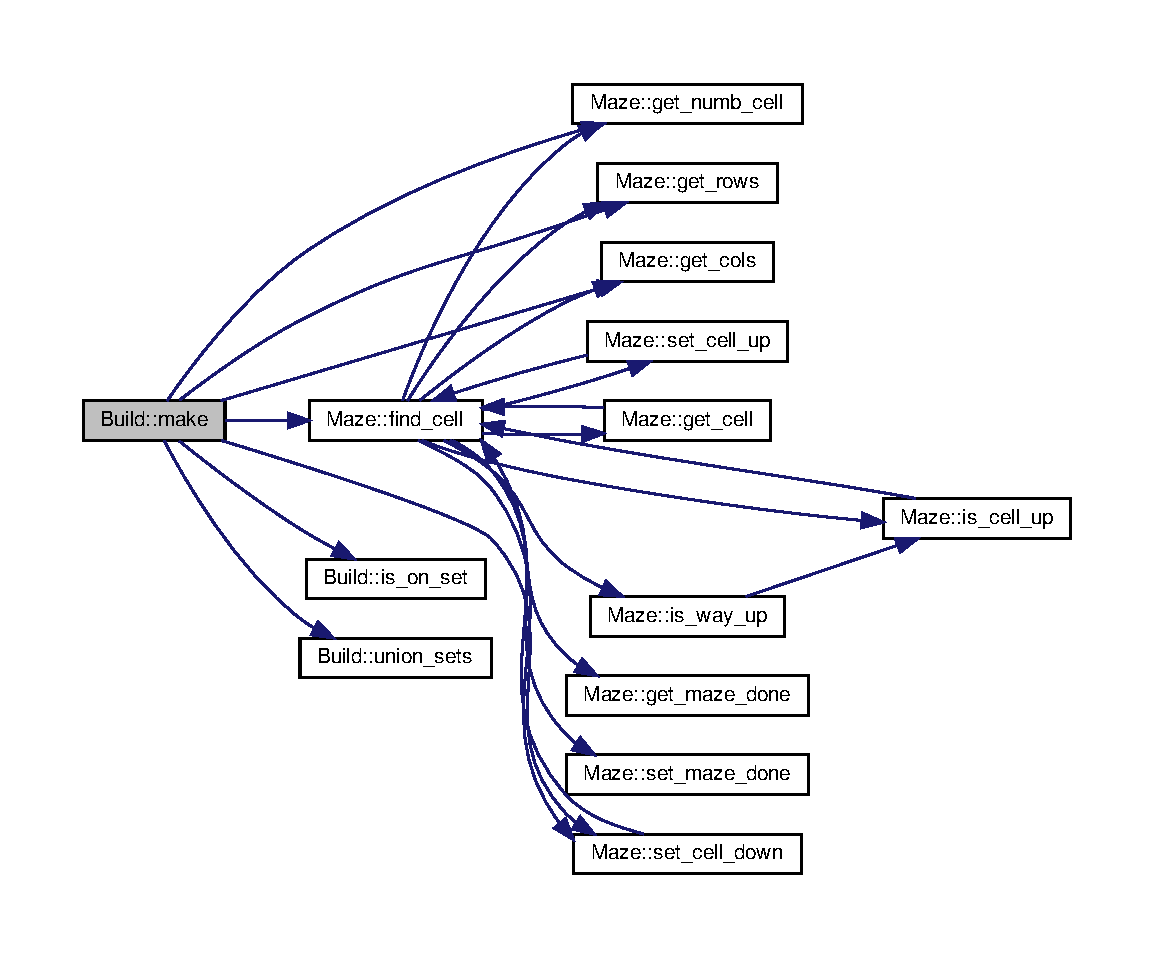
\includegraphics[width=350pt]{classBuild_ada5111f265ee6a43832db25e8da9c3d0_cgraph}
\end{center}
\end{figure}
Here is the caller graph for this function\+:\nopagebreak
\begin{figure}[H]
\begin{center}
\leavevmode
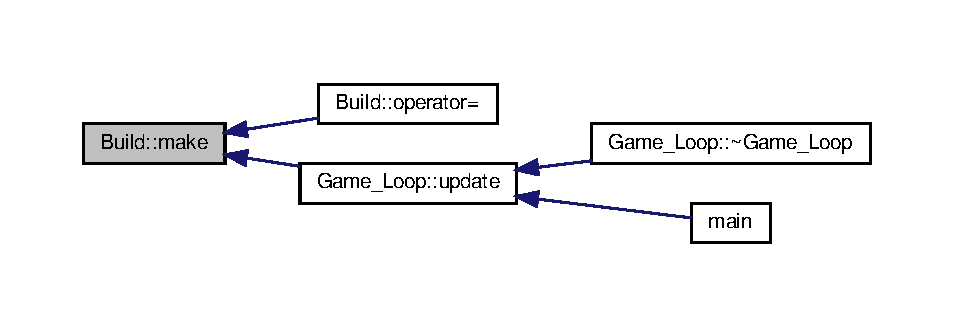
\includegraphics[width=350pt]{classBuild_ada5111f265ee6a43832db25e8da9c3d0_icgraph}
\end{center}
\end{figure}
\mbox{\Hypertarget{classBuild_a72dbb04928303d0b90d003cb90d85550}\label{classBuild_a72dbb04928303d0b90d003cb90d85550}} 
\index{Build@{Build}!operator=@{operator=}}
\index{operator=@{operator=}!Build@{Build}}
\subsubsection{\texorpdfstring{operator=()}{operator=()}}
{\footnotesize\ttfamily \hyperlink{classBuild}{Build}\& Build\+::operator= (\begin{DoxyParamCaption}\item[{const \hyperlink{classBuild}{Build} \&}]{b }\end{DoxyParamCaption})\hspace{0.3cm}{\ttfamily [inline]}}



! Assignment operator. 


\begin{DoxyCode}
53         \{
54             this->m\_maze = b.m\_maze;
55             this->m\_sets\_cell = b.m\_sets\_cell;
56             this->m\_set\_done = b.m\_set\_done;
57 
58             \textcolor{keywordflow}{return} *\textcolor{keyword}{this};
59         \}
\end{DoxyCode}
Here is the call graph for this function\+:\nopagebreak
\begin{figure}[H]
\begin{center}
\leavevmode
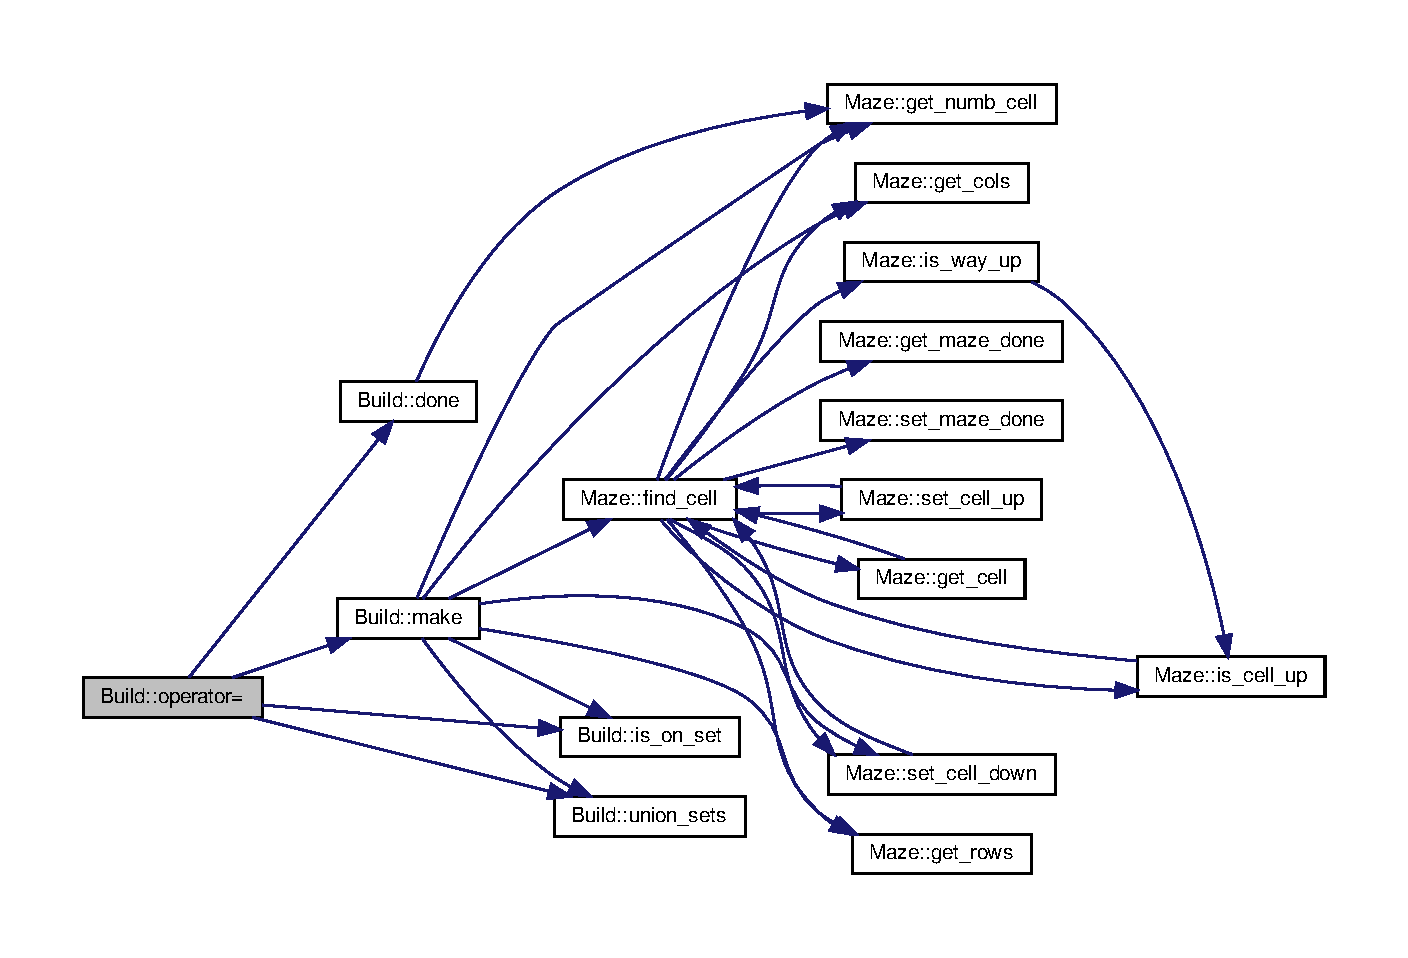
\includegraphics[width=350pt]{classBuild_a72dbb04928303d0b90d003cb90d85550_cgraph}
\end{center}
\end{figure}
\mbox{\Hypertarget{classBuild_af1582ef11fb92698ba75581f2f7ead02}\label{classBuild_af1582ef11fb92698ba75581f2f7ead02}} 
\index{Build@{Build}!union\+\_\+sets@{union\+\_\+sets}}
\index{union\+\_\+sets@{union\+\_\+sets}!Build@{Build}}
\subsubsection{\texorpdfstring{union\+\_\+sets()}{union\_sets()}}
{\footnotesize\ttfamily void Build\+::union\+\_\+sets (\begin{DoxyParamCaption}\item[{int}]{s1,  }\item[{int}]{s2 }\end{DoxyParamCaption})}



Method Union to two set and them sub-\/set. 

int s1 set to be union. 
\begin{DoxyParams}{Parameters}
{\em int} & s2 set to be union. \\
\hline
\end{DoxyParams}

\begin{DoxyCode}
16 \{
17     \textcolor{comment}{//Add on fisrt set}
18     \textcolor{keywordflow}{for}(std::set<int>::iterator it\_s1 = m\_sets\_cell[s1].begin(); 
19             it\_s1 != m\_sets\_cell[s1].end(); it\_s1++)
20     \{
21         \textcolor{keywordflow}{for}(std::set<int>::iterator it\_s2 = m\_sets\_cell[s2].begin(); 
22                 it\_s2 != m\_sets\_cell[s2].end(); it\_s2++)
23         \{
24             \textcolor{keywordflow}{if}( !m\_sets\_cell[*it\_s1].count(*it\_s2) )
25             \{
26                 m\_sets\_cell[*it\_s1].insert(*it\_s2);
27             \}
28         \}
29     \}
30     \textcolor{comment}{//ADd on second set.}
31     \textcolor{keywordflow}{for}(std::set<int>::iterator it\_s2 = m\_sets\_cell[s2].begin(); 
32             it\_s2 != m\_sets\_cell[s2].end(); it\_s2++)
33     \{
34         \textcolor{keywordflow}{for}(std::set<int>::iterator it\_s1 = m\_sets\_cell[s1].begin(); 
35                 it\_s1 != m\_sets\_cell[s1].end(); it\_s1++)
36         \{
37             \textcolor{keywordflow}{if}( !m\_sets\_cell[*it\_s2].count(*it\_s1) )
38             \{
39                 m\_sets\_cell[*it\_s2].insert(*it\_s1);
40             \}
41         \}
42     \}
43 \}
\end{DoxyCode}
Here is the caller graph for this function\+:\nopagebreak
\begin{figure}[H]
\begin{center}
\leavevmode
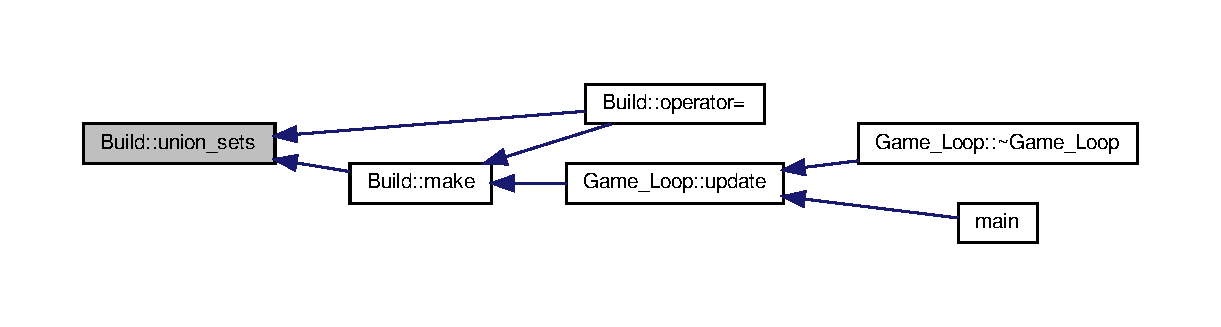
\includegraphics[width=350pt]{classBuild_af1582ef11fb92698ba75581f2f7ead02_icgraph}
\end{center}
\end{figure}


The documentation for this class was generated from the following files\+:\begin{DoxyCompactItemize}
\item 
/home/bergony/lp\+\_\+magos/include/\hyperlink{build_8h}{build.\+h}\item 
/home/bergony/lp\+\_\+magos/src/\hyperlink{build_8cpp}{build.\+cpp}\end{DoxyCompactItemize}

\hypertarget{classCanvas}{}\section{Canvas Class Reference}
\label{classCanvas}\index{Canvas@{Canvas}}


{\bfseries Class} \hyperlink{classCanvas}{Canvas} {\itshape Class to creates a \hyperlink{classCanvas}{Canvas} to be draw( Line and Box ).}  




{\ttfamily \#include $<$canvas.\+h$>$}

\subsection*{Public Member Functions}
\begin{DoxyCompactItemize}
\item 
\hyperlink{classCanvas_aa232b6ded8df451736a9e042e103c4e2}{Canvas} (int w=0, int h=0)
\begin{DoxyCompactList}\small\item\em ! Constructor \hyperlink{classCanvas}{Canvas} \end{DoxyCompactList}\item 
\hyperlink{classCanvas_a63c450c44bae6e3ff76a07ad0a15a750}{$\sim$\+Canvas} (void)
\begin{DoxyCompactList}\small\item\em ! Destructors \hyperlink{classCanvas}{Canvas} \end{DoxyCompactList}\item 
\hyperlink{classCanvas_afcffecf500f90749912bfe626eba9acc}{Canvas} (const \hyperlink{classCanvas}{Canvas} \&clone)
\begin{DoxyCompactList}\small\item\em ! Copy \hyperlink{classCanvas}{Canvas}. \end{DoxyCompactList}\item 
\hyperlink{classCanvas}{Canvas} \& \hyperlink{classCanvas_a2b44607cedf966c39c1e7c2b4abcb880}{operator=} (const \hyperlink{classCanvas}{Canvas} \&c)
\begin{DoxyCompactList}\small\item\em ! Assignment operator. \end{DoxyCompactList}\item 
int \hyperlink{classCanvas_a8478392f133ddaf1c9b7272a301c7898}{get\+\_\+w} (void) const
\begin{DoxyCompactList}\small\item\em Method to get width of the \hyperlink{classCanvas}{Canvas}. \end{DoxyCompactList}\item 
int \hyperlink{classCanvas_ab26c7ab91a0a9069895285a314bc8418}{get\+\_\+h} (void) const
\begin{DoxyCompactList}\small\item\em Method to get height of the \hyperlink{classCanvas}{Canvas}. \end{DoxyCompactList}\item 
\hyperlink{canvas_8h_a0c8186d9b9b7880309c27230bbb5e69d}{byte} $\ast$ \hyperlink{classCanvas_aa9f9b173d57058ea827a0134c937d0e1}{get\+\_\+p} (void) const
\begin{DoxyCompactList}\small\item\em Method to get the Point of the begin \hyperlink{classCanvas}{Canvas}. \end{DoxyCompactList}\item 
void \hyperlink{classCanvas_a0205269b201aed71f21b8f613cd66333}{clear} (\hyperlink{structColor}{Color} color)
\begin{DoxyCompactList}\small\item\em Printer the full \hyperlink{classCanvas}{Canvas} with a \hyperlink{structColor}{Color} param. \end{DoxyCompactList}\item 
void \hyperlink{classCanvas_a3095d5ff2670c5dc9939454198865ceb}{hline} (const int \&x, const int \&y, const int \&w, \hyperlink{structColor}{Color} color)
\begin{DoxyCompactList}\small\item\em Printer a Horizontal line. \end{DoxyCompactList}\item 
void \hyperlink{classCanvas_af81ae19142bc132665e053ce5de15211}{vline} (const int \&x, const int \&y, const int \&h, \hyperlink{structColor}{Color} color)
\begin{DoxyCompactList}\small\item\em Printer a Vertical line. \end{DoxyCompactList}\item 
void \hyperlink{classCanvas_a6e1c6baa6fb92cd3de1726b67b51aa38}{box} (const int \&x, const int \&y, const int \&w, const int \&h, \hyperlink{structColor}{Color} color)
\begin{DoxyCompactList}\small\item\em Printer a Box. \end{DoxyCompactList}\item 
void \hyperlink{classCanvas_aa189a705135fb14f427747084763143a}{pixel} (const int \&x, const int \&y, \hyperlink{structColor}{Color} color)
\begin{DoxyCompactList}\small\item\em Printer a single pixel on canvs. \end{DoxyCompactList}\end{DoxyCompactItemize}


\subsection{Detailed Description}
{\bfseries Class} \hyperlink{classCanvas}{Canvas} {\itshape Class to creates a \hyperlink{classCanvas}{Canvas} to be draw( Line and Box ).} 

\subsection{Constructor \& Destructor Documentation}
\mbox{\Hypertarget{classCanvas_aa232b6ded8df451736a9e042e103c4e2}\label{classCanvas_aa232b6ded8df451736a9e042e103c4e2}} 
\index{Canvas@{Canvas}!Canvas@{Canvas}}
\index{Canvas@{Canvas}!Canvas@{Canvas}}
\subsubsection{\texorpdfstring{Canvas()}{Canvas()}\hspace{0.1cm}{\footnotesize\ttfamily [1/2]}}
{\footnotesize\ttfamily Canvas\+::\+Canvas (\begin{DoxyParamCaption}\item[{int}]{w = {\ttfamily 0},  }\item[{int}]{h = {\ttfamily 0} }\end{DoxyParamCaption})\hspace{0.3cm}{\ttfamily [inline]}}



! Constructor \hyperlink{classCanvas}{Canvas} 


\begin{DoxyParams}{Parameters}
{\em int} & w Witdh of Image. \\
\hline
{\em int} & h Height of Image . \\
\hline
\end{DoxyParams}

\begin{DoxyCode}
37                                        :
38             m\_width\{w\}, m\_height\{h\},
39             m\_pixels\{ \textcolor{keyword}{new} \hyperlink{canvas_8h_a0c8186d9b9b7880309c27230bbb5e69d}{byte}[ h * w *3 ] \}
40         \{
41             \textcolor{comment}{/* EMPTY */}
42         \}
\end{DoxyCode}
\mbox{\Hypertarget{classCanvas_a63c450c44bae6e3ff76a07ad0a15a750}\label{classCanvas_a63c450c44bae6e3ff76a07ad0a15a750}} 
\index{Canvas@{Canvas}!````~Canvas@{$\sim$\+Canvas}}
\index{````~Canvas@{$\sim$\+Canvas}!Canvas@{Canvas}}
\subsubsection{\texorpdfstring{$\sim$\+Canvas()}{~Canvas()}}
{\footnotesize\ttfamily Canvas\+::$\sim$\+Canvas (\begin{DoxyParamCaption}\item[{void}]{ }\end{DoxyParamCaption})\hspace{0.3cm}{\ttfamily [inline]}}



! Destructors \hyperlink{classCanvas}{Canvas} 


\begin{DoxyCode}
46         \{
47             \textcolor{keyword}{delete} m\_pixels;
48         \}
\end{DoxyCode}
\mbox{\Hypertarget{classCanvas_afcffecf500f90749912bfe626eba9acc}\label{classCanvas_afcffecf500f90749912bfe626eba9acc}} 
\index{Canvas@{Canvas}!Canvas@{Canvas}}
\index{Canvas@{Canvas}!Canvas@{Canvas}}
\subsubsection{\texorpdfstring{Canvas()}{Canvas()}\hspace{0.1cm}{\footnotesize\ttfamily [2/2]}}
{\footnotesize\ttfamily Canvas\+::\+Canvas (\begin{DoxyParamCaption}\item[{const \hyperlink{classCanvas}{Canvas} \&}]{clone }\end{DoxyParamCaption})\hspace{0.3cm}{\ttfamily [inline]}}



! Copy \hyperlink{classCanvas}{Canvas}. 


\begin{DoxyCode}
52         \{
53             m\_width = clone.m\_width;
54             m\_height = clone.m\_height;
55             \hyperlink{canvas_8h_a0c8186d9b9b7880309c27230bbb5e69d}{byte} * ptr\{ \textcolor{keyword}{new} \hyperlink{canvas_8h_a0c8186d9b9b7880309c27230bbb5e69d}{byte}[m\_width*m\_height*3]\};
56             *ptr = *clone.m\_pixels;
57         \}
\end{DoxyCode}


\subsection{Member Function Documentation}
\mbox{\Hypertarget{classCanvas_a6e1c6baa6fb92cd3de1726b67b51aa38}\label{classCanvas_a6e1c6baa6fb92cd3de1726b67b51aa38}} 
\index{Canvas@{Canvas}!box@{box}}
\index{box@{box}!Canvas@{Canvas}}
\subsubsection{\texorpdfstring{box()}{box()}}
{\footnotesize\ttfamily void Canvas\+::box (\begin{DoxyParamCaption}\item[{const int \&}]{x,  }\item[{const int \&}]{y,  }\item[{const int \&}]{w,  }\item[{const int \&}]{h,  }\item[{\hyperlink{structColor}{Color}}]{color }\end{DoxyParamCaption})}



Printer a Box. 


\begin{DoxyParams}{Parameters}
{\em const} & int \& x coordinate X on box. \\
\hline
{\em const} & int \& y coordiante Y on box. \\
\hline
{\em const} & int \& w width( S\+I\+Z\+E ) of box. \\
\hline
{\em const} & int \& h height( S\+I\+Z\+E ) of box. \\
\hline
{\em \hyperlink{structColor}{Color}} & color color chosen to fill the box \\
\hline
\end{DoxyParams}

\begin{DoxyCode}
38 \{
39     \textcolor{keywordflow}{for}(\textcolor{keywordtype}{int} i\{0\}; i < w ; i++ )
40     \{
41         \hyperlink{classCanvas_a3095d5ff2670c5dc9939454198865ceb}{hline}( 20 + x , 20+y+i, h, color );
42     \}
43 \}
\end{DoxyCode}
Here is the call graph for this function\+:\nopagebreak
\begin{figure}[H]
\begin{center}
\leavevmode
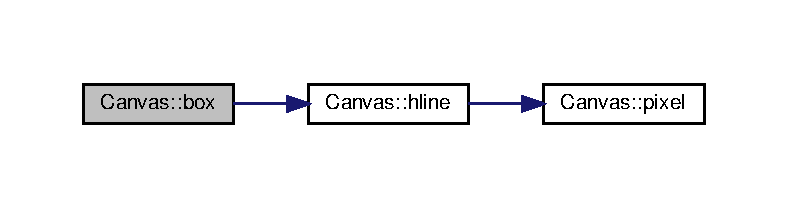
\includegraphics[width=350pt]{classCanvas_a6e1c6baa6fb92cd3de1726b67b51aa38_cgraph}
\end{center}
\end{figure}
Here is the caller graph for this function\+:\nopagebreak
\begin{figure}[H]
\begin{center}
\leavevmode
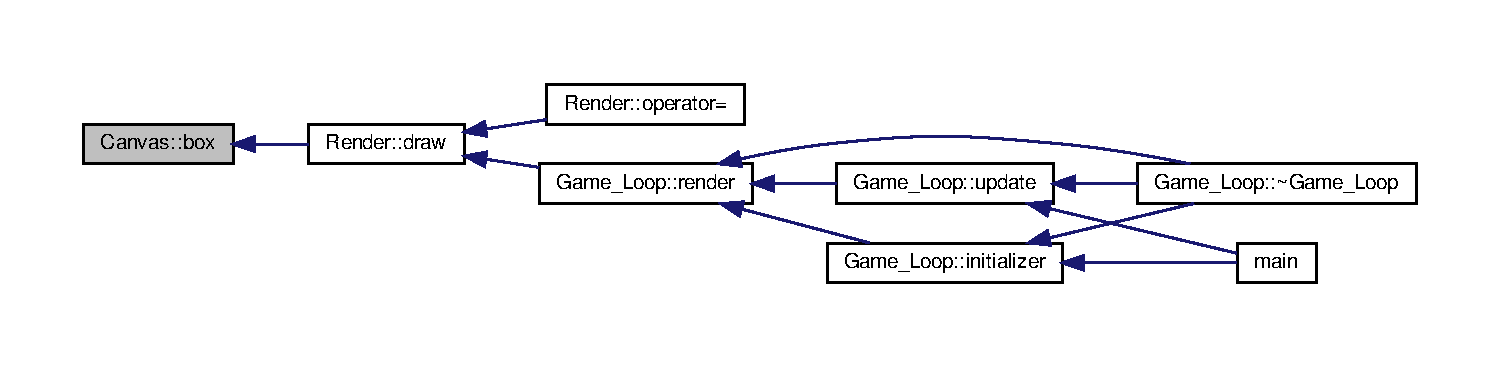
\includegraphics[width=350pt]{classCanvas_a6e1c6baa6fb92cd3de1726b67b51aa38_icgraph}
\end{center}
\end{figure}
\mbox{\Hypertarget{classCanvas_a0205269b201aed71f21b8f613cd66333}\label{classCanvas_a0205269b201aed71f21b8f613cd66333}} 
\index{Canvas@{Canvas}!clear@{clear}}
\index{clear@{clear}!Canvas@{Canvas}}
\subsubsection{\texorpdfstring{clear()}{clear()}}
{\footnotesize\ttfamily void Canvas\+::clear (\begin{DoxyParamCaption}\item[{\hyperlink{structColor}{Color}}]{color }\end{DoxyParamCaption})}



Printer the full \hyperlink{classCanvas}{Canvas} with a \hyperlink{structColor}{Color} param. 


\begin{DoxyParams}{Parameters}
{\em \hyperlink{structColor}{Color}} & color chosen to fill the \hyperlink{classCanvas}{Canvas}. \\
\hline
\end{DoxyParams}

\begin{DoxyCode}
12 \{
13     \textcolor{keywordflow}{for}( \textcolor{keywordtype}{int} i\{0\}; i <= ( m\_width * m\_height * 3 ); i+=3 )
14     \{
15         m\_pixels[i] = color.\hyperlink{structColor_ada1526285d388ff4b13e1af8d7e3ad44}{chanels}[0];
16         m\_pixels[i+1] = color.\hyperlink{structColor_ada1526285d388ff4b13e1af8d7e3ad44}{chanels}[1];
17         m\_pixels[i+2] = color.\hyperlink{structColor_ada1526285d388ff4b13e1af8d7e3ad44}{chanels}[2];
18     \}
19 \}
\end{DoxyCode}
Here is the caller graph for this function\+:\nopagebreak
\begin{figure}[H]
\begin{center}
\leavevmode
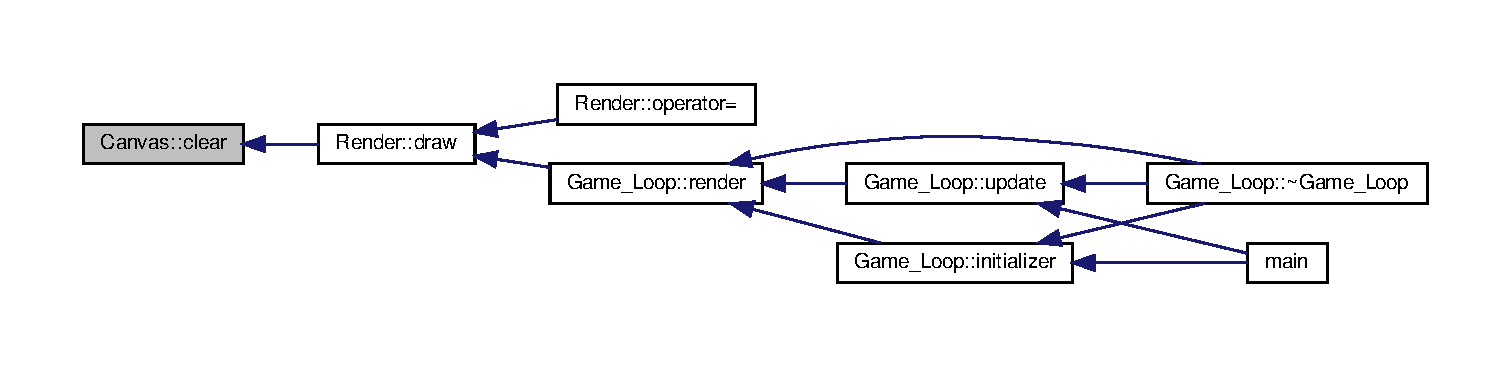
\includegraphics[width=350pt]{classCanvas_a0205269b201aed71f21b8f613cd66333_icgraph}
\end{center}
\end{figure}
\mbox{\Hypertarget{classCanvas_ab26c7ab91a0a9069895285a314bc8418}\label{classCanvas_ab26c7ab91a0a9069895285a314bc8418}} 
\index{Canvas@{Canvas}!get\+\_\+h@{get\+\_\+h}}
\index{get\+\_\+h@{get\+\_\+h}!Canvas@{Canvas}}
\subsubsection{\texorpdfstring{get\+\_\+h()}{get\_h()}}
{\footnotesize\ttfamily int Canvas\+::get\+\_\+h (\begin{DoxyParamCaption}\item[{void}]{ }\end{DoxyParamCaption}) const}



Method to get height of the \hyperlink{classCanvas}{Canvas}. 

\begin{DoxyReturn}{Returns}
int value of height 
\end{DoxyReturn}

\begin{DoxyCode}
7 \{ \textcolor{keywordflow}{return} m\_height; \}
\end{DoxyCode}
Here is the caller graph for this function\+:\nopagebreak
\begin{figure}[H]
\begin{center}
\leavevmode
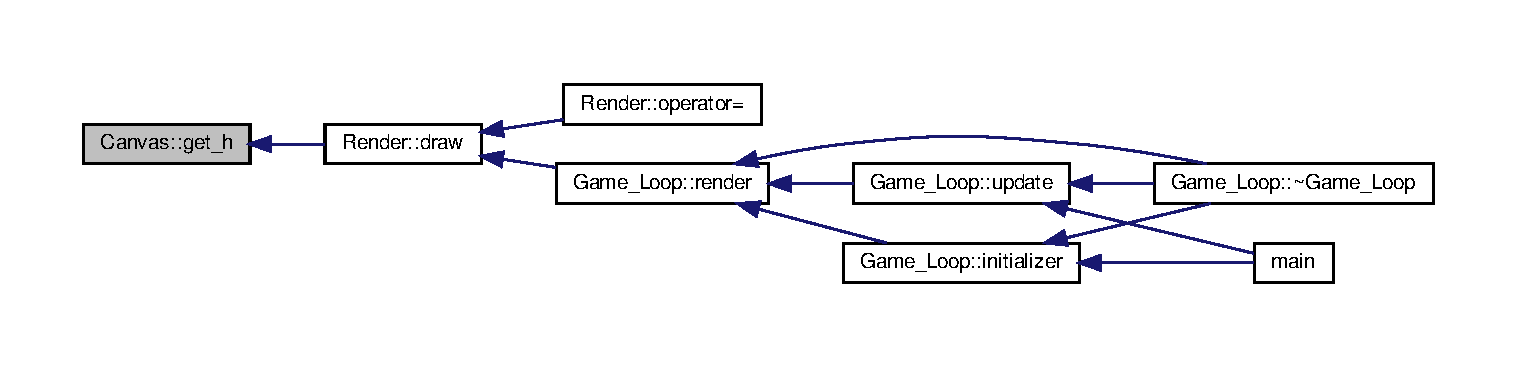
\includegraphics[width=350pt]{classCanvas_ab26c7ab91a0a9069895285a314bc8418_icgraph}
\end{center}
\end{figure}
\mbox{\Hypertarget{classCanvas_aa9f9b173d57058ea827a0134c937d0e1}\label{classCanvas_aa9f9b173d57058ea827a0134c937d0e1}} 
\index{Canvas@{Canvas}!get\+\_\+p@{get\+\_\+p}}
\index{get\+\_\+p@{get\+\_\+p}!Canvas@{Canvas}}
\subsubsection{\texorpdfstring{get\+\_\+p()}{get\_p()}}
{\footnotesize\ttfamily \hyperlink{canvas_8h_a0c8186d9b9b7880309c27230bbb5e69d}{byte} $\ast$ Canvas\+::get\+\_\+p (\begin{DoxyParamCaption}\item[{void}]{ }\end{DoxyParamCaption}) const}



Method to get the Point of the begin \hyperlink{classCanvas}{Canvas}. 

\begin{DoxyReturn}{Returns}
A Point to a byte( Unsigned char ) 
\end{DoxyReturn}

\begin{DoxyCode}
9 \{ \textcolor{keywordflow}{return} m\_pixels; \}
\end{DoxyCode}
Here is the caller graph for this function\+:\nopagebreak
\begin{figure}[H]
\begin{center}
\leavevmode
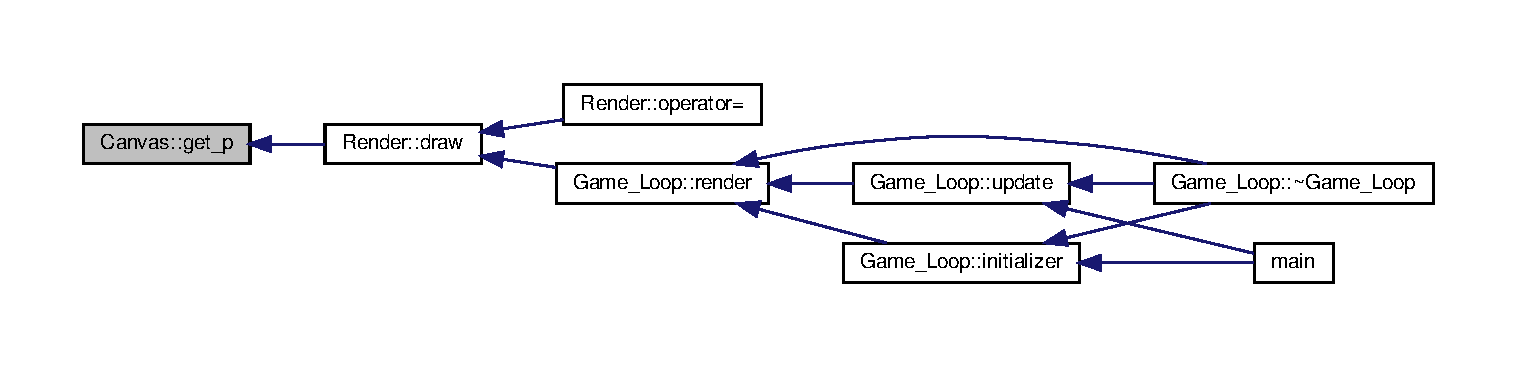
\includegraphics[width=350pt]{classCanvas_aa9f9b173d57058ea827a0134c937d0e1_icgraph}
\end{center}
\end{figure}
\mbox{\Hypertarget{classCanvas_a8478392f133ddaf1c9b7272a301c7898}\label{classCanvas_a8478392f133ddaf1c9b7272a301c7898}} 
\index{Canvas@{Canvas}!get\+\_\+w@{get\+\_\+w}}
\index{get\+\_\+w@{get\+\_\+w}!Canvas@{Canvas}}
\subsubsection{\texorpdfstring{get\+\_\+w()}{get\_w()}}
{\footnotesize\ttfamily int Canvas\+::get\+\_\+w (\begin{DoxyParamCaption}\item[{void}]{ }\end{DoxyParamCaption}) const}



Method to get width of the \hyperlink{classCanvas}{Canvas}. 

\begin{DoxyReturn}{Returns}
int value of width 
\end{DoxyReturn}

\begin{DoxyCode}
5 \{ \textcolor{keywordflow}{return} m\_width; \}
\end{DoxyCode}
Here is the caller graph for this function\+:\nopagebreak
\begin{figure}[H]
\begin{center}
\leavevmode
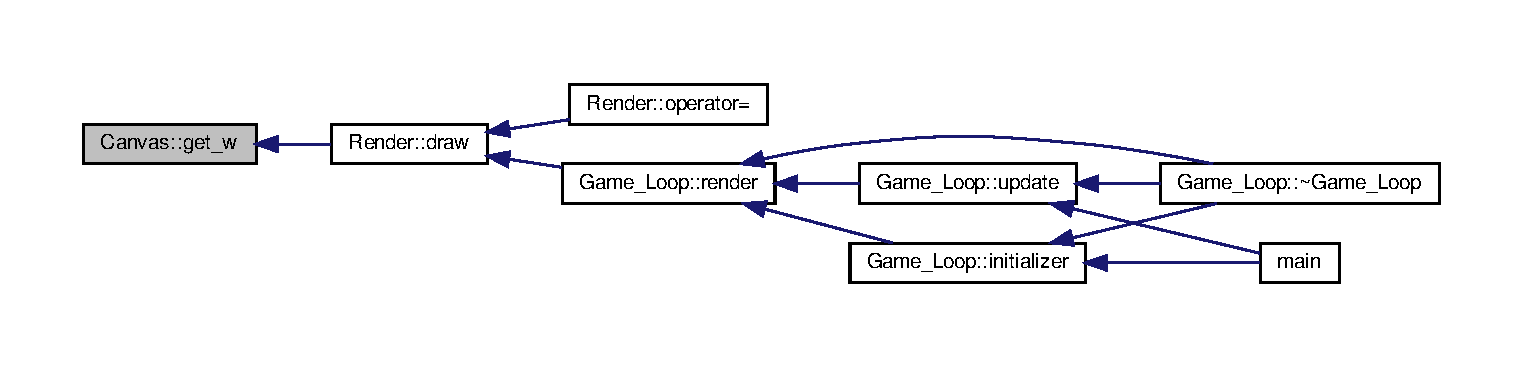
\includegraphics[width=350pt]{classCanvas_a8478392f133ddaf1c9b7272a301c7898_icgraph}
\end{center}
\end{figure}
\mbox{\Hypertarget{classCanvas_a3095d5ff2670c5dc9939454198865ceb}\label{classCanvas_a3095d5ff2670c5dc9939454198865ceb}} 
\index{Canvas@{Canvas}!hline@{hline}}
\index{hline@{hline}!Canvas@{Canvas}}
\subsubsection{\texorpdfstring{hline()}{hline()}}
{\footnotesize\ttfamily void Canvas\+::hline (\begin{DoxyParamCaption}\item[{const int \&}]{x,  }\item[{const int \&}]{y,  }\item[{const int \&}]{w,  }\item[{\hyperlink{structColor}{Color}}]{color }\end{DoxyParamCaption})}



Printer a Horizontal line. 


\begin{DoxyParams}{Parameters}
{\em const} & int \& x coordinate X on \hyperlink{classCanvas}{Canvas}. \\
\hline
{\em const} & int \& y coordiante Y on \hyperlink{classCanvas}{Canvas}. \\
\hline
{\em const} & int \& w width( S\+I\+Z\+E ) of line. \\
\hline
{\em \hyperlink{structColor}{Color}} & color color chosen to fill the line \\
\hline
\end{DoxyParams}

\begin{DoxyCode}
22 \{
23     \textcolor{keywordflow}{for}( \textcolor{keywordtype}{int} i\{0\}; i < w; i++ )
24     \{
25         \hyperlink{classCanvas_aa189a705135fb14f427747084763143a}{pixel}( x+i , y,color );
26     \}
27 \}
\end{DoxyCode}
Here is the call graph for this function\+:\nopagebreak
\begin{figure}[H]
\begin{center}
\leavevmode
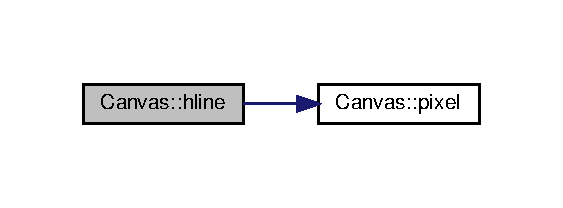
\includegraphics[width=270pt]{classCanvas_a3095d5ff2670c5dc9939454198865ceb_cgraph}
\end{center}
\end{figure}
Here is the caller graph for this function\+:\nopagebreak
\begin{figure}[H]
\begin{center}
\leavevmode
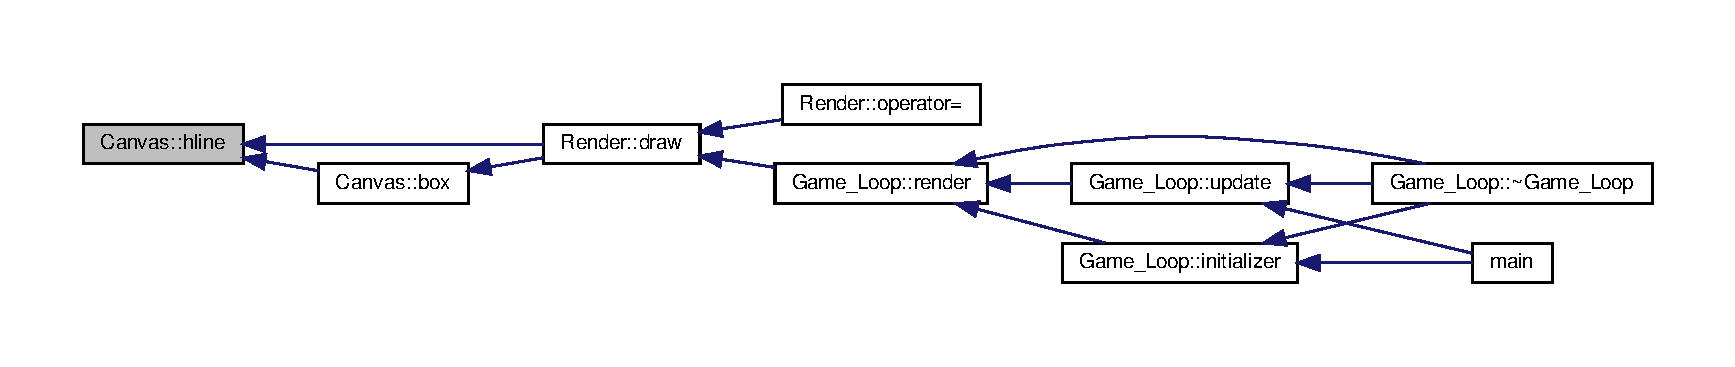
\includegraphics[width=350pt]{classCanvas_a3095d5ff2670c5dc9939454198865ceb_icgraph}
\end{center}
\end{figure}
\mbox{\Hypertarget{classCanvas_a2b44607cedf966c39c1e7c2b4abcb880}\label{classCanvas_a2b44607cedf966c39c1e7c2b4abcb880}} 
\index{Canvas@{Canvas}!operator=@{operator=}}
\index{operator=@{operator=}!Canvas@{Canvas}}
\subsubsection{\texorpdfstring{operator=()}{operator=()}}
{\footnotesize\ttfamily \hyperlink{classCanvas}{Canvas}\& Canvas\+::operator= (\begin{DoxyParamCaption}\item[{const \hyperlink{classCanvas}{Canvas} \&}]{c }\end{DoxyParamCaption})\hspace{0.3cm}{\ttfamily [inline]}}



! Assignment operator. 


\begin{DoxyCode}
61         \{
62             this->m\_width = c.m\_width;
63             this->m\_height = c.m\_height;
64             \hyperlink{canvas_8h_a0c8186d9b9b7880309c27230bbb5e69d}{byte} *ptr\{ \textcolor{keyword}{new} \hyperlink{canvas_8h_a0c8186d9b9b7880309c27230bbb5e69d}{byte}[m\_width * m\_height * 3]\};
65             *ptr = *c.m\_pixels;
66 
67             \textcolor{keywordflow}{return} *\textcolor{keyword}{this};
68         \}
\end{DoxyCode}
\mbox{\Hypertarget{classCanvas_aa189a705135fb14f427747084763143a}\label{classCanvas_aa189a705135fb14f427747084763143a}} 
\index{Canvas@{Canvas}!pixel@{pixel}}
\index{pixel@{pixel}!Canvas@{Canvas}}
\subsubsection{\texorpdfstring{pixel()}{pixel()}}
{\footnotesize\ttfamily void Canvas\+::pixel (\begin{DoxyParamCaption}\item[{const int \&}]{x,  }\item[{const int \&}]{y,  }\item[{\hyperlink{structColor}{Color}}]{color }\end{DoxyParamCaption})}



Printer a single pixel on canvs. 


\begin{DoxyParams}{Parameters}
{\em const} & int \& x coordinate X on box. \\
\hline
{\em const} & int \& y coordiante Y on box. \\
\hline
{\em \hyperlink{structColor}{Color}} & color color chosen to fill the box \\
\hline
\end{DoxyParams}

\begin{DoxyCode}
45 \{
46     m\_pixels[ ( y*m\_width*3 ) + x*3 ] = color.\hyperlink{structColor_ada1526285d388ff4b13e1af8d7e3ad44}{chanels}[0];
47     m\_pixels[ ( y*m\_width*3 ) + x*3 +1] = color.\hyperlink{structColor_ada1526285d388ff4b13e1af8d7e3ad44}{chanels}[1];
48     m\_pixels[ ( y*m\_width*3 ) + x*3 +2] = color.\hyperlink{structColor_ada1526285d388ff4b13e1af8d7e3ad44}{chanels}[2];   
49 \}
\end{DoxyCode}
Here is the caller graph for this function\+:\nopagebreak
\begin{figure}[H]
\begin{center}
\leavevmode
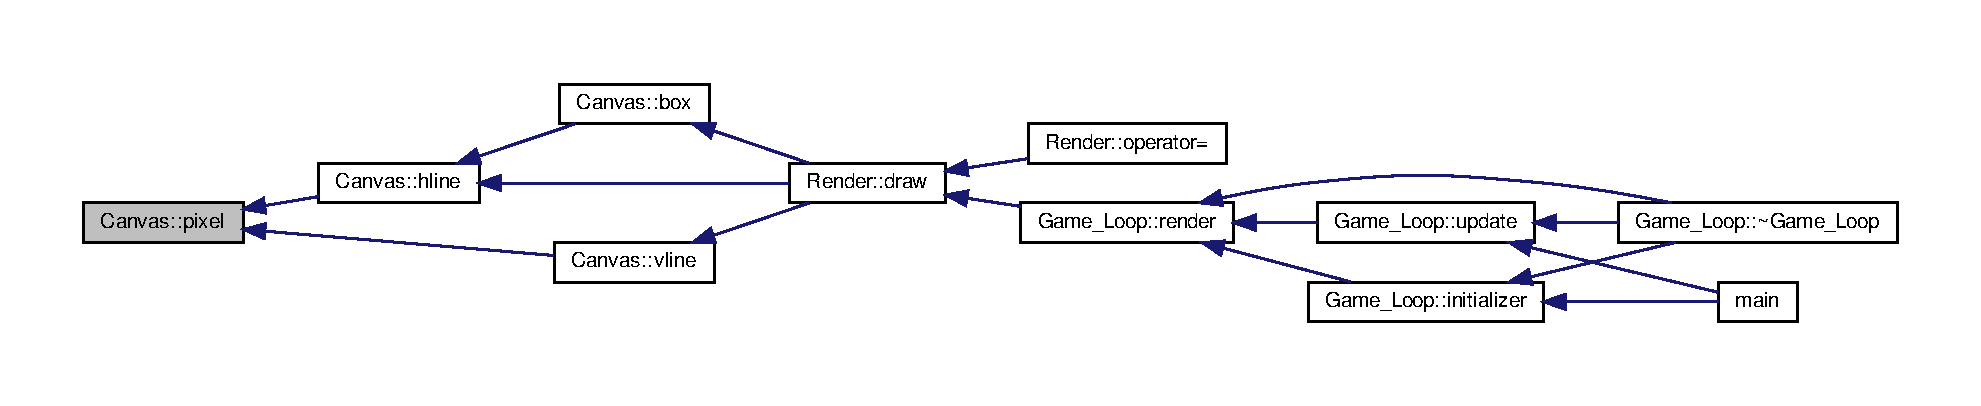
\includegraphics[width=350pt]{classCanvas_aa189a705135fb14f427747084763143a_icgraph}
\end{center}
\end{figure}
\mbox{\Hypertarget{classCanvas_af81ae19142bc132665e053ce5de15211}\label{classCanvas_af81ae19142bc132665e053ce5de15211}} 
\index{Canvas@{Canvas}!vline@{vline}}
\index{vline@{vline}!Canvas@{Canvas}}
\subsubsection{\texorpdfstring{vline()}{vline()}}
{\footnotesize\ttfamily void Canvas\+::vline (\begin{DoxyParamCaption}\item[{const int \&}]{x,  }\item[{const int \&}]{y,  }\item[{const int \&}]{h,  }\item[{\hyperlink{structColor}{Color}}]{color }\end{DoxyParamCaption})}



Printer a Vertical line. 


\begin{DoxyParams}{Parameters}
{\em const} & int \& x coordinate X on \hyperlink{classCanvas}{Canvas}. \\
\hline
{\em const} & int \& y coordiante Y on \hyperlink{classCanvas}{Canvas}. \\
\hline
{\em const} & int \& h height( S\+I\+Z\+E ) of line. \\
\hline
{\em \hyperlink{structColor}{Color}} & color color chosen to fill the line \\
\hline
\end{DoxyParams}

\begin{DoxyCode}
30 \{
31     \textcolor{keywordflow}{for}( \textcolor{keywordtype}{int} i\{0\}; i < h; i++ )
32     \{
33         \hyperlink{classCanvas_aa189a705135fb14f427747084763143a}{pixel}( x, y+i , color );
34     \}
35 \}
\end{DoxyCode}
Here is the call graph for this function\+:\nopagebreak
\begin{figure}[H]
\begin{center}
\leavevmode
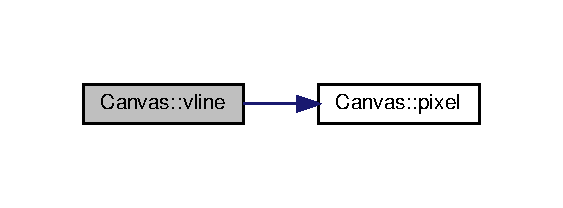
\includegraphics[width=270pt]{classCanvas_af81ae19142bc132665e053ce5de15211_cgraph}
\end{center}
\end{figure}
Here is the caller graph for this function\+:\nopagebreak
\begin{figure}[H]
\begin{center}
\leavevmode
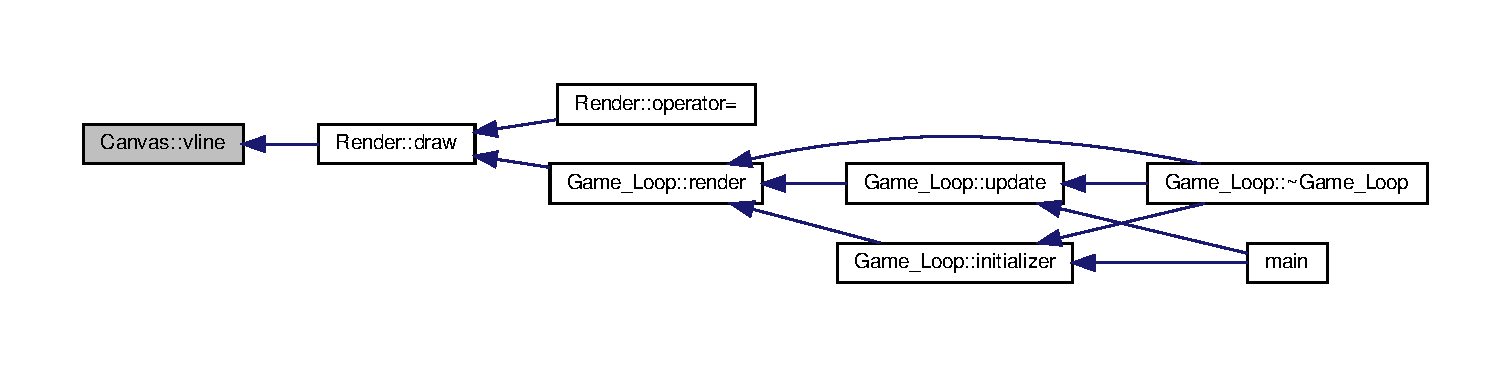
\includegraphics[width=350pt]{classCanvas_af81ae19142bc132665e053ce5de15211_icgraph}
\end{center}
\end{figure}


The documentation for this class was generated from the following files\+:\begin{DoxyCompactItemize}
\item 
/home/bergony/lp\+\_\+magos/include/\hyperlink{canvas_8h}{canvas.\+h}\item 
/home/bergony/lp\+\_\+magos/src/\hyperlink{canvas_8cpp}{canvas.\+cpp}\end{DoxyCompactItemize}

\hypertarget{structColor}{}\section{Color Struct Reference}
\label{structColor}\index{Color@{Color}}


{\bfseries Struct} \hyperlink{structColor}{Color} {\itshape  \hyperlink{structColor}{Color} of to printer.}  




{\ttfamily \#include $<$canvas.\+h$>$}

\subsection*{Public Member Functions}
\begin{DoxyCompactItemize}
\item 
\hyperlink{structColor_aa67eb05b5209dd20c279245f3043583b}{Color} (\hyperlink{canvas_8h_a0c8186d9b9b7880309c27230bbb5e69d}{byte} red=0, \hyperlink{canvas_8h_a0c8186d9b9b7880309c27230bbb5e69d}{byte} green=0, \hyperlink{canvas_8h_a0c8186d9b9b7880309c27230bbb5e69d}{byte} blue=0)
\begin{DoxyCompactList}\small\item\em ! Constructor \hyperlink{structColor}{Color} with black space. \end{DoxyCompactList}\end{DoxyCompactItemize}
\subsection*{Public Attributes}
\begin{DoxyCompactItemize}
\item 
\hyperlink{canvas_8h_a0c8186d9b9b7880309c27230bbb5e69d}{byte} \hyperlink{structColor_ada1526285d388ff4b13e1af8d7e3ad44}{chanels} \mbox{[}3\mbox{]}
\begin{DoxyCompactList}\small\item\em Byte to save Colorss. \end{DoxyCompactList}\end{DoxyCompactItemize}


\subsection{Detailed Description}
{\bfseries Struct} \hyperlink{structColor}{Color} {\itshape  \hyperlink{structColor}{Color} of to printer.} 

\subsection{Constructor \& Destructor Documentation}
\mbox{\Hypertarget{structColor_aa67eb05b5209dd20c279245f3043583b}\label{structColor_aa67eb05b5209dd20c279245f3043583b}} 
\index{Color@{Color}!Color@{Color}}
\index{Color@{Color}!Color@{Color}}
\subsubsection{\texorpdfstring{Color()}{Color()}}
{\footnotesize\ttfamily Color\+::\+Color (\begin{DoxyParamCaption}\item[{\hyperlink{canvas_8h_a0c8186d9b9b7880309c27230bbb5e69d}{byte}}]{red = {\ttfamily 0},  }\item[{\hyperlink{canvas_8h_a0c8186d9b9b7880309c27230bbb5e69d}{byte}}]{green = {\ttfamily 0},  }\item[{\hyperlink{canvas_8h_a0c8186d9b9b7880309c27230bbb5e69d}{byte}}]{blue = {\ttfamily 0} }\end{DoxyParamCaption})\hspace{0.3cm}{\ttfamily [inline]}}



! Constructor \hyperlink{structColor}{Color} with black space. 


\begin{DoxyCode}
15                                                           : \hyperlink{structColor_ada1526285d388ff4b13e1af8d7e3ad44}{chanels}
16     \{ red,          green,           blue \}
17     \{ \textcolor{comment}{/*EMPTY*/} \}
\end{DoxyCode}


\subsection{Member Data Documentation}
\mbox{\Hypertarget{structColor_ada1526285d388ff4b13e1af8d7e3ad44}\label{structColor_ada1526285d388ff4b13e1af8d7e3ad44}} 
\index{Color@{Color}!chanels@{chanels}}
\index{chanels@{chanels}!Color@{Color}}
\subsubsection{\texorpdfstring{chanels}{chanels}}
{\footnotesize\ttfamily \hyperlink{canvas_8h_a0c8186d9b9b7880309c27230bbb5e69d}{byte} Color\+::chanels\mbox{[}3\mbox{]}}



Byte to save Colorss. 



The documentation for this struct was generated from the following file\+:\begin{DoxyCompactItemize}
\item 
/home/bergony/lp\+\_\+magos/include/\hyperlink{canvas_8h}{canvas.\+h}\end{DoxyCompactItemize}

\hypertarget{classGame__Loop}{}\section{Game\+\_\+\+Loop Class Reference}
\label{classGame__Loop}\index{Game\+\_\+\+Loop@{Game\+\_\+\+Loop}}


{\bfseries Class} Game\+\_\+loop {\itshape Class to control output. input and end of game.}  




{\ttfamily \#include $<$game\+\_\+loop.\+h$>$}

\subsection*{Public Member Functions}
\begin{DoxyCompactItemize}
\item 
\hyperlink{classGame__Loop_a3aaa9f78b2e3bd3711a0552e161d94e4}{Game\+\_\+\+Loop} (int r=1, int c=1, int w=800, int h=600)
\begin{DoxyCompactList}\small\item\em ! Constructor \hyperlink{classCanvas}{Canvas} \end{DoxyCompactList}\item 
\hyperlink{classGame__Loop_a874fb59c1f7dc60273fc5541046838b9}{$\sim$\+Game\+\_\+\+Loop} ()
\begin{DoxyCompactList}\small\item\em ! Destructors \hyperlink{classCanvas}{Canvas} \end{DoxyCompactList}\item 
void \hyperlink{classGame__Loop_a637d18a3f2c22b5ecd4c3f1905e52b88}{initializer} (void)
\begin{DoxyCompactList}\small\item\em ! Method to check if the param are and set \hyperlink{classMaze}{Maze} m to status default. \end{DoxyCompactList}\item 
void \hyperlink{classGame__Loop_a549ad971281e15afa38a5dc204843891}{update} (void)
\begin{DoxyCompactList}\small\item\em ! Method to make one move on build or solve if is not done.) \end{DoxyCompactList}\item 
void \hyperlink{classGame__Loop_a5048bf3b3b18b529fe1e4a474282f274}{render} (void)
\begin{DoxyCompactList}\small\item\em ! Method to render the maze in a image P\+NG on folder. \end{DoxyCompactList}\item 
bool \hyperlink{classGame__Loop_a197233063165098c509b47d9b1da3a36}{done} (void)
\begin{DoxyCompactList}\small\item\em ! Method to check if the maze is build, solve or did some error. \end{DoxyCompactList}\end{DoxyCompactItemize}


\subsection{Detailed Description}
{\bfseries Class} Game\+\_\+loop {\itshape Class to control output. input and end of game.} 

\subsection{Constructor \& Destructor Documentation}
\mbox{\Hypertarget{classGame__Loop_a3aaa9f78b2e3bd3711a0552e161d94e4}\label{classGame__Loop_a3aaa9f78b2e3bd3711a0552e161d94e4}} 
\index{Game\+\_\+\+Loop@{Game\+\_\+\+Loop}!Game\+\_\+\+Loop@{Game\+\_\+\+Loop}}
\index{Game\+\_\+\+Loop@{Game\+\_\+\+Loop}!Game\+\_\+\+Loop@{Game\+\_\+\+Loop}}
\subsubsection{\texorpdfstring{Game\+\_\+\+Loop()}{Game\_Loop()}}
{\footnotesize\ttfamily Game\+\_\+\+Loop\+::\+Game\+\_\+\+Loop (\begin{DoxyParamCaption}\item[{int}]{r = {\ttfamily 1},  }\item[{int}]{c = {\ttfamily 1},  }\item[{int}]{w = {\ttfamily 800},  }\item[{int}]{h = {\ttfamily 600} }\end{DoxyParamCaption})\hspace{0.3cm}{\ttfamily [inline]}}



! Constructor \hyperlink{classCanvas}{Canvas} 


\begin{DoxyParams}{Parameters}
{\em int} & r rows of maze \\
\hline
{\em int} & c colums of maze. \\
\hline
{\em int} & w Witdh of Image. \\
\hline
{\em int} & h Height of Image . \\
\hline
\end{DoxyParams}

\begin{DoxyCode}
48                                                                   :
49             rows\{r\}, cols\{c\}, width\{w\}, height\{h\}
50         \{
51             \hyperlink{classMaze}{Maze} m2(cols, rows);
52             m = m2;
53             \hyperlink{classBuild}{Build} b2( &m );
54             \hyperlink{classSolve}{Solve} s2( &m );
55             b = b2;
56             s = s2;
57         \}
\end{DoxyCode}
\mbox{\Hypertarget{classGame__Loop_a874fb59c1f7dc60273fc5541046838b9}\label{classGame__Loop_a874fb59c1f7dc60273fc5541046838b9}} 
\index{Game\+\_\+\+Loop@{Game\+\_\+\+Loop}!````~Game\+\_\+\+Loop@{$\sim$\+Game\+\_\+\+Loop}}
\index{````~Game\+\_\+\+Loop@{$\sim$\+Game\+\_\+\+Loop}!Game\+\_\+\+Loop@{Game\+\_\+\+Loop}}
\subsubsection{\texorpdfstring{$\sim$\+Game\+\_\+\+Loop()}{~Game\_Loop()}}
{\footnotesize\ttfamily Game\+\_\+\+Loop\+::$\sim$\+Game\+\_\+\+Loop (\begin{DoxyParamCaption}{ }\end{DoxyParamCaption})\hspace{0.3cm}{\ttfamily [inline]}}



! Destructors \hyperlink{classCanvas}{Canvas} 


\begin{DoxyCode}
60 \{\}
\end{DoxyCode}
Here is the call graph for this function\+:\nopagebreak
\begin{figure}[H]
\begin{center}
\leavevmode
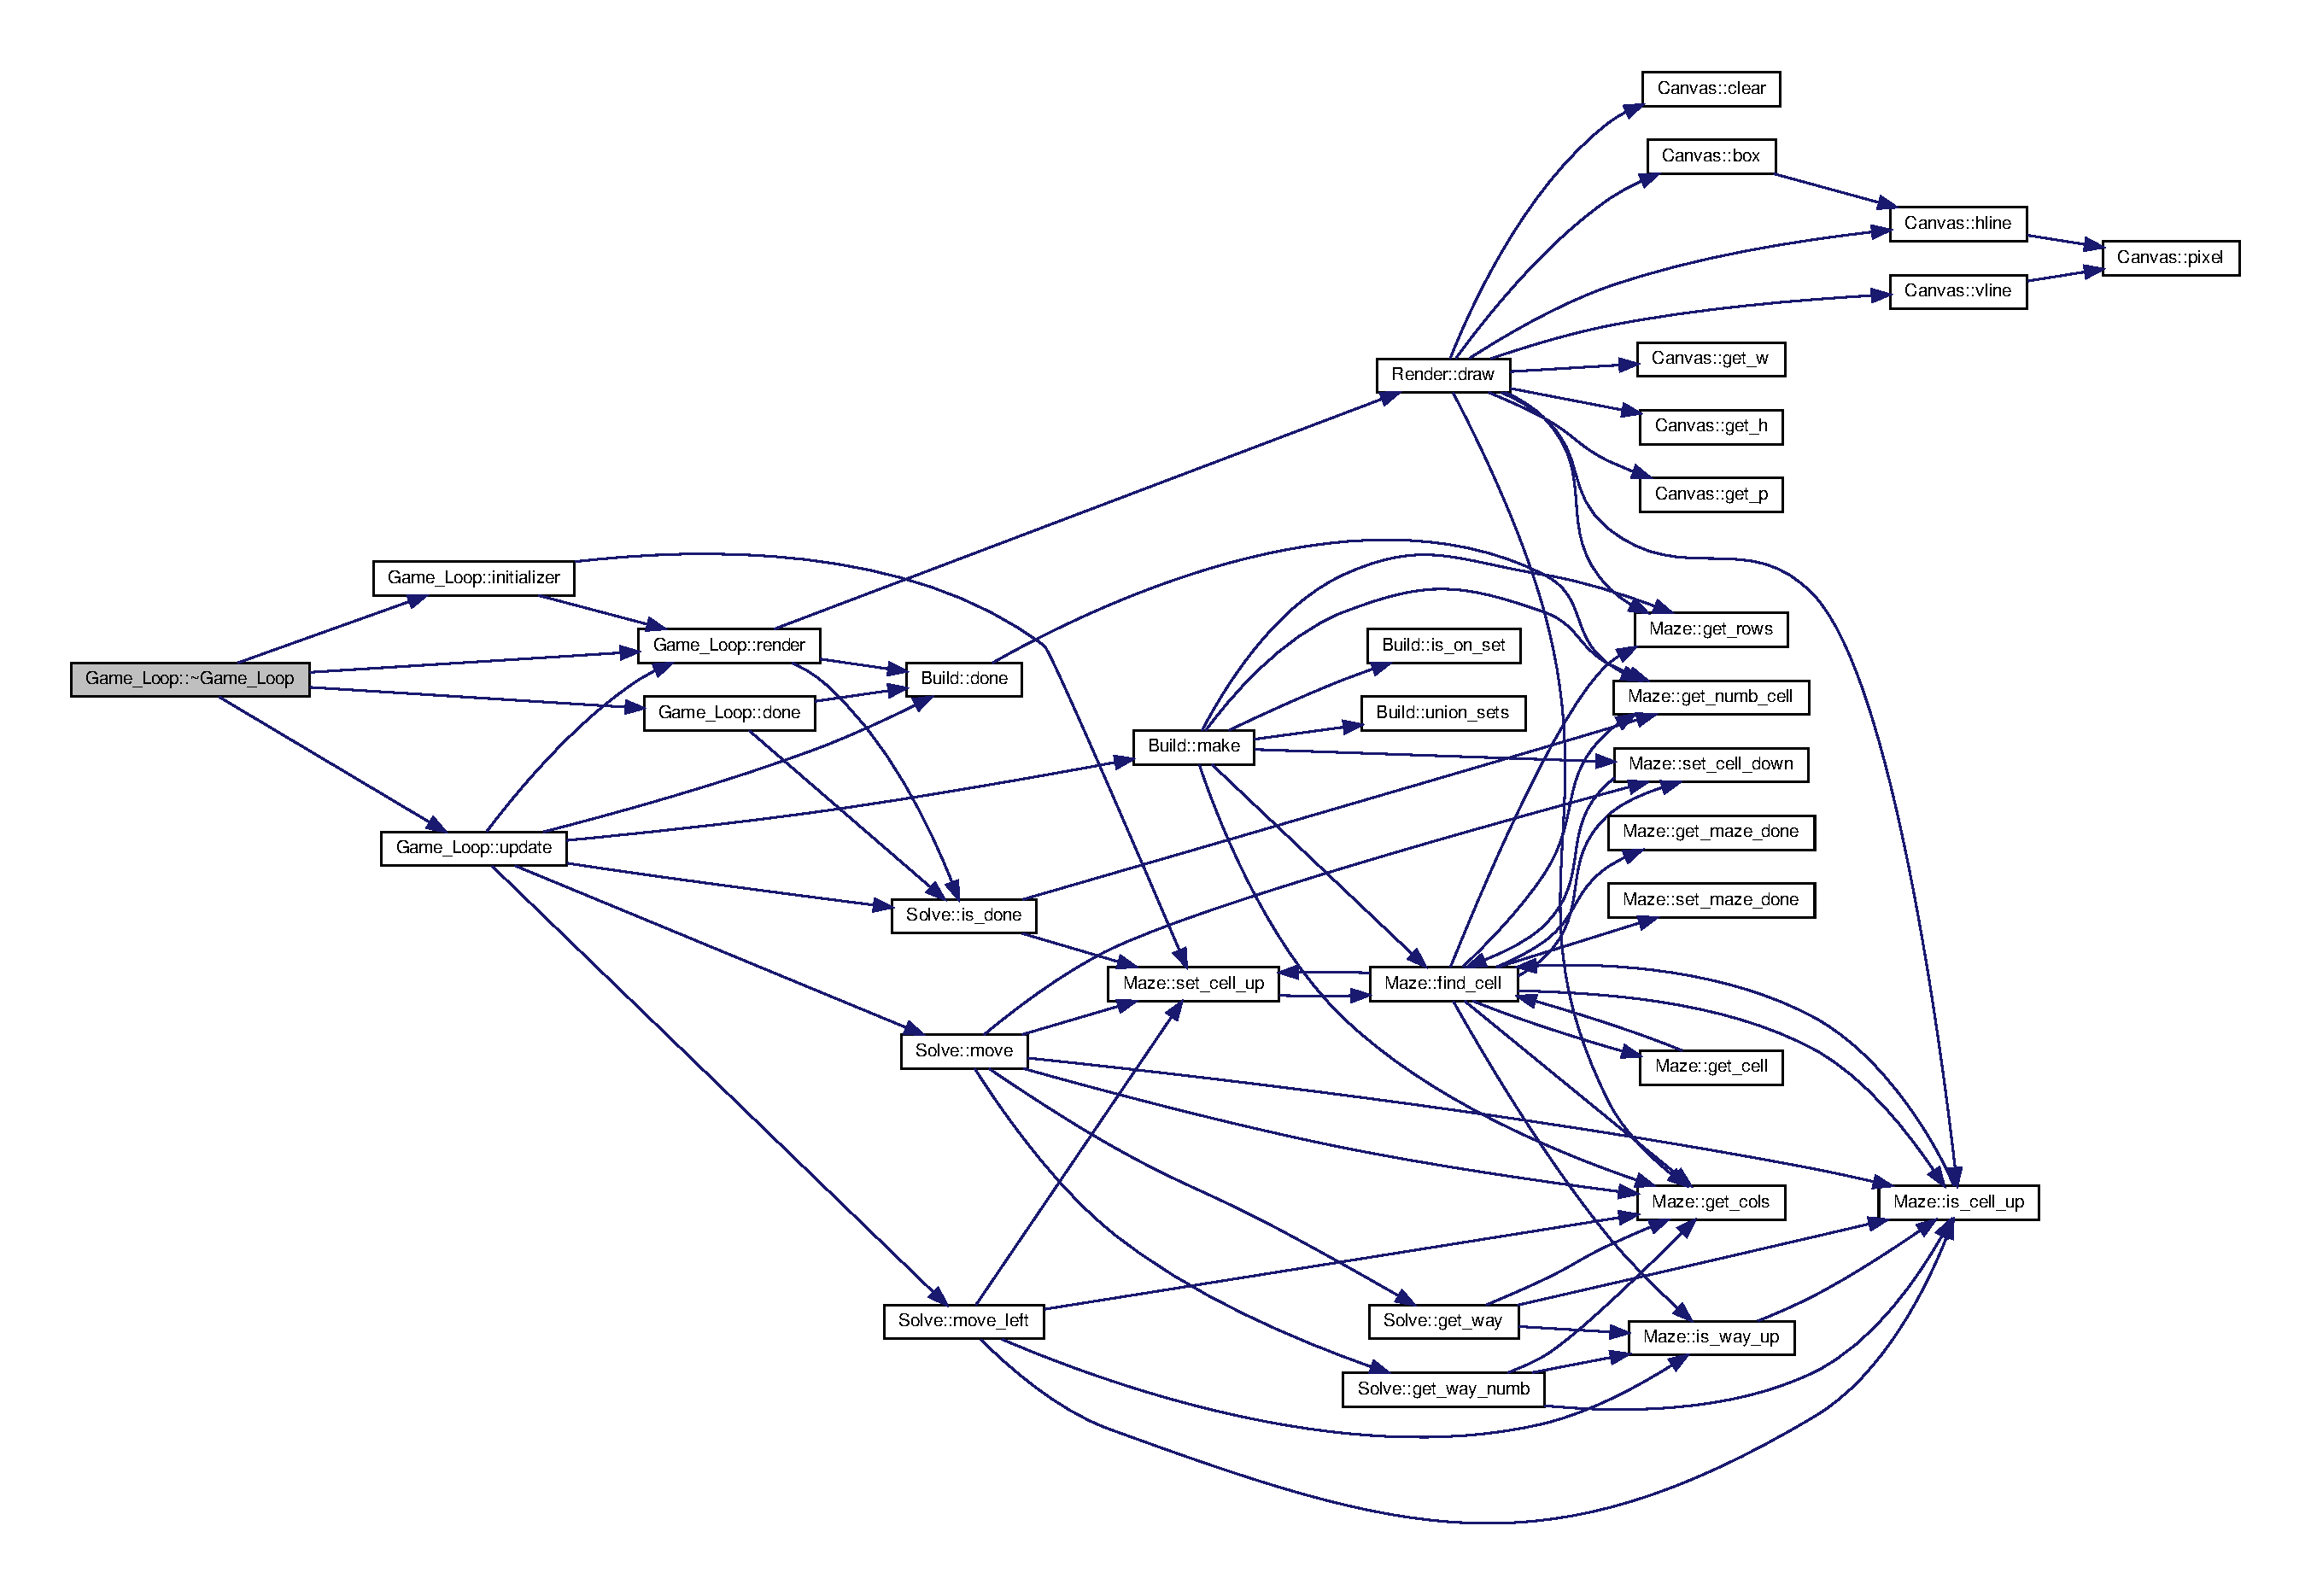
\includegraphics[width=350pt]{classGame__Loop_a874fb59c1f7dc60273fc5541046838b9_cgraph}
\end{center}
\end{figure}


\subsection{Member Function Documentation}
\mbox{\Hypertarget{classGame__Loop_a197233063165098c509b47d9b1da3a36}\label{classGame__Loop_a197233063165098c509b47d9b1da3a36}} 
\index{Game\+\_\+\+Loop@{Game\+\_\+\+Loop}!done@{done}}
\index{done@{done}!Game\+\_\+\+Loop@{Game\+\_\+\+Loop}}
\subsubsection{\texorpdfstring{done()}{done()}}
{\footnotesize\ttfamily bool Game\+\_\+\+Loop\+::done (\begin{DoxyParamCaption}\item[{void}]{ }\end{DoxyParamCaption})}



! Method to check if the maze is build, solve or did some error. 

\begin{DoxyReturn}{Returns}
True if is \hyperlink{classMaze}{Maze} Is \hyperlink{classBuild}{Build} and \hyperlink{classSolve}{Solve} or Happends any error Otherwise False. 
\end{DoxyReturn}

\begin{DoxyCode}
123 \{
124 
125     \textcolor{keywordflow}{if}( b.\hyperlink{classBuild_a72373ff38b0676c8f2c9f171c15333c4}{done}() && s.\hyperlink{classSolve_a868db181d288fdb10e5592b62e669c3b}{is\_done}() )
126     \{
127         \textcolor{keywordflow}{return} \textcolor{keyword}{true};
128     \}
129 
130     \textcolor{keywordflow}{if}(break\_loop == \textcolor{keyword}{true})
131     \{
132         std::cout << \textcolor{stringliteral}{"wrong argument numbers\(\backslash\)n"};
133         std::cout << \textcolor{stringliteral}{"One of argument are lower then configuration\(\backslash\)n"};
134         std::cout << \textcolor{stringliteral}{"lower configuration (2x3) or (3x2) and (100x100)\(\backslash\)n"};
135         \textcolor{keywordflow}{return} \textcolor{keyword}{true};
136     \}
137 
138     \textcolor{keywordflow}{return} \textcolor{keyword}{false};
139 
140 \}
\end{DoxyCode}
Here is the call graph for this function\+:\nopagebreak
\begin{figure}[H]
\begin{center}
\leavevmode
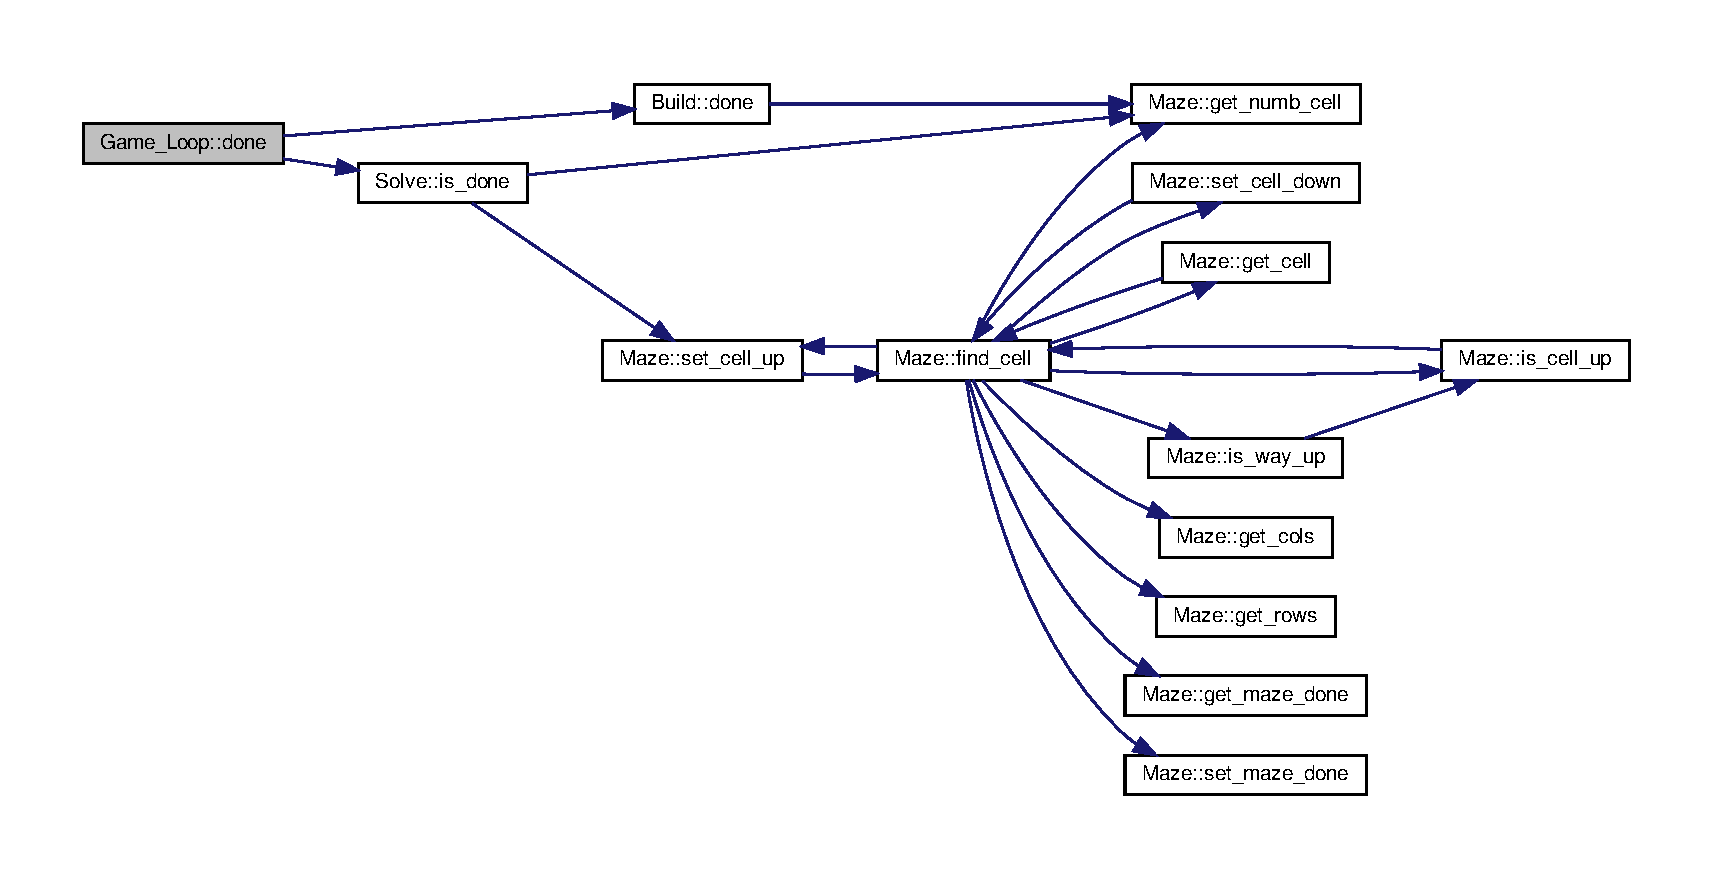
\includegraphics[width=350pt]{classGame__Loop_a197233063165098c509b47d9b1da3a36_cgraph}
\end{center}
\end{figure}
Here is the caller graph for this function\+:\nopagebreak
\begin{figure}[H]
\begin{center}
\leavevmode
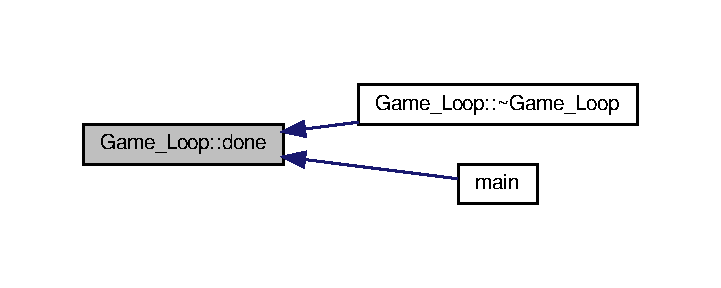
\includegraphics[width=346pt]{classGame__Loop_a197233063165098c509b47d9b1da3a36_icgraph}
\end{center}
\end{figure}
\mbox{\Hypertarget{classGame__Loop_a637d18a3f2c22b5ecd4c3f1905e52b88}\label{classGame__Loop_a637d18a3f2c22b5ecd4c3f1905e52b88}} 
\index{Game\+\_\+\+Loop@{Game\+\_\+\+Loop}!initializer@{initializer}}
\index{initializer@{initializer}!Game\+\_\+\+Loop@{Game\+\_\+\+Loop}}
\subsubsection{\texorpdfstring{initializer()}{initializer()}}
{\footnotesize\ttfamily void Game\+\_\+\+Loop\+::initializer (\begin{DoxyParamCaption}\item[{void}]{ }\end{DoxyParamCaption})}



! Method to check if the param are and set \hyperlink{classMaze}{Maze} m to status default. 


\begin{DoxyCode}
5 \{
6     \textcolor{comment}{// Set back\_track to true use back solve.}
7     \textcolor{comment}{// set back\_track to false use hand solve.}
8     back\_track = \textcolor{keyword}{false};
9     \textcolor{keywordflow}{if}( rows * 8 > width || cols * 8 > height )
10     \{
11         std::cout << \textcolor{stringliteral}{"The Canvas Size is to short to Draw\(\backslash\)n"};
12         break\_loop = \textcolor{keyword}{true};
13     \}
14     \textcolor{keywordflow}{if}(rows < 2 || cols < 2)
15     \{
16         std::cout << \textcolor{stringliteral}{"The Rows our Coluns is under the range"};
17         break\_loop = \textcolor{keyword}{true};
18     \}
19 
20     \textcolor{keywordflow}{if}(width < 100 || height < 100)
21     \{
22 
23         std::cout << \textcolor{stringliteral}{"The width or he height is under the range"};
24         break\_loop = \textcolor{keyword}{true};
25     \}
26     \textcolor{keywordflow}{if}(rows == 2 && cols == 2 )
27     \{
28 
29         std::cout << \textcolor{stringliteral}{"The Rows and coluns are under the range"};
30         break\_loop = \textcolor{keyword}{true};
31     \}
32     m.\hyperlink{classMaze_aa7c832a91a3db8f48b31f688332f8986}{set\_cell\_up}(0,0, \hyperlink{classMaze_a07167e321eac2b67100fb82ecb98f1d1a31f57c97180bdc320a97370c71cf524a}{Maze::status\_cell::entrace});
33     \textcolor{keywordflow}{for}( \textcolor{keywordtype}{int} i\{0\}; i < rows; i++)
34     \{
35         \textcolor{keywordflow}{for}(\textcolor{keywordtype}{int} j\{0\}; j < cols; j++)
36         \{
37             m.\hyperlink{classMaze_aa7c832a91a3db8f48b31f688332f8986}{set\_cell\_up}( i,j, \hyperlink{classMaze_a07167e321eac2b67100fb82ecb98f1d1ab28354b543375bfa94dabaeda722927f}{Maze::status\_cell::top} );
38             m.\hyperlink{classMaze_aa7c832a91a3db8f48b31f688332f8986}{set\_cell\_up}( i,j, \hyperlink{classMaze_a07167e321eac2b67100fb82ecb98f1d1a74e8333ad11685ff3bdae589c8f6e34d}{Maze::status\_cell::down} );
39             m.\hyperlink{classMaze_aa7c832a91a3db8f48b31f688332f8986}{set\_cell\_up}( i,j, \hyperlink{classMaze_a07167e321eac2b67100fb82ecb98f1d1a811882fecd5c7618d7099ebbd39ea254}{Maze::status\_cell::left} );
40             m.\hyperlink{classMaze_aa7c832a91a3db8f48b31f688332f8986}{set\_cell\_up}( i,j, \hyperlink{classMaze_a07167e321eac2b67100fb82ecb98f1d1a7c4f29407893c334a6cb7a87bf045c0d}{Maze::status\_cell::right} );
41         \}
42     \}
43     m.\hyperlink{classMaze_aa7c832a91a3db8f48b31f688332f8986}{set\_cell\_up}(rows-1,cols-1, \hyperlink{classMaze_a07167e321eac2b67100fb82ecb98f1d1af24f62eeb789199b9b2e467df3b1876b}{Maze::status\_cell::exit});
44 
45     \hyperlink{classGame__Loop_a5048bf3b3b18b529fe1e4a474282f274}{render}();
46     n\_pictures++;
47     percent = 100.0/(cols*rows);
48     std::cout << \textcolor{stringliteral}{"\(\backslash\)nBUILDING THE MAZE \(\backslash\)n"};
49     std::cout << std::setprecision(4) << percent << \textcolor{stringliteral}{"%\(\backslash\)n"};
50 \}
\end{DoxyCode}
Here is the call graph for this function\+:\nopagebreak
\begin{figure}[H]
\begin{center}
\leavevmode
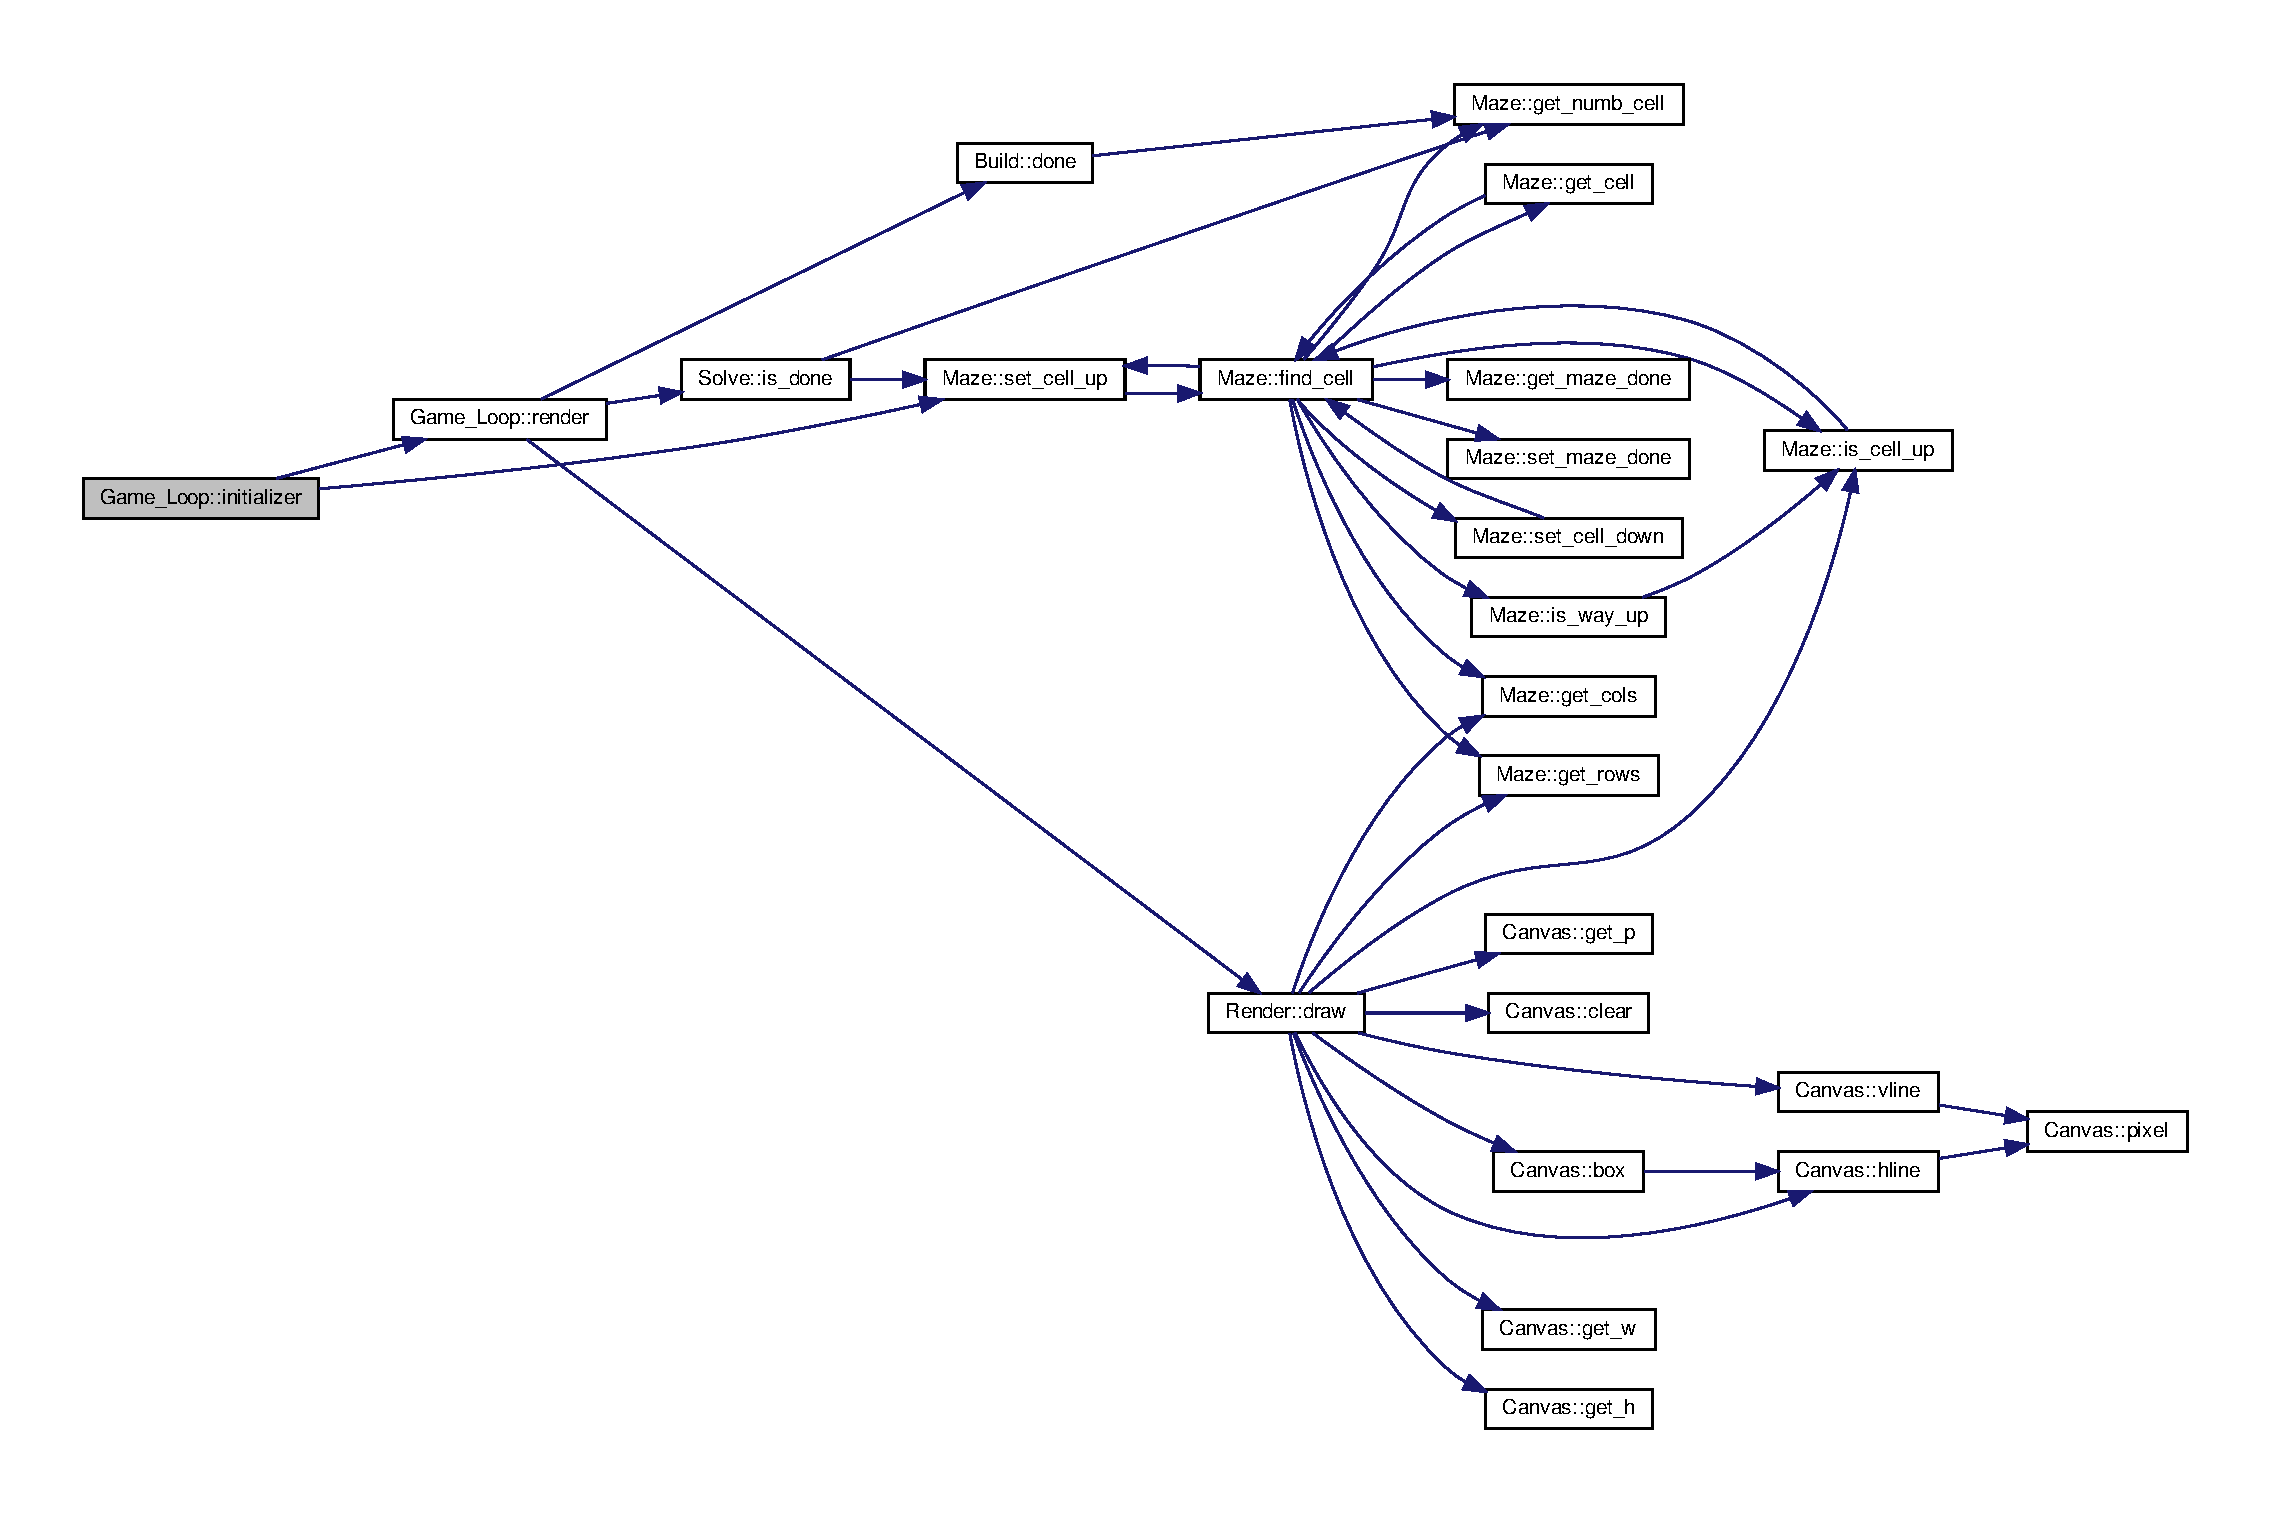
\includegraphics[width=350pt]{classGame__Loop_a637d18a3f2c22b5ecd4c3f1905e52b88_cgraph}
\end{center}
\end{figure}
Here is the caller graph for this function\+:\nopagebreak
\begin{figure}[H]
\begin{center}
\leavevmode
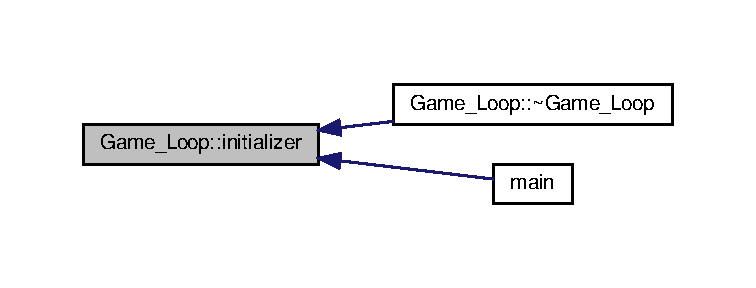
\includegraphics[width=350pt]{classGame__Loop_a637d18a3f2c22b5ecd4c3f1905e52b88_icgraph}
\end{center}
\end{figure}
\mbox{\Hypertarget{classGame__Loop_a5048bf3b3b18b529fe1e4a474282f274}\label{classGame__Loop_a5048bf3b3b18b529fe1e4a474282f274}} 
\index{Game\+\_\+\+Loop@{Game\+\_\+\+Loop}!render@{render}}
\index{render@{render}!Game\+\_\+\+Loop@{Game\+\_\+\+Loop}}
\subsubsection{\texorpdfstring{render()}{render()}}
{\footnotesize\ttfamily void Game\+\_\+\+Loop\+::render (\begin{DoxyParamCaption}\item[{void}]{ }\end{DoxyParamCaption})}



! Method to render the maze in a image P\+NG on folder. 


\begin{DoxyCode}
101 \{
102 
103     \hyperlink{classRender}{Render} rdr( &m, width , height);
104     \textcolor{keywordflow}{if}( (!b.\hyperlink{classBuild_a72373ff38b0676c8f2c9f171c15333c4}{done}() || percent != 100) && printer == \textcolor{keyword}{false}  )
105     \{   
106             output = b\_string + std::to\_string(n\_pictures);
107             rdr.draw(output);
108     \}
109 
110     \textcolor{keywordflow}{if}( b.\hyperlink{classBuild_a72373ff38b0676c8f2c9f171c15333c4}{done}() && !s.\hyperlink{classSolve_a868db181d288fdb10e5592b62e669c3b}{is\_done}())
111     \{
112         output = s\_string + std::to\_string(trys);
113         rdr.draw(output);
114     \}
115     \textcolor{keywordflow}{if}( b.\hyperlink{classBuild_a72373ff38b0676c8f2c9f171c15333c4}{done}() && s.\hyperlink{classSolve_a868db181d288fdb10e5592b62e669c3b}{is\_done}())
116     \{
117         output = s\_string + std::to\_string(trys);
118         rdr.draw(output);
119     \}
120 \}
\end{DoxyCode}
Here is the call graph for this function\+:\nopagebreak
\begin{figure}[H]
\begin{center}
\leavevmode
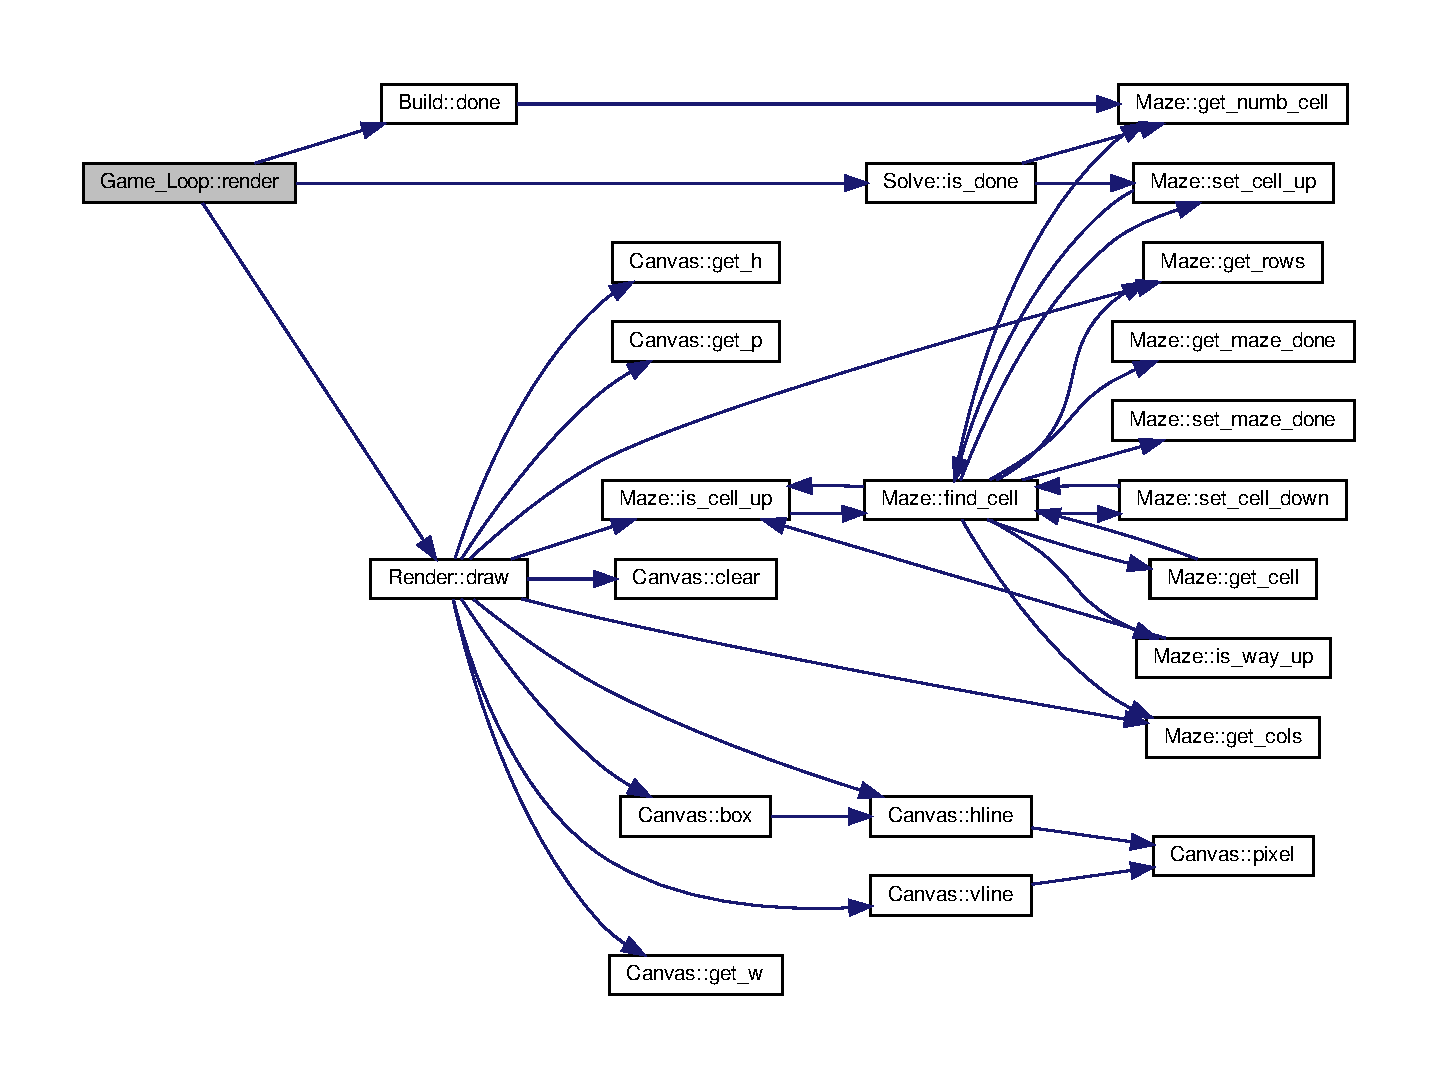
\includegraphics[width=350pt]{classGame__Loop_a5048bf3b3b18b529fe1e4a474282f274_cgraph}
\end{center}
\end{figure}
Here is the caller graph for this function\+:\nopagebreak
\begin{figure}[H]
\begin{center}
\leavevmode
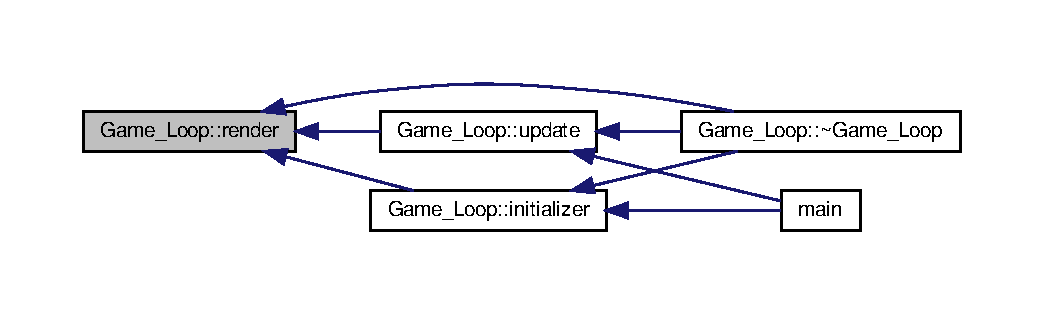
\includegraphics[width=350pt]{classGame__Loop_a5048bf3b3b18b529fe1e4a474282f274_icgraph}
\end{center}
\end{figure}
\mbox{\Hypertarget{classGame__Loop_a549ad971281e15afa38a5dc204843891}\label{classGame__Loop_a549ad971281e15afa38a5dc204843891}} 
\index{Game\+\_\+\+Loop@{Game\+\_\+\+Loop}!update@{update}}
\index{update@{update}!Game\+\_\+\+Loop@{Game\+\_\+\+Loop}}
\subsubsection{\texorpdfstring{update()}{update()}}
{\footnotesize\ttfamily void Game\+\_\+\+Loop\+::update (\begin{DoxyParamCaption}\item[{void}]{ }\end{DoxyParamCaption})}



! Method to make one move on build or solve if is not done.) 


\begin{DoxyCode}
53 \{
54     \textcolor{keywordflow}{if}(break\_loop == \textcolor{keyword}{false})
55     \{
56         \textcolor{keywordflow}{if}( !b.\hyperlink{classBuild_a72373ff38b0676c8f2c9f171c15333c4}{done}() && b.\hyperlink{classBuild_ada5111f265ee6a43832db25e8da9c3d0}{make}() )
57         \{
58             \hyperlink{classGame__Loop_a5048bf3b3b18b529fe1e4a474282f274}{render}();
59 
60             percent += 100.0/(cols*rows);
61             std::cout << std::setprecision(4) << percent << \textcolor{stringliteral}{"%\(\backslash\)n"};
62             n\_pictures++;
63         \}
64 
65         \textcolor{keywordflow}{if}( b.\hyperlink{classBuild_a72373ff38b0676c8f2c9f171c15333c4}{done}())
66         \{
67             \textcolor{keywordflow}{if}(percent <= 99 && percent > 0)
68             \{
69                 std::cout << \textcolor{stringliteral}{"100%\(\backslash\)n"};
70             \}
71             \textcolor{keywordflow}{if}(percent > 0)
72             \{
73                 std::cout << \textcolor{stringliteral}{"\(\backslash\)nSOLVING THE MAZE \(\backslash\)n"};
74                 percent = -1;
75                 printer = \textcolor{keyword}{true};
76             \}
77         \}
78 
79         \textcolor{keywordflow}{if}( b.\hyperlink{classBuild_a72373ff38b0676c8f2c9f171c15333c4}{done}() && !s.\hyperlink{classSolve_a868db181d288fdb10e5592b62e669c3b}{is\_done}())
80         \{
81             \textcolor{keywordflow}{if}(back\_track == \textcolor{keyword}{true})
82             \{
83                 s.\hyperlink{classSolve_a8902b46862c7759928495e3684054f82}{move}();
84                 std::cout << \textcolor{stringliteral}{"Solving Back "} << trys << \textcolor{stringliteral}{"Moves\(\backslash\)n"};
85                 s\_string = s\_back\_string;
86                 \hyperlink{classGame__Loop_a5048bf3b3b18b529fe1e4a474282f274}{render}();
87                 trys++;
88             \}\textcolor{keywordflow}{else}\{
89                 \textcolor{keywordflow}{if}(s.\hyperlink{classSolve_a8226032eb1d4877539f417d4fab0efde}{move\_left}())
90                 \{
91                     std::cout << \textcolor{stringliteral}{"Solving Hand "} << trys << \textcolor{stringliteral}{"Moves\(\backslash\)n"};
92                     s\_string = s\_hand\_string;
93                     \hyperlink{classGame__Loop_a5048bf3b3b18b529fe1e4a474282f274}{render}();
94                     trys++;
95                 \}
96             \}
97         \}
98     \}
99 \}
\end{DoxyCode}
Here is the call graph for this function\+:\nopagebreak
\begin{figure}[H]
\begin{center}
\leavevmode
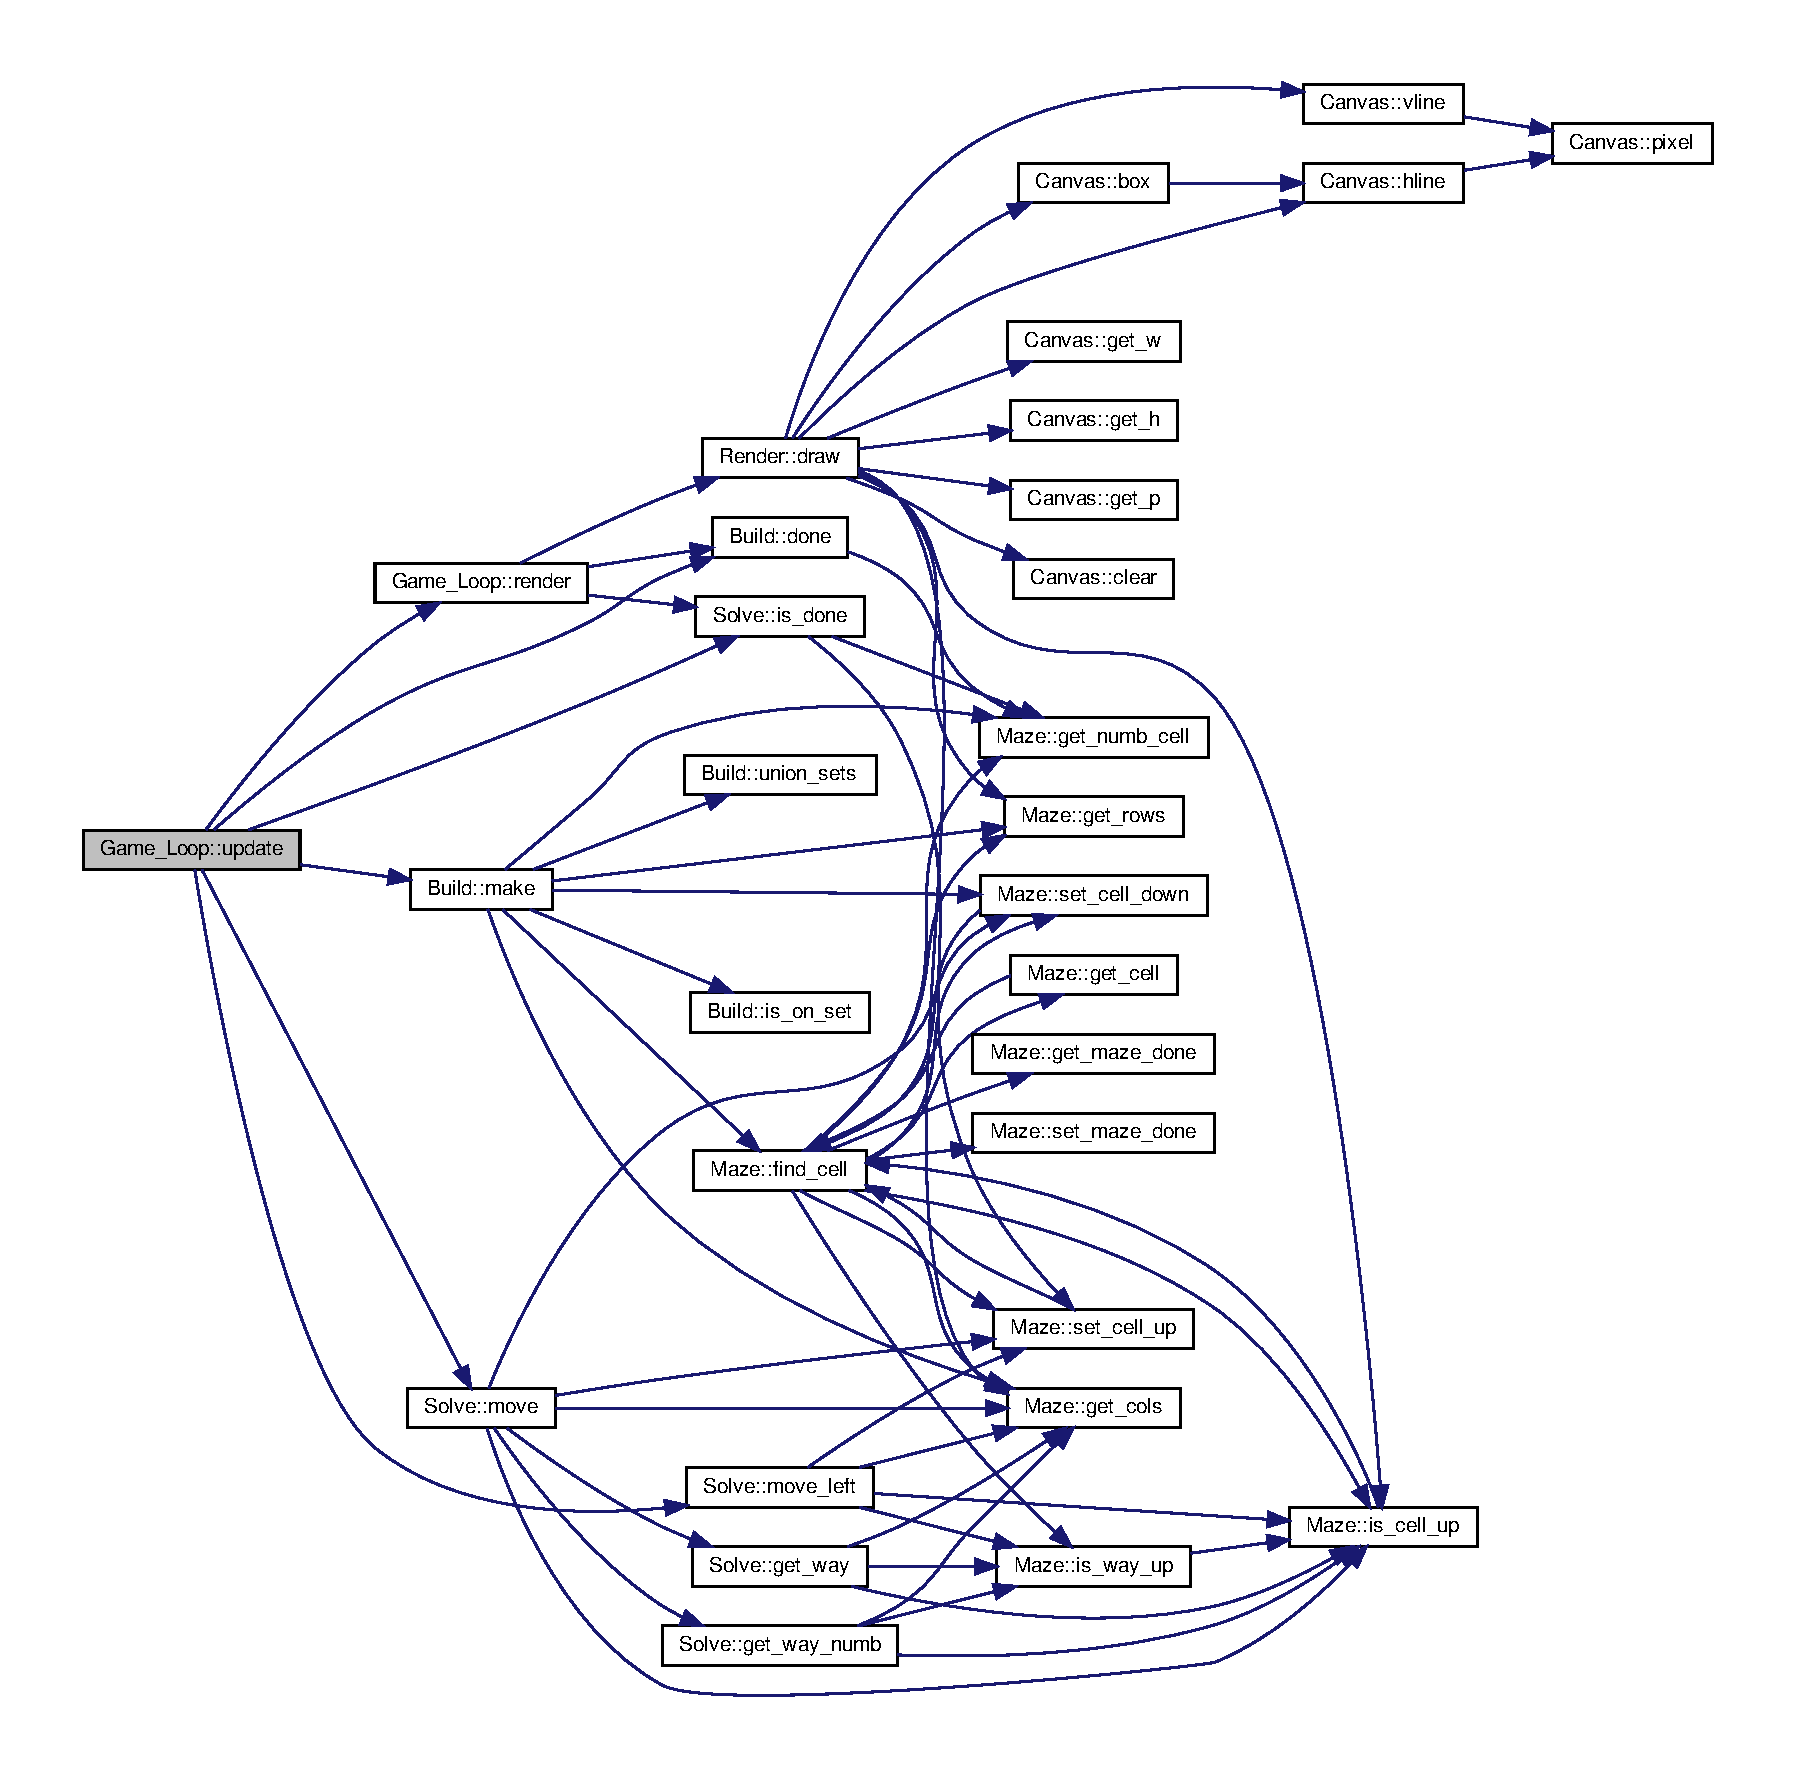
\includegraphics[width=350pt]{classGame__Loop_a549ad971281e15afa38a5dc204843891_cgraph}
\end{center}
\end{figure}
Here is the caller graph for this function\+:\nopagebreak
\begin{figure}[H]
\begin{center}
\leavevmode
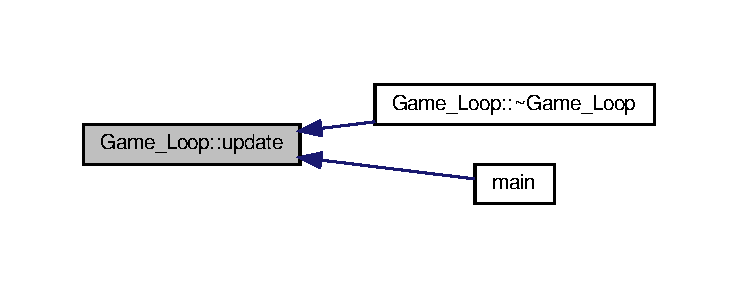
\includegraphics[width=350pt]{classGame__Loop_a549ad971281e15afa38a5dc204843891_icgraph}
\end{center}
\end{figure}


The documentation for this class was generated from the following files\+:\begin{DoxyCompactItemize}
\item 
/home/bergony/lp\+\_\+magos/include/\hyperlink{game__loop_8h}{game\+\_\+loop.\+h}\item 
/home/bergony/lp\+\_\+magos/src/\hyperlink{game__loop_8cpp}{game\+\_\+loop.\+cpp}\end{DoxyCompactItemize}

\hypertarget{classMaze}{}\section{Maze Class Reference}
\label{classMaze}\index{Maze@{Maze}}


{\bfseries Class} \hyperlink{classMaze}{Maze} {\itshape Class create a \hyperlink{classMaze}{Maze} to be \hyperlink{classBuild}{Build}, \hyperlink{classSolve}{Solve} and \hyperlink{classRender}{Render}.}  




{\ttfamily \#include $<$maze.\+h$>$}

\subsection*{Public Types}
\begin{DoxyCompactItemize}
\item 
enum \hyperlink{classMaze_a07167e321eac2b67100fb82ecb98f1d1}{status\+\_\+cell} \{ \newline
\hyperlink{classMaze_a07167e321eac2b67100fb82ecb98f1d1ab28354b543375bfa94dabaeda722927f}{status\+\_\+cell\+::top} = (bit)1, 
\hyperlink{classMaze_a07167e321eac2b67100fb82ecb98f1d1a74e8333ad11685ff3bdae589c8f6e34d}{status\+\_\+cell\+::down} = (bit)2, 
\hyperlink{classMaze_a07167e321eac2b67100fb82ecb98f1d1a811882fecd5c7618d7099ebbd39ea254}{status\+\_\+cell\+::left} = (bit)4, 
\hyperlink{classMaze_a07167e321eac2b67100fb82ecb98f1d1a7c4f29407893c334a6cb7a87bf045c0d}{status\+\_\+cell\+::right} = (bit)8, 
\newline
\hyperlink{classMaze_a07167e321eac2b67100fb82ecb98f1d1ac83b72dd001482ce10f0b106c7a0ed0e}{status\+\_\+cell\+::way} = (bit)16, 
\hyperlink{classMaze_a07167e321eac2b67100fb82ecb98f1d1a94708897ec9db8647dfe695714c98e46}{status\+\_\+cell\+::discarded} = (bit)32, 
\hyperlink{classMaze_a07167e321eac2b67100fb82ecb98f1d1a31f57c97180bdc320a97370c71cf524a}{status\+\_\+cell\+::entrace} = (bit)64, 
\hyperlink{classMaze_a07167e321eac2b67100fb82ecb98f1d1af24f62eeb789199b9b2e467df3b1876b}{status\+\_\+cell\+::exit} = (bit)128
 \}\begin{DoxyCompactList}\small\item\em {\bfseries  enum class} Status {\itshape  Type of status cell and them value.} \end{DoxyCompactList}
\end{DoxyCompactItemize}
\subsection*{Public Member Functions}
\begin{DoxyCompactItemize}
\item 
\hyperlink{classMaze_aa744020bbce986ebc4d33f30b7a2d52f}{Maze} (int c=0, int r=0)
\begin{DoxyCompactList}\small\item\em ! Constructor \hyperlink{classMaze}{Maze} \end{DoxyCompactList}\item 
\hyperlink{classMaze_a4f187353f595193318ac66133a22287e}{$\sim$\+Maze} ()
\begin{DoxyCompactList}\small\item\em ! Destructors \hyperlink{classMaze}{Maze}. \end{DoxyCompactList}\item 
\hyperlink{classMaze_ace1fa70e147e319c7ff135f1ca1bd0e3}{Maze} (const \hyperlink{classMaze}{Maze} \&clone)
\item 
\hyperlink{classMaze}{Maze} \& \hyperlink{classMaze_a41468a30ae450b06d4a07304e9cda5ed}{operator=} (const \hyperlink{classMaze}{Maze} \&m)
\begin{DoxyCompactList}\small\item\em ! Assignmentt Operator. \end{DoxyCompactList}\item 
int \hyperlink{classMaze_aa59b935dcd5f7129636cea6e40882c56}{find\+\_\+cell} (int x, int y)
\begin{DoxyCompactList}\small\item\em Method to find the cell on vector by coordinates( x, y). \end{DoxyCompactList}\item 
void \hyperlink{classMaze_aa7c832a91a3db8f48b31f688332f8986}{set\+\_\+cell\+\_\+up} (int x, int y, \hyperlink{classMaze_a07167e321eac2b67100fb82ecb98f1d1}{status\+\_\+cell} sc)
\begin{DoxyCompactList}\small\item\em Method to change bit corresponding status cell to one. \end{DoxyCompactList}\item 
void \hyperlink{classMaze_a53781b836de1a6b2c7ded74a2798b703}{set\+\_\+cell\+\_\+up} (int cell, \hyperlink{classMaze_a07167e321eac2b67100fb82ecb98f1d1}{status\+\_\+cell} sc)
\begin{DoxyCompactList}\small\item\em Method to change bit corresponding status cell to one. \end{DoxyCompactList}\item 
void \hyperlink{classMaze_ab86292a84aa56a26c4c07f4aa684d9bb}{set\+\_\+cell\+\_\+down} (int x, int y, \hyperlink{classMaze_a07167e321eac2b67100fb82ecb98f1d1}{status\+\_\+cell} sc)
\begin{DoxyCompactList}\small\item\em Method to change bit corresponding status cell to zero. \end{DoxyCompactList}\item 
void \hyperlink{classMaze_a3635b71fab2c610376ae6613e7265fdf}{set\+\_\+cell\+\_\+down} (int cell, \hyperlink{classMaze_a07167e321eac2b67100fb82ecb98f1d1}{status\+\_\+cell} sc)
\begin{DoxyCompactList}\small\item\em Method to change bit corresponding status cell to zero. \end{DoxyCompactList}\item 
\hyperlink{maze_8h_a789d352559efaa396a258805d44f4289}{bit} \hyperlink{classMaze_ae07191c6ec3cc47fce1147bc3f03a8ad}{get\+\_\+cell} (int x, int y)
\begin{DoxyCompactList}\small\item\em Method to see all status of cell. \end{DoxyCompactList}\item 
bool \hyperlink{classMaze_a2b0e69e72d6c3e1037578f057946a21e}{is\+\_\+cell\+\_\+up} (int x, int y, \hyperlink{classMaze_a07167e321eac2b67100fb82ecb98f1d1}{status\+\_\+cell} sc)
\begin{DoxyCompactList}\small\item\em Method to check if the status cell sc is up. \end{DoxyCompactList}\item 
bool \hyperlink{classMaze_ad5dd6a918e4fd4bb6392e0a0bc08b81d}{is\+\_\+cell\+\_\+up} (int cell, \hyperlink{classMaze_a07167e321eac2b67100fb82ecb98f1d1}{status\+\_\+cell} sc)
\begin{DoxyCompactList}\small\item\em Method to check if the status cell sc is up. \end{DoxyCompactList}\item 
bool \hyperlink{classMaze_a308fa695665de6217c0e7f28aab5adda}{is\+\_\+way\+\_\+up} (int cell)
\begin{DoxyCompactList}\small\item\em Method to check if the cell have be see. \end{DoxyCompactList}\item 
int \hyperlink{classMaze_a8a04cd1335e96a80358181afa164d4c9}{get\+\_\+cols} (void)
\begin{DoxyCompactList}\small\item\em Method to get numbers of colums. \end{DoxyCompactList}\item 
int \hyperlink{classMaze_ac786606a34632b2254b2d27d5f5f0f3f}{get\+\_\+rows} (void)
\begin{DoxyCompactList}\small\item\em Method to get numbers of rows. \end{DoxyCompactList}\item 
int \hyperlink{classMaze_a90f5c1c140a9991942204d4a7fec3bf8}{get\+\_\+numb\+\_\+cell} (void)
\begin{DoxyCompactList}\small\item\em Method to get numbers of cell. \end{DoxyCompactList}\item 
int \hyperlink{classMaze_a152979999dd4c75014d65bf6deb5a00c}{get\+\_\+maze\+\_\+done} (void)
\item 
void \hyperlink{classMaze_ab31ce10f6d3dfdd64d15c7b48f93ed63}{set\+\_\+maze\+\_\+done} (int x)
\end{DoxyCompactItemize}


\subsection{Detailed Description}
{\bfseries Class} \hyperlink{classMaze}{Maze} {\itshape Class create a \hyperlink{classMaze}{Maze} to be \hyperlink{classBuild}{Build}, \hyperlink{classSolve}{Solve} and \hyperlink{classRender}{Render}.} 

\subsection{Member Enumeration Documentation}
\mbox{\Hypertarget{classMaze_a07167e321eac2b67100fb82ecb98f1d1}\label{classMaze_a07167e321eac2b67100fb82ecb98f1d1}} 
\index{Maze@{Maze}!status\+\_\+cell@{status\+\_\+cell}}
\index{status\+\_\+cell@{status\+\_\+cell}!Maze@{Maze}}
\subsubsection{\texorpdfstring{status\+\_\+cell}{status\_cell}}
{\footnotesize\ttfamily enum \hyperlink{classMaze_a07167e321eac2b67100fb82ecb98f1d1}{Maze\+::status\+\_\+cell}\hspace{0.3cm}{\ttfamily [strong]}}



{\bfseries  enum class} Status {\itshape  Type of status cell and them value.} 

\begin{DoxyEnumFields}{Enumerator}
\raisebox{\heightof{T}}[0pt][0pt]{\index{top@{top}!Maze@{Maze}}\index{Maze@{Maze}!top@{top}}}\mbox{\Hypertarget{classMaze_a07167e321eac2b67100fb82ecb98f1d1ab28354b543375bfa94dabaeda722927f}\label{classMaze_a07167e321eac2b67100fb82ecb98f1d1ab28354b543375bfa94dabaeda722927f}} 
top&\\
\hline

\raisebox{\heightof{T}}[0pt][0pt]{\index{down@{down}!Maze@{Maze}}\index{Maze@{Maze}!down@{down}}}\mbox{\Hypertarget{classMaze_a07167e321eac2b67100fb82ecb98f1d1a74e8333ad11685ff3bdae589c8f6e34d}\label{classMaze_a07167e321eac2b67100fb82ecb98f1d1a74e8333ad11685ff3bdae589c8f6e34d}} 
down&\\
\hline

\raisebox{\heightof{T}}[0pt][0pt]{\index{left@{left}!Maze@{Maze}}\index{Maze@{Maze}!left@{left}}}\mbox{\Hypertarget{classMaze_a07167e321eac2b67100fb82ecb98f1d1a811882fecd5c7618d7099ebbd39ea254}\label{classMaze_a07167e321eac2b67100fb82ecb98f1d1a811882fecd5c7618d7099ebbd39ea254}} 
left&\\
\hline

\raisebox{\heightof{T}}[0pt][0pt]{\index{right@{right}!Maze@{Maze}}\index{Maze@{Maze}!right@{right}}}\mbox{\Hypertarget{classMaze_a07167e321eac2b67100fb82ecb98f1d1a7c4f29407893c334a6cb7a87bf045c0d}\label{classMaze_a07167e321eac2b67100fb82ecb98f1d1a7c4f29407893c334a6cb7a87bf045c0d}} 
right&\\
\hline

\raisebox{\heightof{T}}[0pt][0pt]{\index{way@{way}!Maze@{Maze}}\index{Maze@{Maze}!way@{way}}}\mbox{\Hypertarget{classMaze_a07167e321eac2b67100fb82ecb98f1d1ac83b72dd001482ce10f0b106c7a0ed0e}\label{classMaze_a07167e321eac2b67100fb82ecb98f1d1ac83b72dd001482ce10f0b106c7a0ed0e}} 
way&\\
\hline

\raisebox{\heightof{T}}[0pt][0pt]{\index{discarded@{discarded}!Maze@{Maze}}\index{Maze@{Maze}!discarded@{discarded}}}\mbox{\Hypertarget{classMaze_a07167e321eac2b67100fb82ecb98f1d1a94708897ec9db8647dfe695714c98e46}\label{classMaze_a07167e321eac2b67100fb82ecb98f1d1a94708897ec9db8647dfe695714c98e46}} 
discarded&\\
\hline

\raisebox{\heightof{T}}[0pt][0pt]{\index{entrace@{entrace}!Maze@{Maze}}\index{Maze@{Maze}!entrace@{entrace}}}\mbox{\Hypertarget{classMaze_a07167e321eac2b67100fb82ecb98f1d1a31f57c97180bdc320a97370c71cf524a}\label{classMaze_a07167e321eac2b67100fb82ecb98f1d1a31f57c97180bdc320a97370c71cf524a}} 
entrace&\\
\hline

\raisebox{\heightof{T}}[0pt][0pt]{\index{exit@{exit}!Maze@{Maze}}\index{Maze@{Maze}!exit@{exit}}}\mbox{\Hypertarget{classMaze_a07167e321eac2b67100fb82ecb98f1d1af24f62eeb789199b9b2e467df3b1876b}\label{classMaze_a07167e321eac2b67100fb82ecb98f1d1af24f62eeb789199b9b2e467df3b1876b}} 
exit&\\
\hline

\end{DoxyEnumFields}

\begin{DoxyCode}
26         \{
27             top = (\hyperlink{maze_8h_a789d352559efaa396a258805d44f4289}{bit})1,
28             down = (\hyperlink{maze_8h_a789d352559efaa396a258805d44f4289}{bit})2,
29             left = (\hyperlink{maze_8h_a789d352559efaa396a258805d44f4289}{bit})4,
30             right= (\hyperlink{maze_8h_a789d352559efaa396a258805d44f4289}{bit})8,
31             way = (\hyperlink{maze_8h_a789d352559efaa396a258805d44f4289}{bit})16,
32             discarded = (\hyperlink{maze_8h_a789d352559efaa396a258805d44f4289}{bit})32,
33             entrace = (\hyperlink{maze_8h_a789d352559efaa396a258805d44f4289}{bit})64,
34             exit = (\hyperlink{maze_8h_a789d352559efaa396a258805d44f4289}{bit})128
35         \};
\end{DoxyCode}


\subsection{Constructor \& Destructor Documentation}
\mbox{\Hypertarget{classMaze_aa744020bbce986ebc4d33f30b7a2d52f}\label{classMaze_aa744020bbce986ebc4d33f30b7a2d52f}} 
\index{Maze@{Maze}!Maze@{Maze}}
\index{Maze@{Maze}!Maze@{Maze}}
\subsubsection{\texorpdfstring{Maze()}{Maze()}\hspace{0.1cm}{\footnotesize\ttfamily [1/2]}}
{\footnotesize\ttfamily Maze\+::\+Maze (\begin{DoxyParamCaption}\item[{int}]{c = {\ttfamily 0},  }\item[{int}]{r = {\ttfamily 0} }\end{DoxyParamCaption})\hspace{0.3cm}{\ttfamily [inline]}}



! Constructor \hyperlink{classMaze}{Maze} 


\begin{DoxyParams}{Parameters}
{\em int} & c Numbers of colums. \\
\hline
{\em int} & r Numbers of Rows. \\
\hline
\end{DoxyParams}

\begin{DoxyCode}
43                                       :
44             m\_cols\{c\}, m\_rows\{r\}
45         \{
46             \textcolor{keywordflow}{for}(\textcolor{keywordtype}{int} i\{0\}; i < r*c; i++)
47             \{
48                 m\_cell = (\hyperlink{maze_8h_a789d352559efaa396a258805d44f4289}{bit})0;
49                 m\_cell\_list.push\_back( m\_cell );
50             \}
51         \}
\end{DoxyCode}
\mbox{\Hypertarget{classMaze_a4f187353f595193318ac66133a22287e}\label{classMaze_a4f187353f595193318ac66133a22287e}} 
\index{Maze@{Maze}!````~Maze@{$\sim$\+Maze}}
\index{````~Maze@{$\sim$\+Maze}!Maze@{Maze}}
\subsubsection{\texorpdfstring{$\sim$\+Maze()}{~Maze()}}
{\footnotesize\ttfamily Maze\+::$\sim$\+Maze (\begin{DoxyParamCaption}{ }\end{DoxyParamCaption})\hspace{0.3cm}{\ttfamily [inline]}}



! Destructors \hyperlink{classMaze}{Maze}. 


\begin{DoxyCode}
54 \{\}
\end{DoxyCode}
\mbox{\Hypertarget{classMaze_ace1fa70e147e319c7ff135f1ca1bd0e3}\label{classMaze_ace1fa70e147e319c7ff135f1ca1bd0e3}} 
\index{Maze@{Maze}!Maze@{Maze}}
\index{Maze@{Maze}!Maze@{Maze}}
\subsubsection{\texorpdfstring{Maze()}{Maze()}\hspace{0.1cm}{\footnotesize\ttfamily [2/2]}}
{\footnotesize\ttfamily Maze\+::\+Maze (\begin{DoxyParamCaption}\item[{const \hyperlink{classMaze}{Maze} \&}]{clone }\end{DoxyParamCaption})\hspace{0.3cm}{\ttfamily [inline]}}


\begin{DoxyCode}
57         \{
58             m\_cell = clone.m\_cell;
59             m\_cell\_list = clone.m\_cell\_list;
60             m\_cols = clone.m\_cols;
61             m\_rows = clone.m\_rows;
62         \}
\end{DoxyCode}


\subsection{Member Function Documentation}
\mbox{\Hypertarget{classMaze_aa59b935dcd5f7129636cea6e40882c56}\label{classMaze_aa59b935dcd5f7129636cea6e40882c56}} 
\index{Maze@{Maze}!find\+\_\+cell@{find\+\_\+cell}}
\index{find\+\_\+cell@{find\+\_\+cell}!Maze@{Maze}}
\subsubsection{\texorpdfstring{find\+\_\+cell()}{find\_cell()}}
{\footnotesize\ttfamily int Maze\+::find\+\_\+cell (\begin{DoxyParamCaption}\item[{int}]{x,  }\item[{int}]{y }\end{DoxyParamCaption})\hspace{0.3cm}{\ttfamily [inline]}}



Method to find the cell on vector by coordinates( x, y). 


\begin{DoxyParams}{Parameters}
{\em int} & x Coordinates X. \\
\hline
{\em int} & y Coordinates Y. \\
\hline
\end{DoxyParams}
\begin{DoxyReturn}{Returns}
int Place on vector. 
\end{DoxyReturn}

\begin{DoxyCode}
82         \{
83             \textcolor{keywordflow}{if}( y == 0)
84             \{
85                 \textcolor{keywordflow}{return} x;
86             \}
87             \textcolor{keywordflow}{if}(x == 0)
88             \{
89                 \textcolor{keywordflow}{return} y*m\_cols;
90             \}
91 
92             \textcolor{keywordflow}{return} x + y*m\_cols;
93         \}
\end{DoxyCode}
Here is the call graph for this function\+:\nopagebreak
\begin{figure}[H]
\begin{center}
\leavevmode
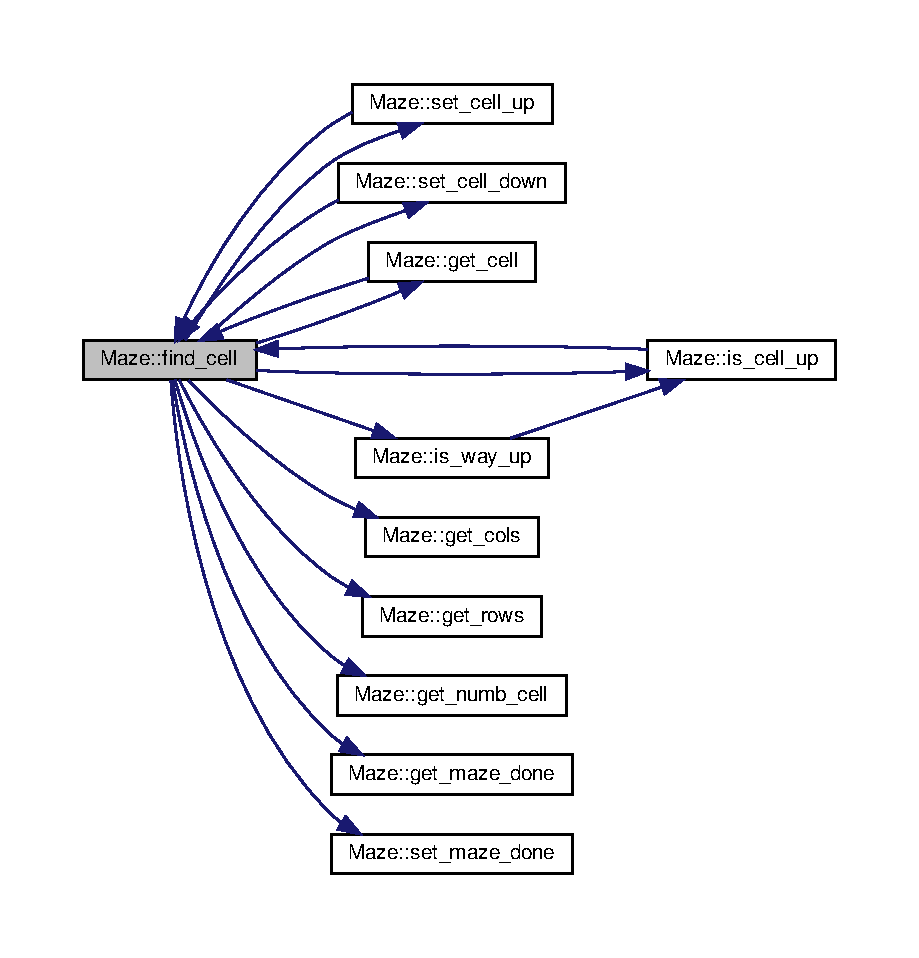
\includegraphics[width=350pt]{classMaze_aa59b935dcd5f7129636cea6e40882c56_cgraph}
\end{center}
\end{figure}
Here is the caller graph for this function\+:\nopagebreak
\begin{figure}[H]
\begin{center}
\leavevmode
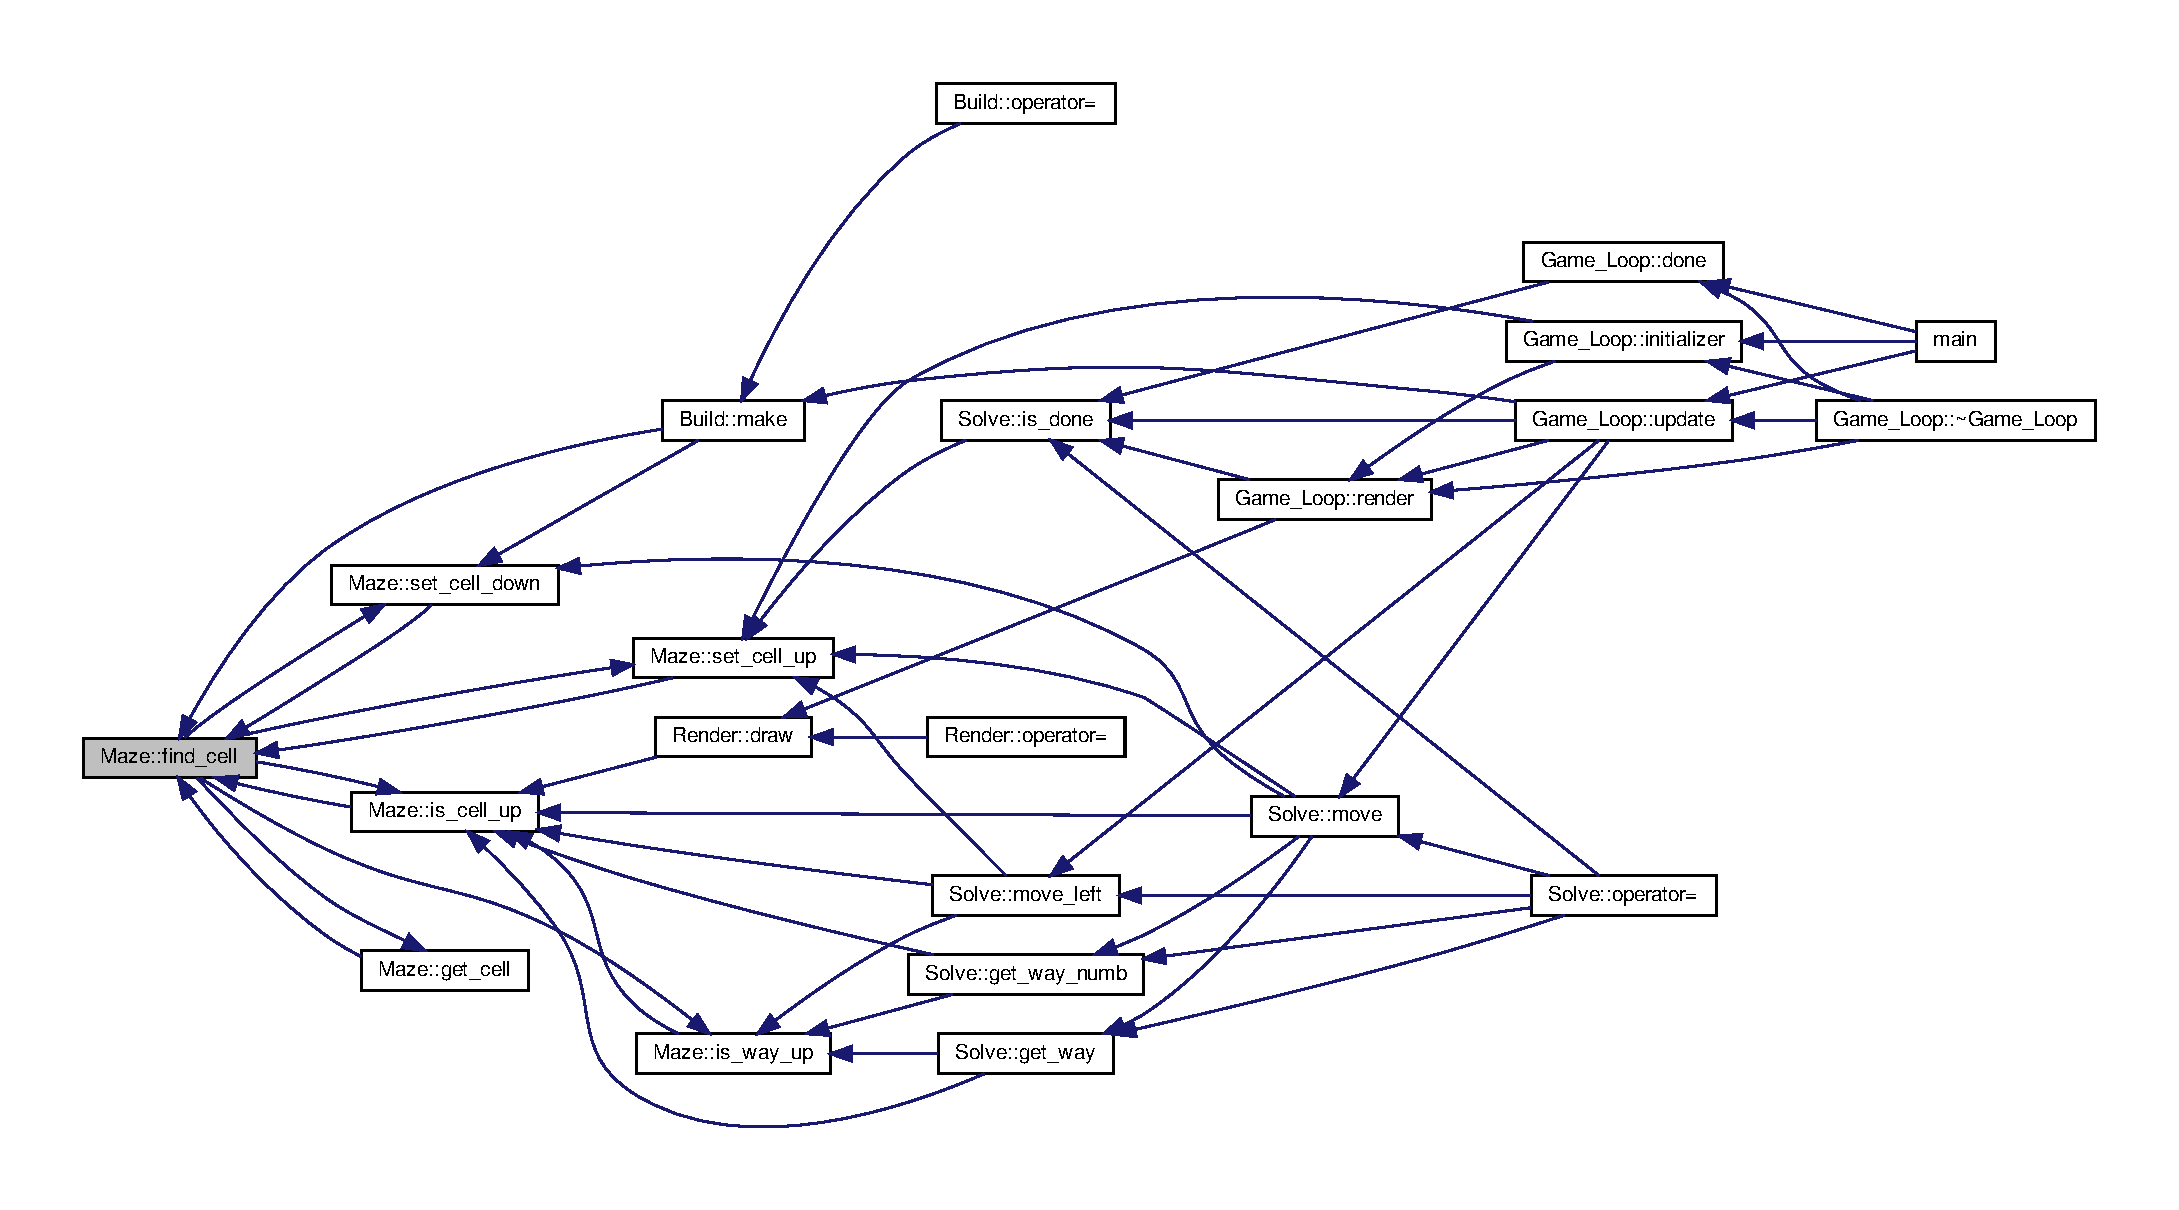
\includegraphics[width=350pt]{classMaze_aa59b935dcd5f7129636cea6e40882c56_icgraph}
\end{center}
\end{figure}
\mbox{\Hypertarget{classMaze_ae07191c6ec3cc47fce1147bc3f03a8ad}\label{classMaze_ae07191c6ec3cc47fce1147bc3f03a8ad}} 
\index{Maze@{Maze}!get\+\_\+cell@{get\+\_\+cell}}
\index{get\+\_\+cell@{get\+\_\+cell}!Maze@{Maze}}
\subsubsection{\texorpdfstring{get\+\_\+cell()}{get\_cell()}}
{\footnotesize\ttfamily \hyperlink{maze_8h_a789d352559efaa396a258805d44f4289}{bit} Maze\+::get\+\_\+cell (\begin{DoxyParamCaption}\item[{int}]{x,  }\item[{int}]{y }\end{DoxyParamCaption})}



Method to see all status of cell. 


\begin{DoxyParams}{Parameters}
{\em int} & x Coordinates X. \\
\hline
{\em int} & y Coordinates Y. \\
\hline
\end{DoxyParams}
\begin{DoxyReturn}{Returns}
return byte them corresponding the cell. 
\end{DoxyReturn}

\begin{DoxyCode}
38 \{
39     \textcolor{keywordflow}{return} m\_cell\_list[  \hyperlink{classMaze_aa59b935dcd5f7129636cea6e40882c56}{find\_cell}(y,x)  ];
40 \}
\end{DoxyCode}
Here is the call graph for this function\+:\nopagebreak
\begin{figure}[H]
\begin{center}
\leavevmode
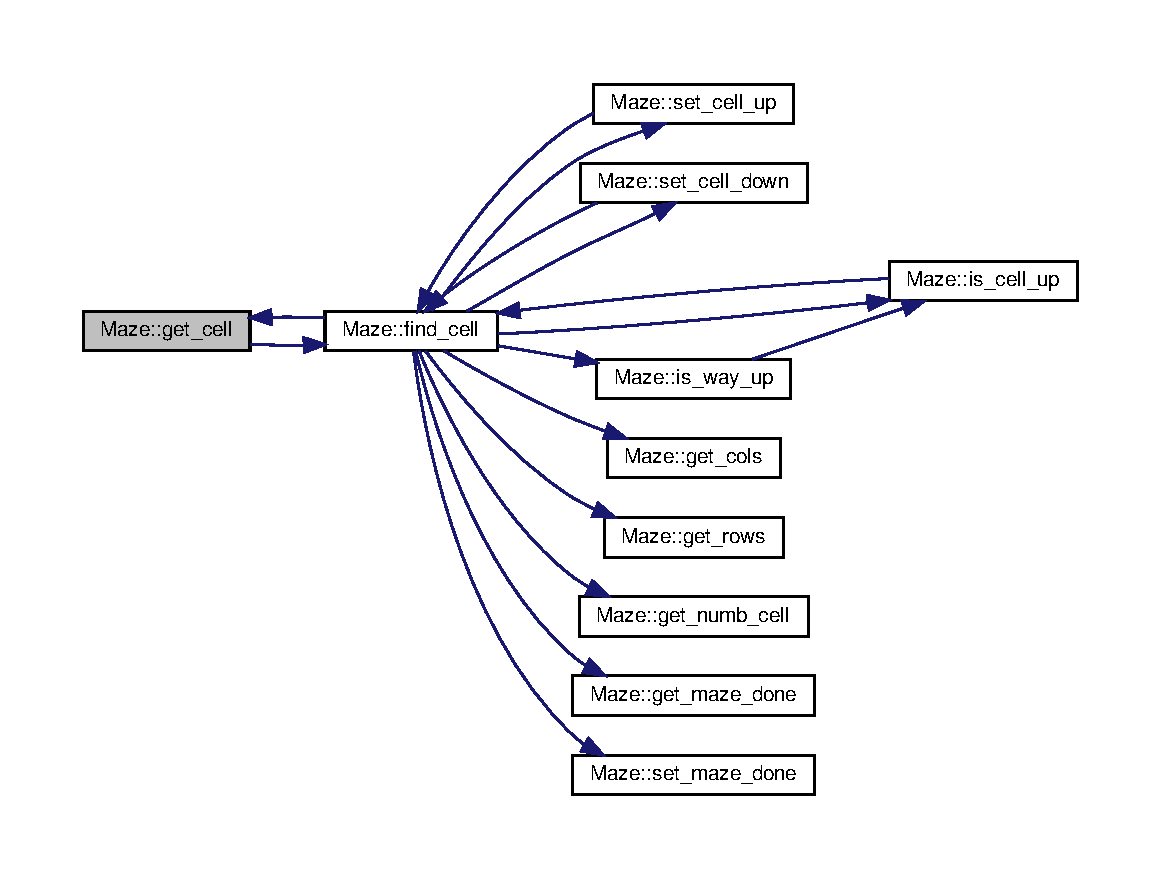
\includegraphics[width=350pt]{classMaze_ae07191c6ec3cc47fce1147bc3f03a8ad_cgraph}
\end{center}
\end{figure}
Here is the caller graph for this function\+:\nopagebreak
\begin{figure}[H]
\begin{center}
\leavevmode
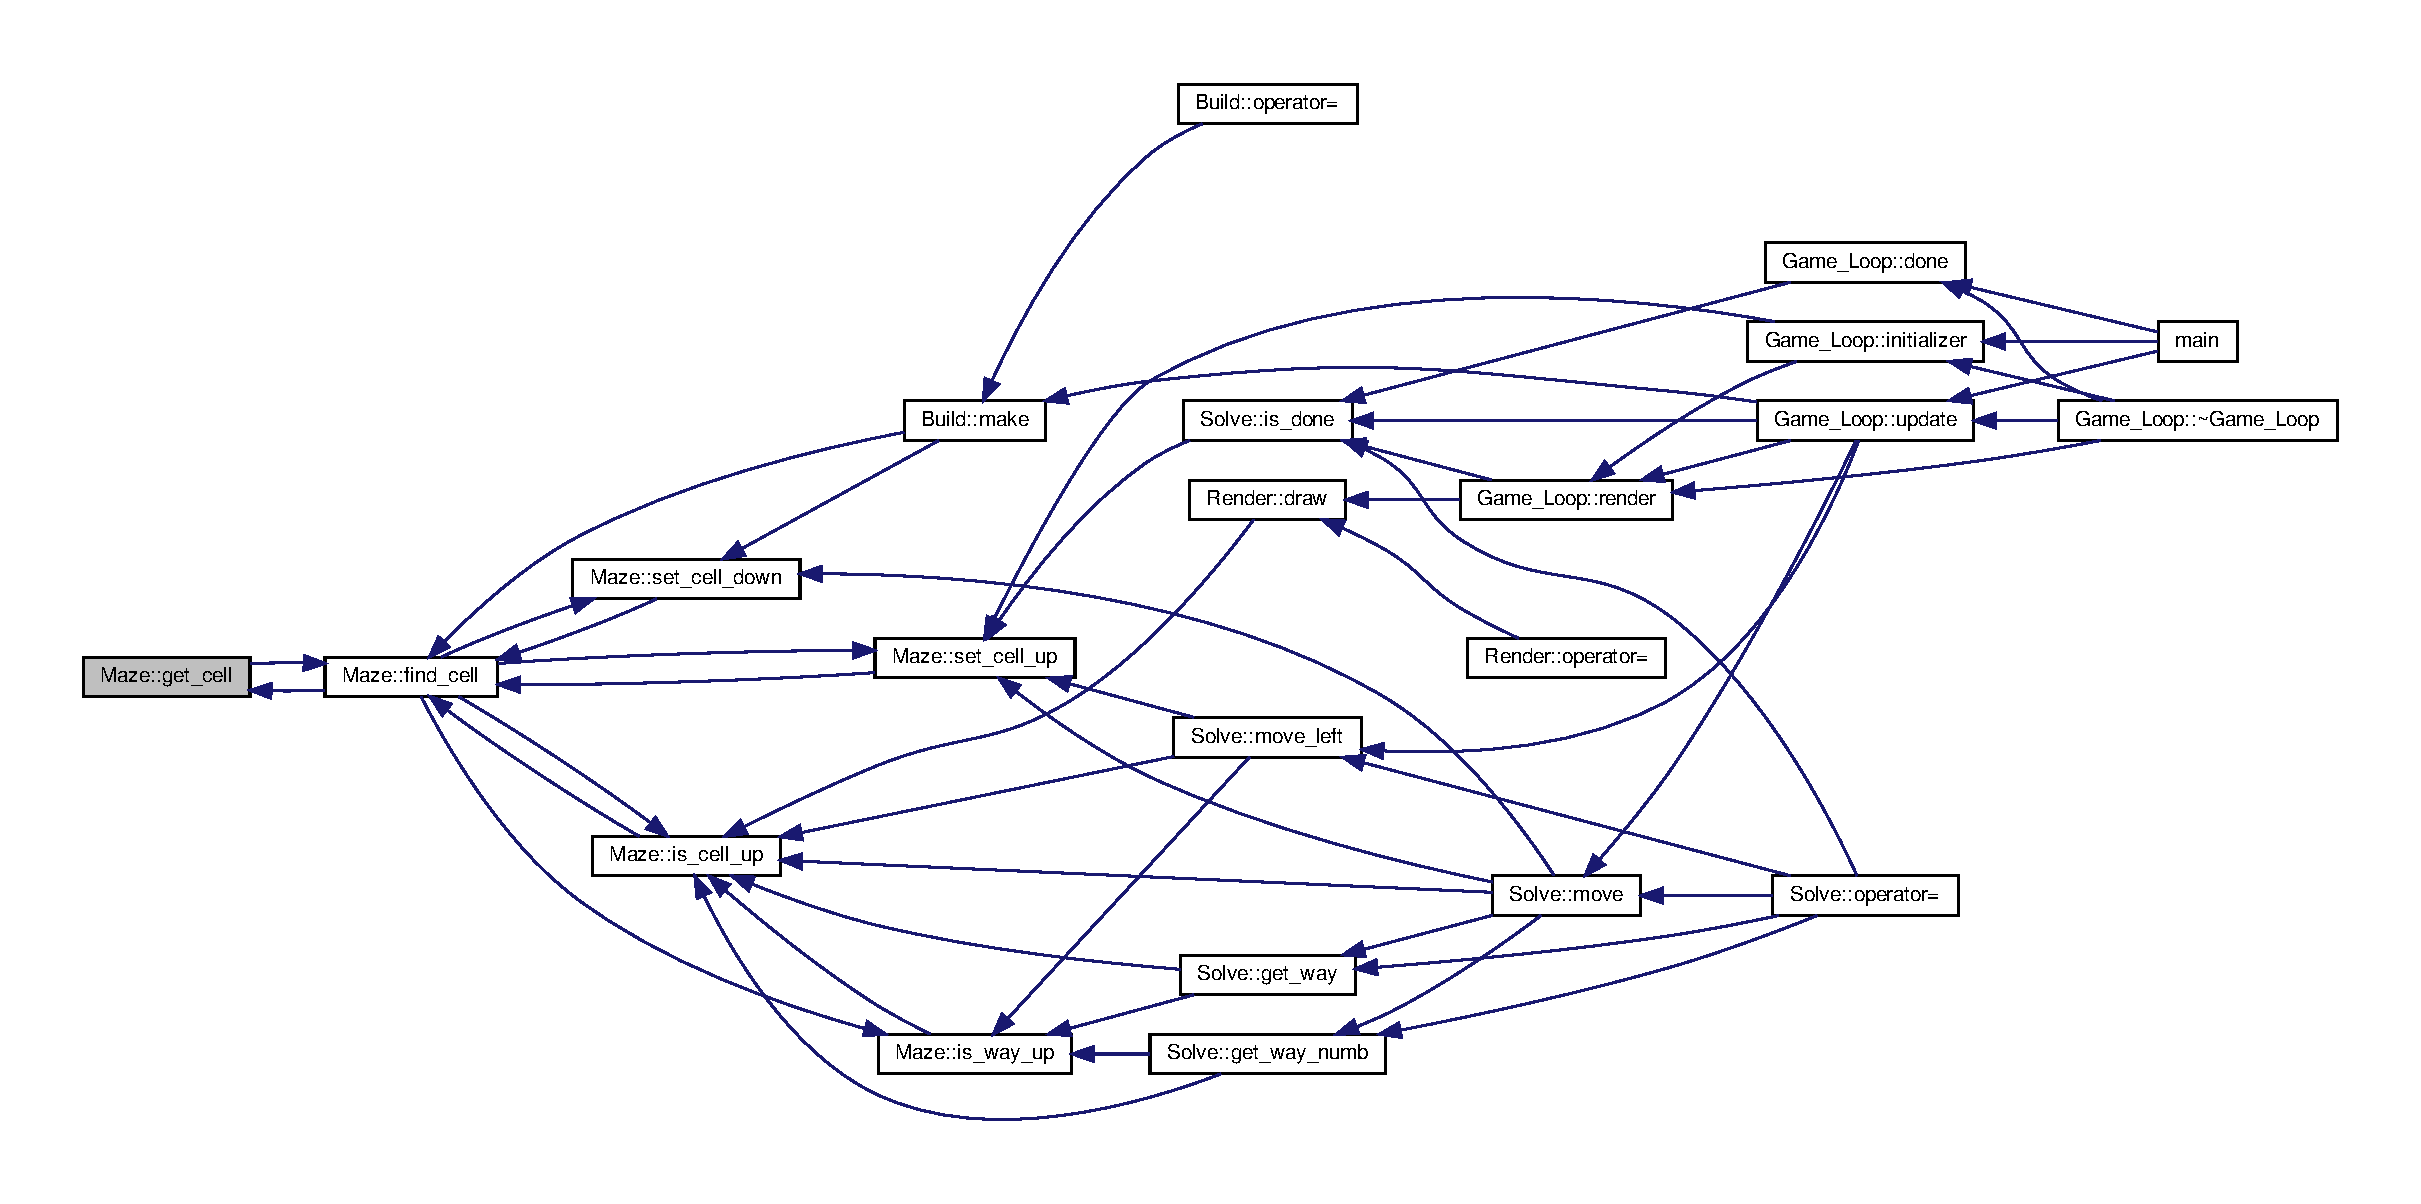
\includegraphics[width=350pt]{classMaze_ae07191c6ec3cc47fce1147bc3f03a8ad_icgraph}
\end{center}
\end{figure}
\mbox{\Hypertarget{classMaze_a8a04cd1335e96a80358181afa164d4c9}\label{classMaze_a8a04cd1335e96a80358181afa164d4c9}} 
\index{Maze@{Maze}!get\+\_\+cols@{get\+\_\+cols}}
\index{get\+\_\+cols@{get\+\_\+cols}!Maze@{Maze}}
\subsubsection{\texorpdfstring{get\+\_\+cols()}{get\_cols()}}
{\footnotesize\ttfamily int Maze\+::get\+\_\+cols (\begin{DoxyParamCaption}\item[{void}]{ }\end{DoxyParamCaption})}



Method to get numbers of colums. 

\begin{DoxyReturn}{Returns}
numbers of cols 
\end{DoxyReturn}

\begin{DoxyCode}
4 \{ \textcolor{keywordflow}{return} m\_cols; \};
\end{DoxyCode}
Here is the caller graph for this function\+:\nopagebreak
\begin{figure}[H]
\begin{center}
\leavevmode
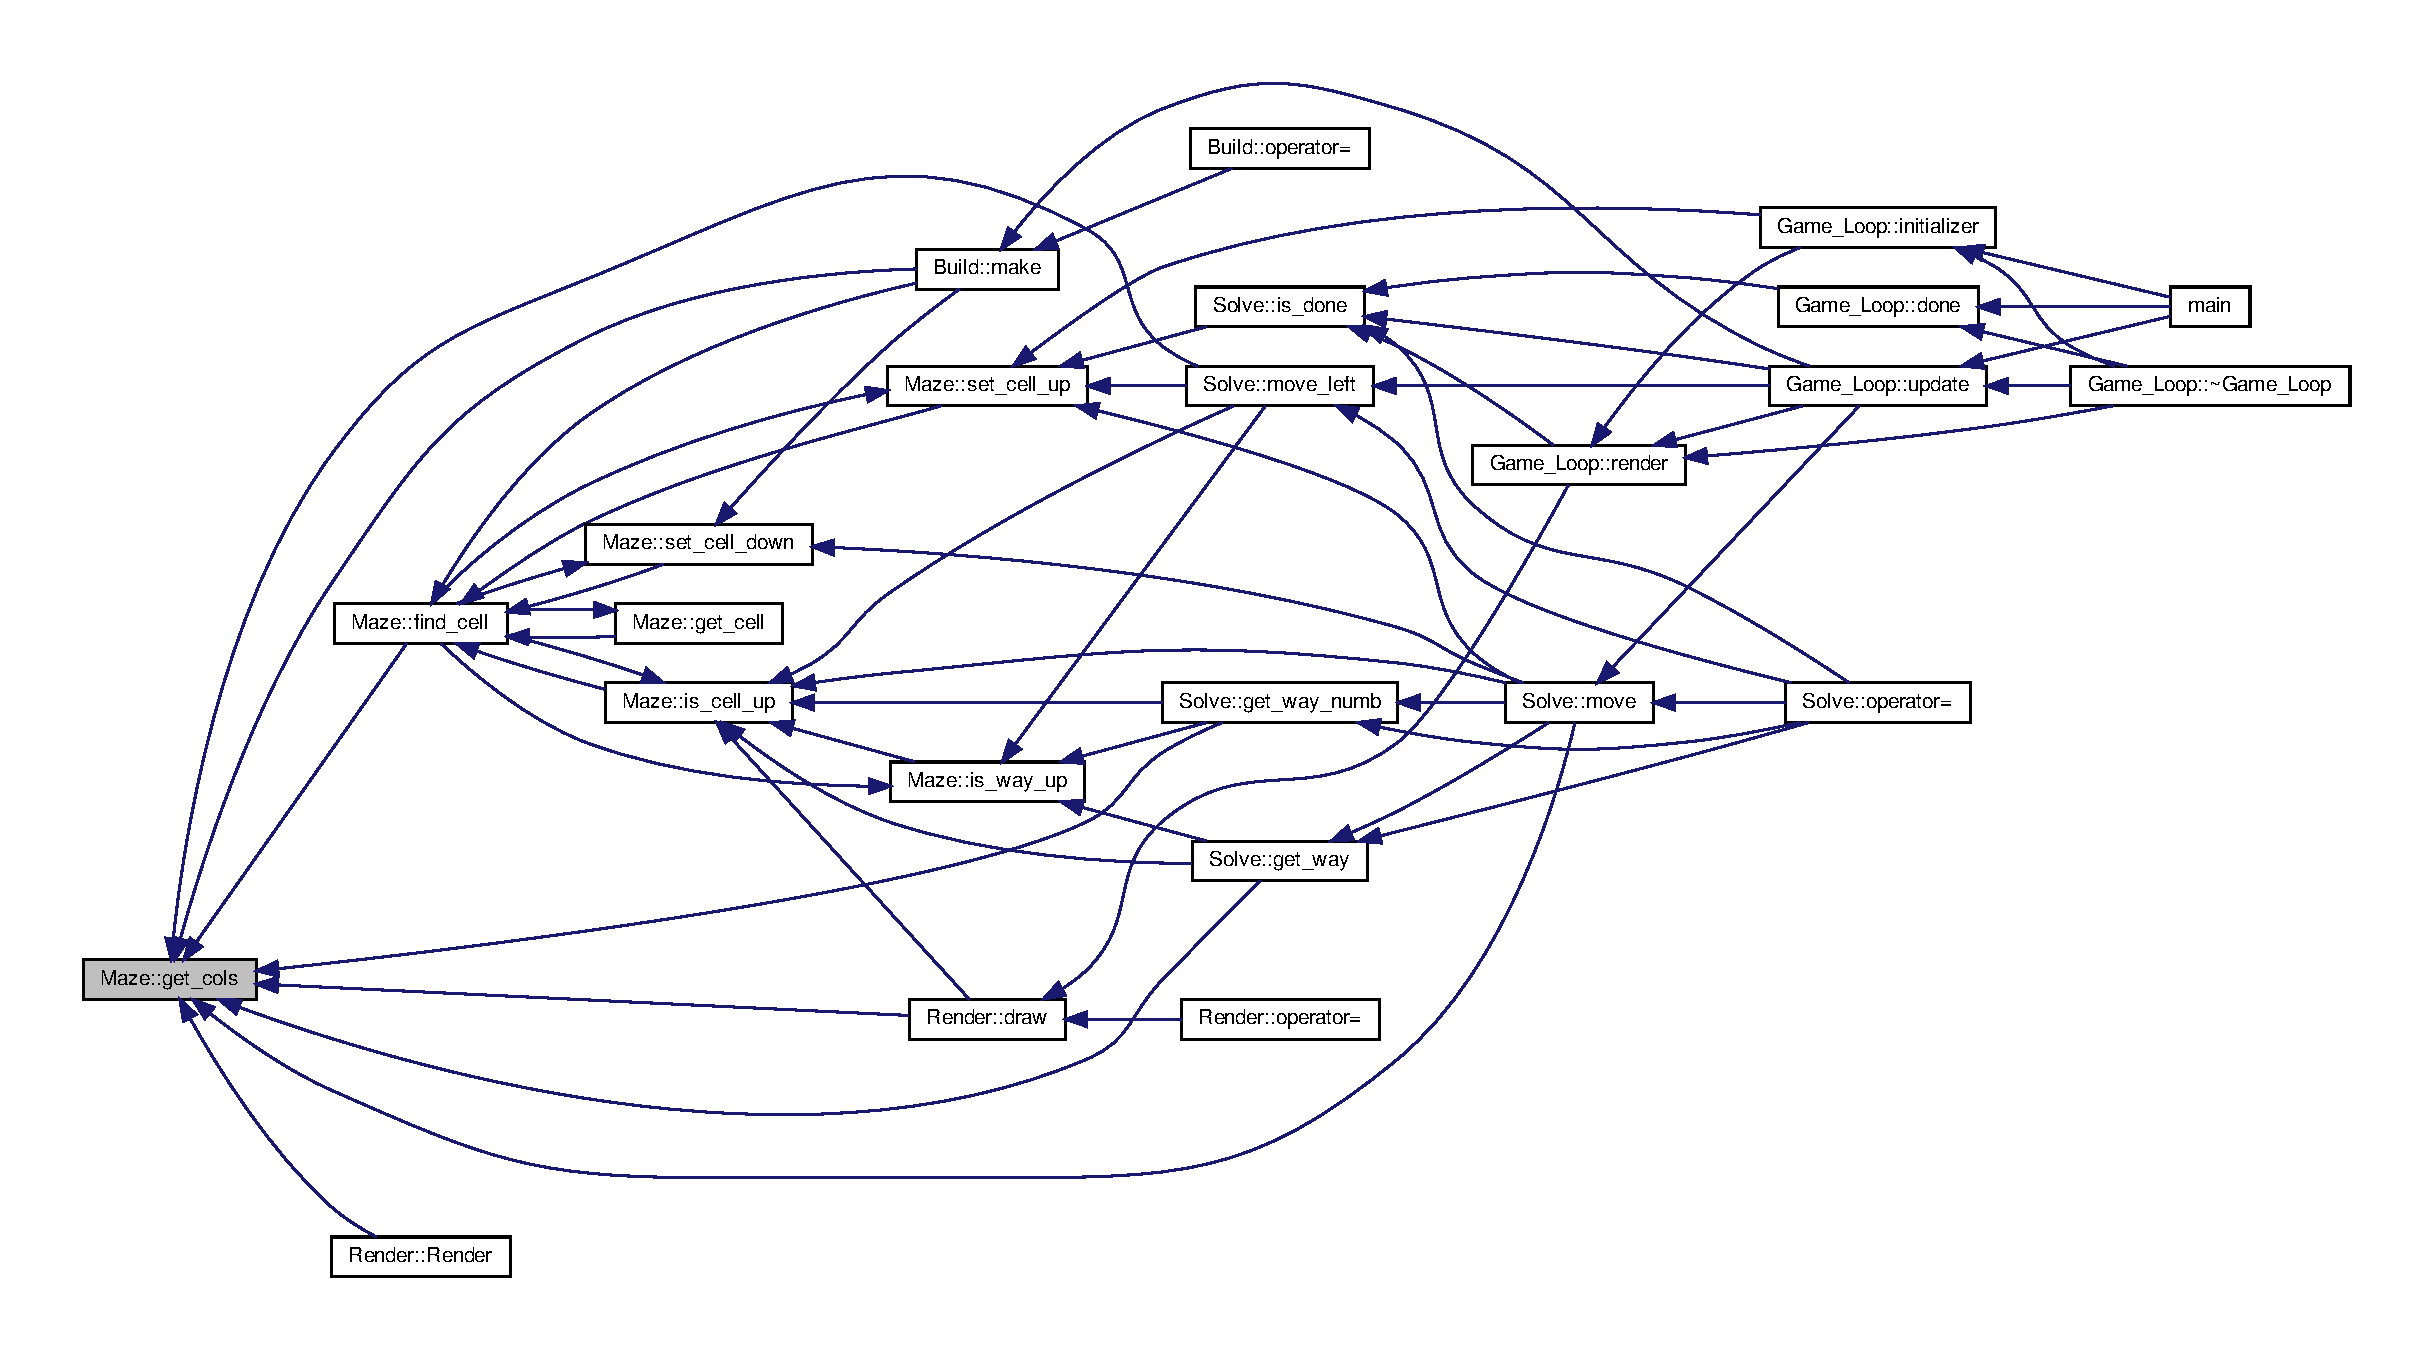
\includegraphics[width=350pt]{classMaze_a8a04cd1335e96a80358181afa164d4c9_icgraph}
\end{center}
\end{figure}
\mbox{\Hypertarget{classMaze_a152979999dd4c75014d65bf6deb5a00c}\label{classMaze_a152979999dd4c75014d65bf6deb5a00c}} 
\index{Maze@{Maze}!get\+\_\+maze\+\_\+done@{get\+\_\+maze\+\_\+done}}
\index{get\+\_\+maze\+\_\+done@{get\+\_\+maze\+\_\+done}!Maze@{Maze}}
\subsubsection{\texorpdfstring{get\+\_\+maze\+\_\+done()}{get\_maze\_done()}}
{\footnotesize\ttfamily int Maze\+::get\+\_\+maze\+\_\+done (\begin{DoxyParamCaption}\item[{void}]{ }\end{DoxyParamCaption})}


\begin{DoxyCode}
10 \{ \textcolor{keywordflow}{return} m\_maze\_done; \}
\end{DoxyCode}
Here is the caller graph for this function\+:\nopagebreak
\begin{figure}[H]
\begin{center}
\leavevmode
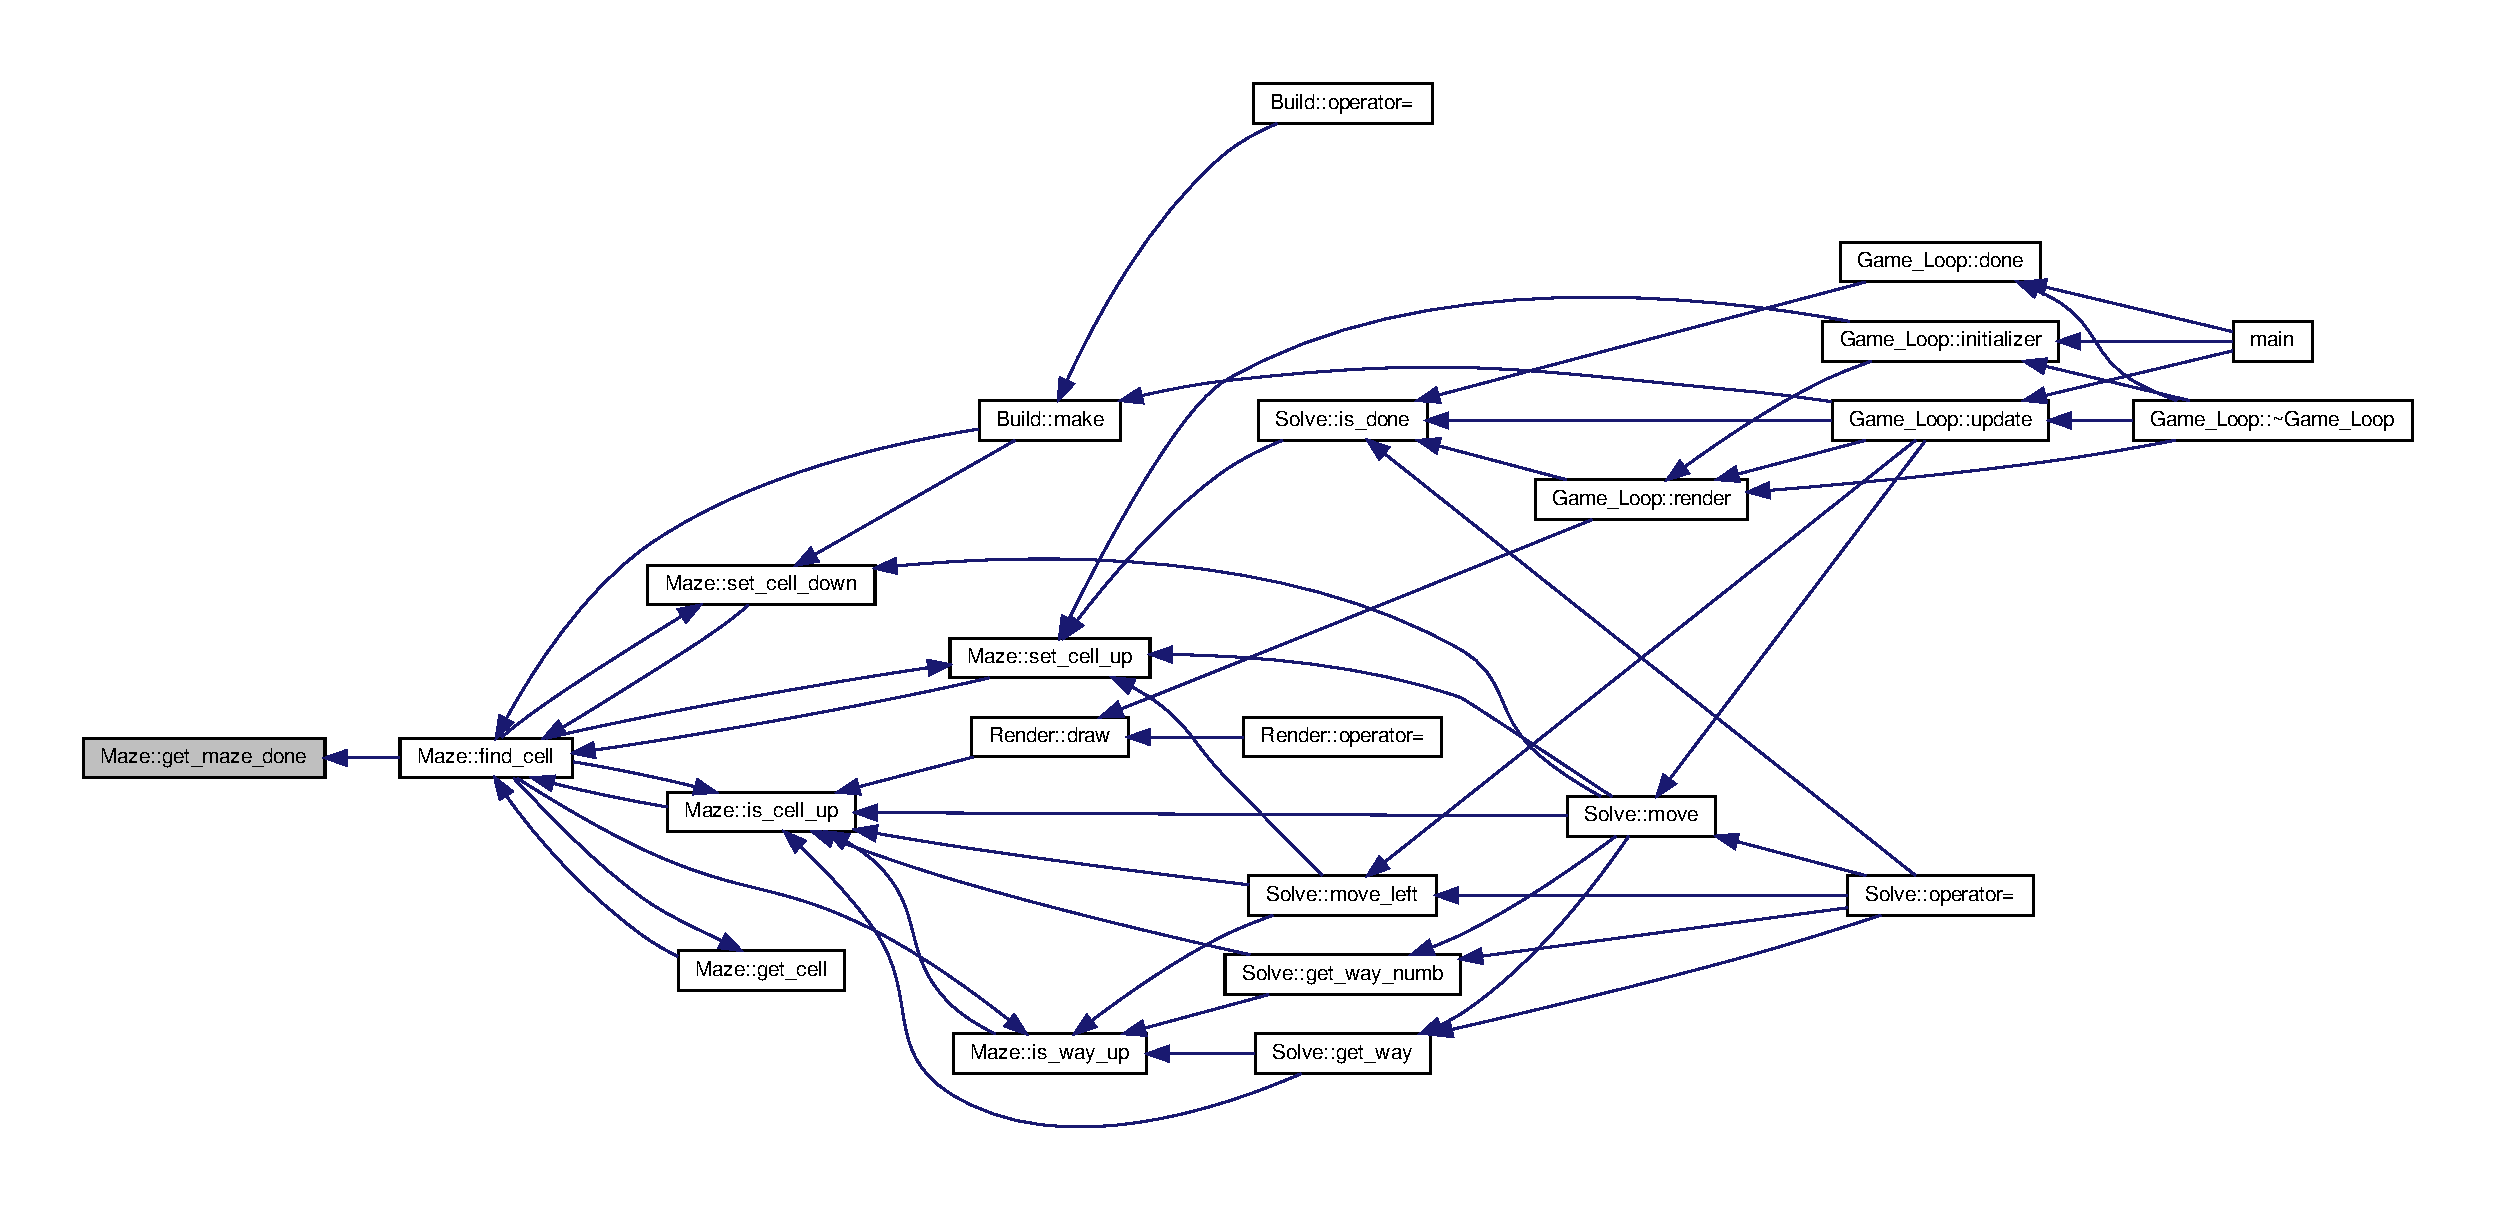
\includegraphics[width=350pt]{classMaze_a152979999dd4c75014d65bf6deb5a00c_icgraph}
\end{center}
\end{figure}
\mbox{\Hypertarget{classMaze_a90f5c1c140a9991942204d4a7fec3bf8}\label{classMaze_a90f5c1c140a9991942204d4a7fec3bf8}} 
\index{Maze@{Maze}!get\+\_\+numb\+\_\+cell@{get\+\_\+numb\+\_\+cell}}
\index{get\+\_\+numb\+\_\+cell@{get\+\_\+numb\+\_\+cell}!Maze@{Maze}}
\subsubsection{\texorpdfstring{get\+\_\+numb\+\_\+cell()}{get\_numb\_cell()}}
{\footnotesize\ttfamily int Maze\+::get\+\_\+numb\+\_\+cell (\begin{DoxyParamCaption}\item[{void}]{ }\end{DoxyParamCaption})}



Method to get numbers of cell. 

\begin{DoxyReturn}{Returns}
numbers of cell(rows$\ast$cols) 
\end{DoxyReturn}

\begin{DoxyCode}
8 \{ \textcolor{keywordflow}{return} m\_cols*m\_rows; \}
\end{DoxyCode}
Here is the caller graph for this function\+:\nopagebreak
\begin{figure}[H]
\begin{center}
\leavevmode
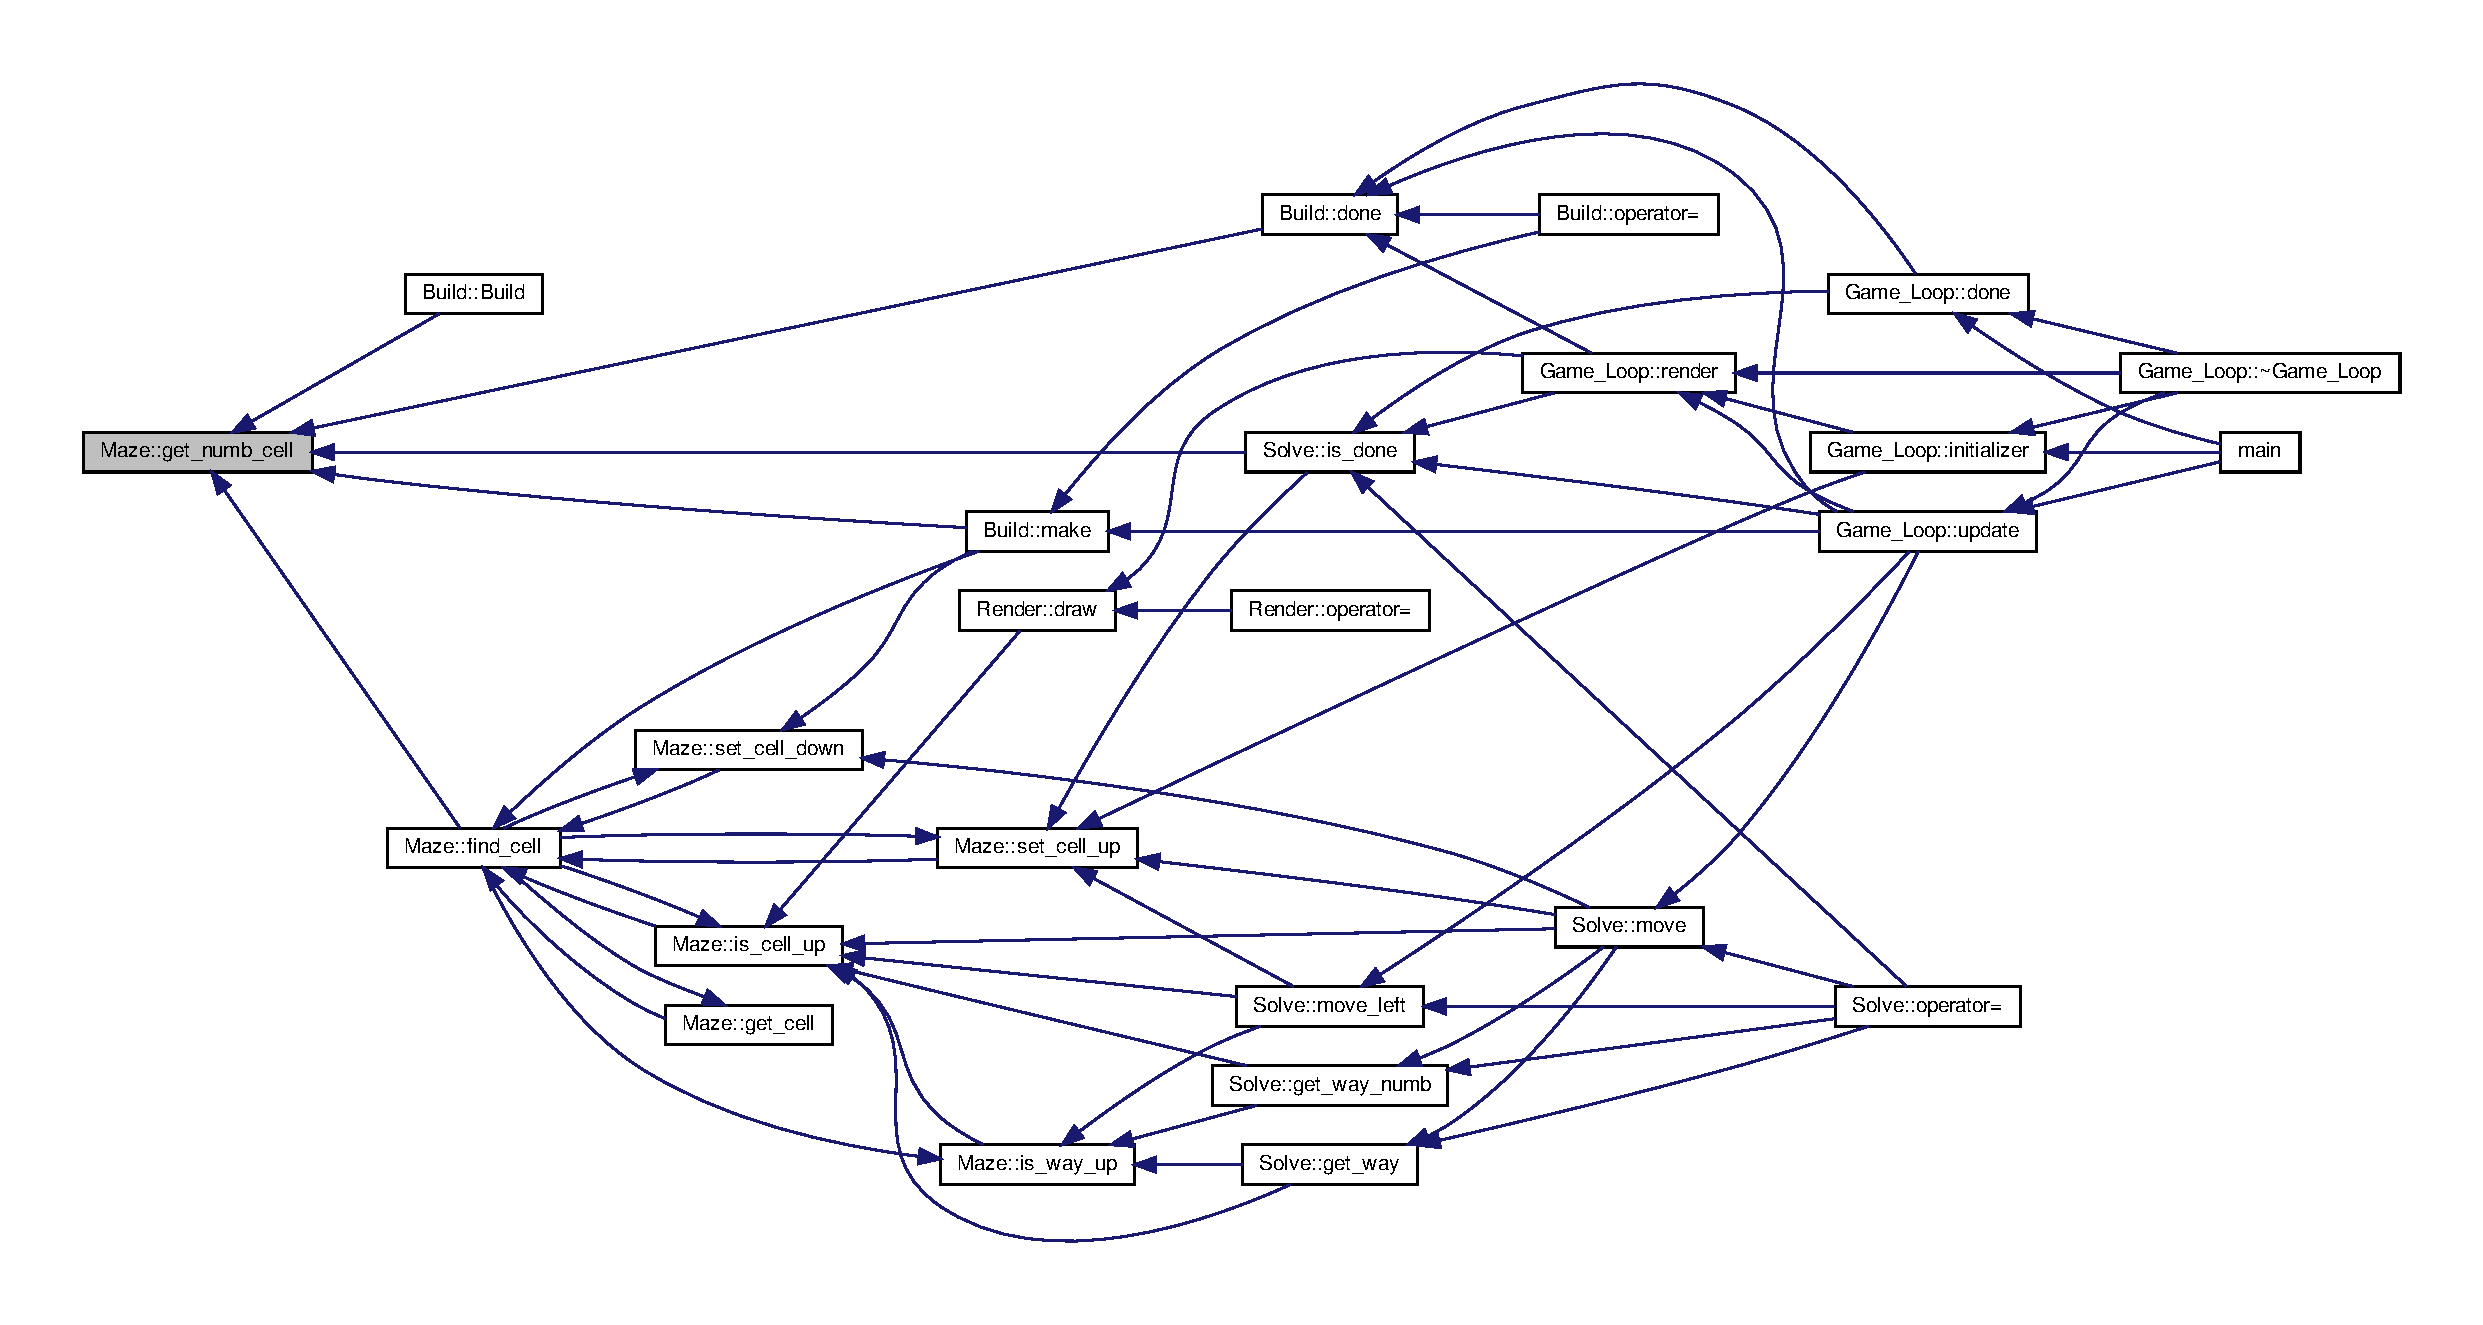
\includegraphics[width=350pt]{classMaze_a90f5c1c140a9991942204d4a7fec3bf8_icgraph}
\end{center}
\end{figure}
\mbox{\Hypertarget{classMaze_ac786606a34632b2254b2d27d5f5f0f3f}\label{classMaze_ac786606a34632b2254b2d27d5f5f0f3f}} 
\index{Maze@{Maze}!get\+\_\+rows@{get\+\_\+rows}}
\index{get\+\_\+rows@{get\+\_\+rows}!Maze@{Maze}}
\subsubsection{\texorpdfstring{get\+\_\+rows()}{get\_rows()}}
{\footnotesize\ttfamily int Maze\+::get\+\_\+rows (\begin{DoxyParamCaption}\item[{void}]{ }\end{DoxyParamCaption})}



Method to get numbers of rows. 

\begin{DoxyReturn}{Returns}
numbers of rows 
\end{DoxyReturn}

\begin{DoxyCode}
6 \{ \textcolor{keywordflow}{return} m\_rows; \};
\end{DoxyCode}
Here is the caller graph for this function\+:\nopagebreak
\begin{figure}[H]
\begin{center}
\leavevmode
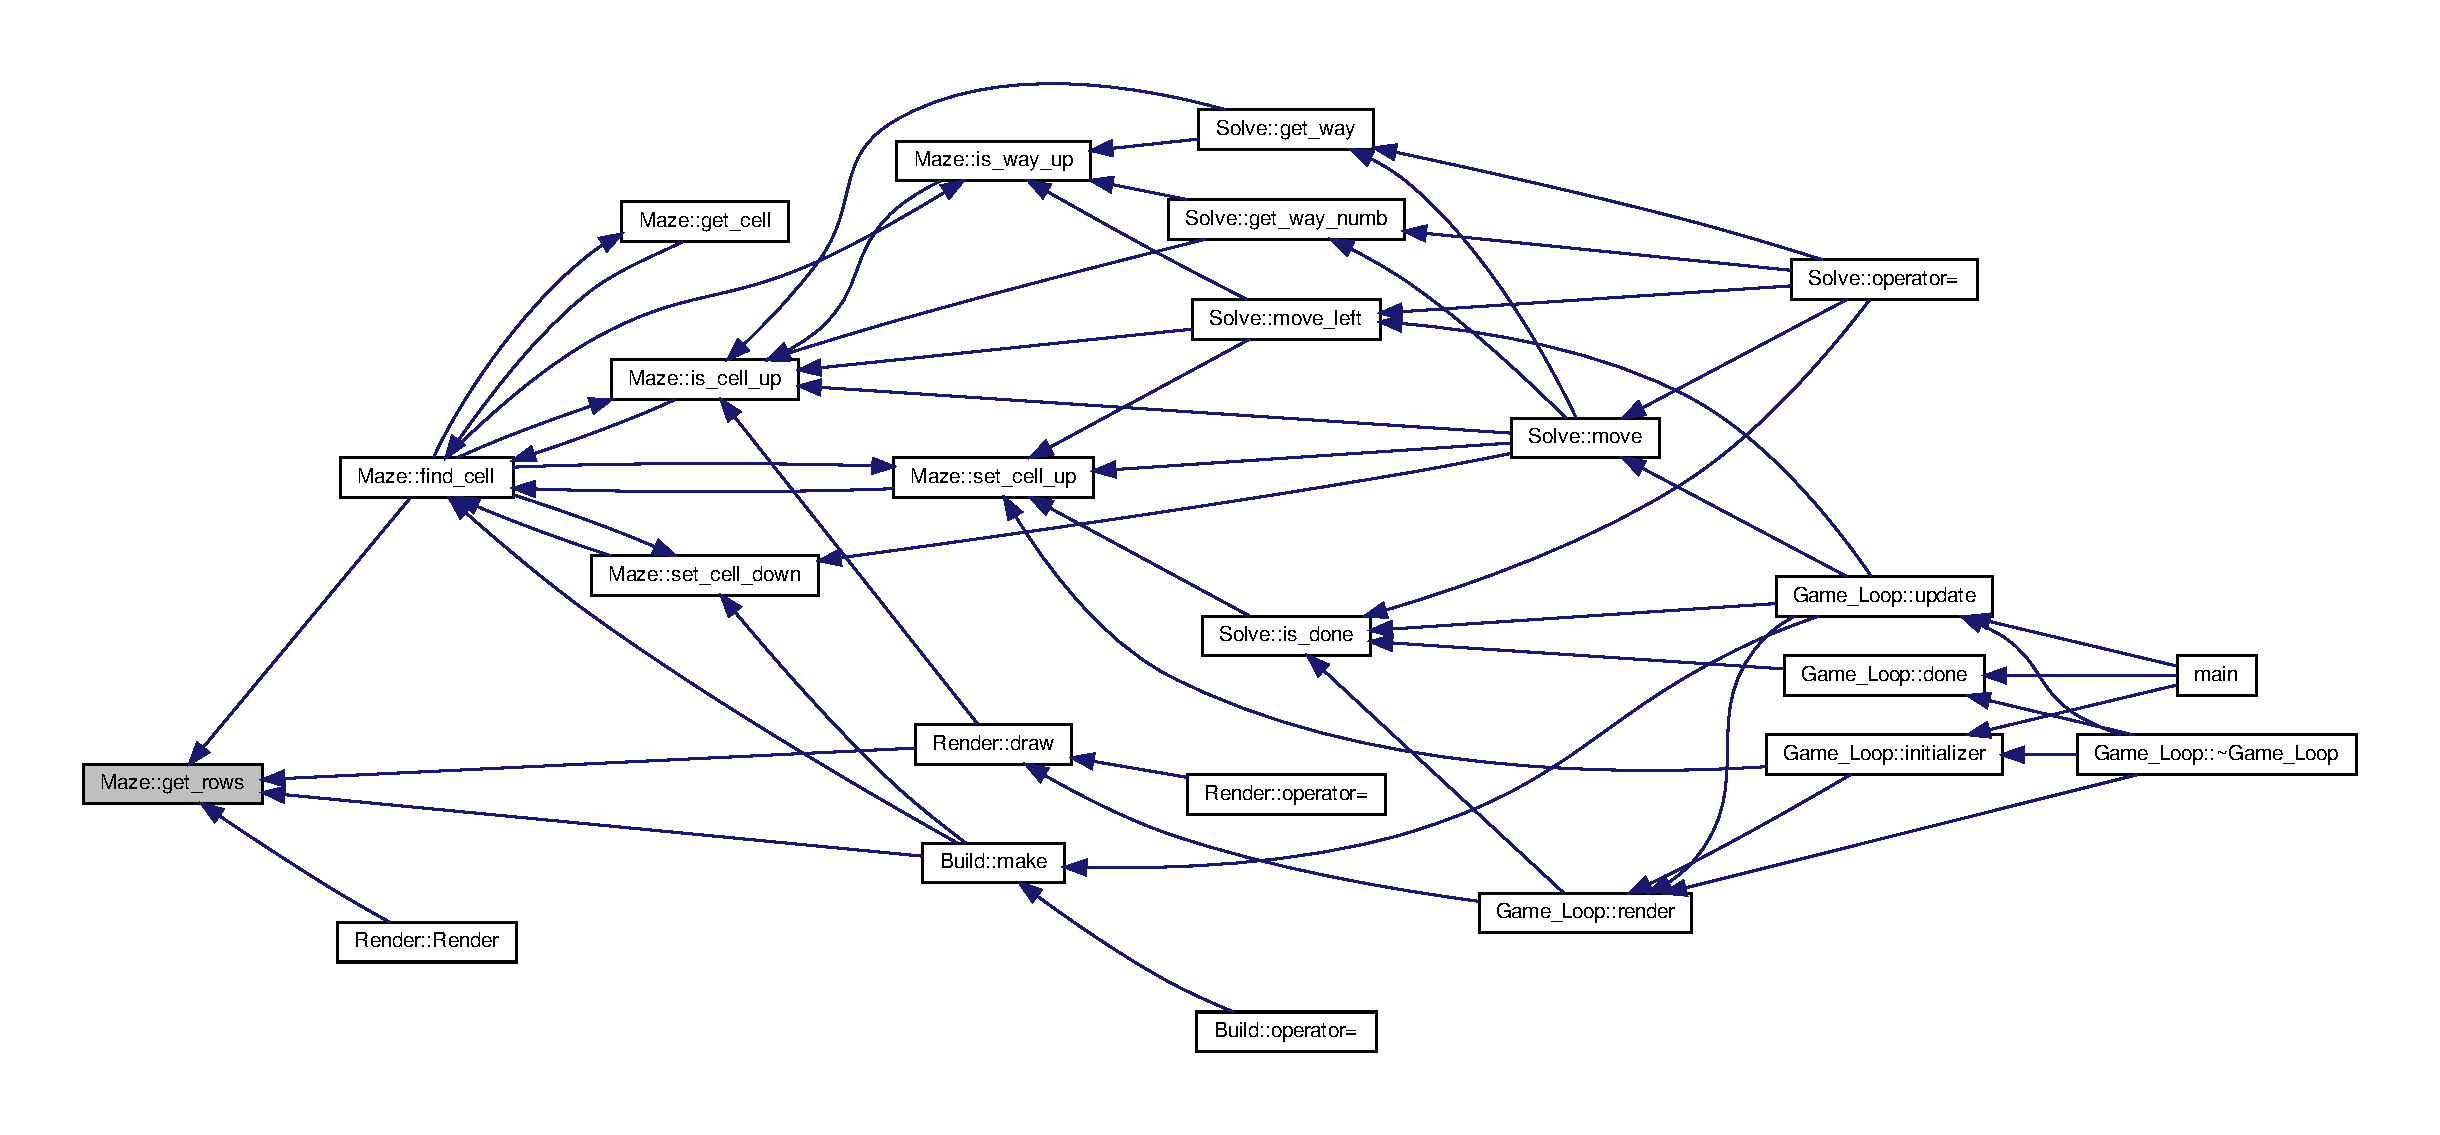
\includegraphics[width=350pt]{classMaze_ac786606a34632b2254b2d27d5f5f0f3f_icgraph}
\end{center}
\end{figure}
\mbox{\Hypertarget{classMaze_a2b0e69e72d6c3e1037578f057946a21e}\label{classMaze_a2b0e69e72d6c3e1037578f057946a21e}} 
\index{Maze@{Maze}!is\+\_\+cell\+\_\+up@{is\+\_\+cell\+\_\+up}}
\index{is\+\_\+cell\+\_\+up@{is\+\_\+cell\+\_\+up}!Maze@{Maze}}
\subsubsection{\texorpdfstring{is\+\_\+cell\+\_\+up()}{is\_cell\_up()}\hspace{0.1cm}{\footnotesize\ttfamily [1/2]}}
{\footnotesize\ttfamily bool Maze\+::is\+\_\+cell\+\_\+up (\begin{DoxyParamCaption}\item[{int}]{x,  }\item[{int}]{y,  }\item[{\hyperlink{classMaze_a07167e321eac2b67100fb82ecb98f1d1}{status\+\_\+cell}}]{sc }\end{DoxyParamCaption})}



Method to check if the status cell sc is up. 


\begin{DoxyParams}{Parameters}
{\em int} & x Coordinates X. \\
\hline
{\em int} & y Coordinates Y. \\
\hline
{\em status\+\_\+cell} & sc status to be check. \\
\hline
\end{DoxyParams}
\begin{DoxyReturn}{Returns}
True if is up otherwise False 
\end{DoxyReturn}

\begin{DoxyCode}
43 \{
44     \textcolor{keywordflow}{if}((\hyperlink{maze_8h_a789d352559efaa396a258805d44f4289}{bit})sc == (m\_cell\_list[ \hyperlink{classMaze_aa59b935dcd5f7129636cea6e40882c56}{find\_cell}(y,x) ] & (\hyperlink{maze_8h_a789d352559efaa396a258805d44f4289}{bit})sc) ) \textcolor{keywordflow}{return} \textcolor{keyword}{true};
45 
46     \textcolor{keywordflow}{return} \textcolor{keyword}{false};
47 \}
\end{DoxyCode}
Here is the call graph for this function\+:\nopagebreak
\begin{figure}[H]
\begin{center}
\leavevmode
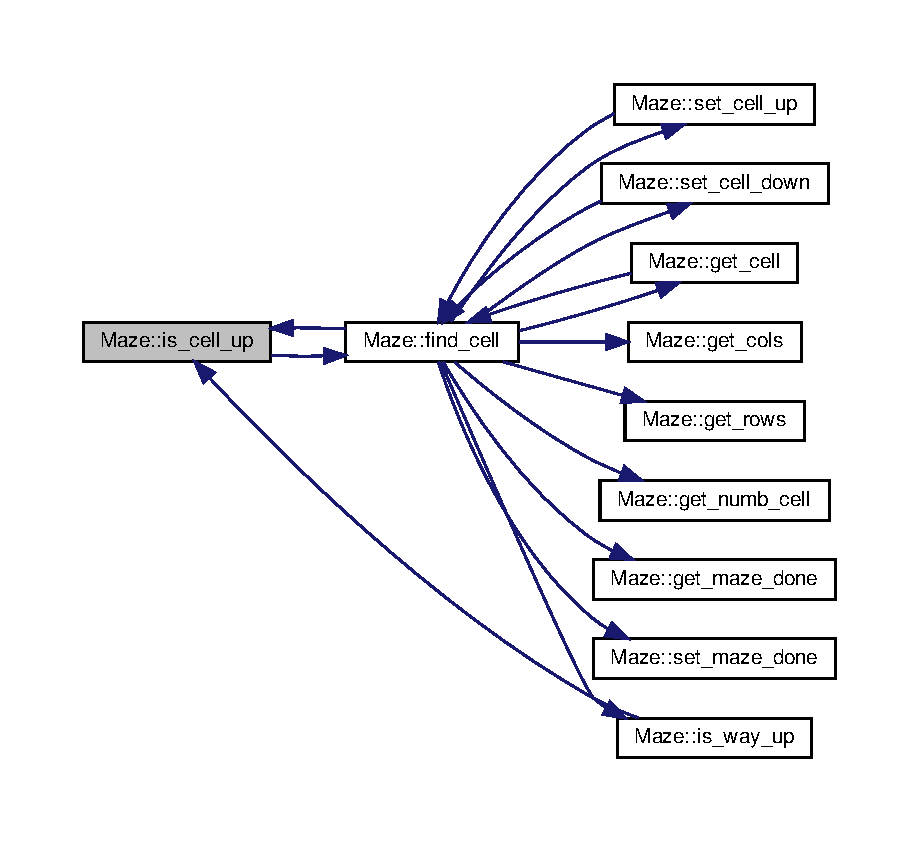
\includegraphics[width=350pt]{classMaze_a2b0e69e72d6c3e1037578f057946a21e_cgraph}
\end{center}
\end{figure}
Here is the caller graph for this function\+:\nopagebreak
\begin{figure}[H]
\begin{center}
\leavevmode
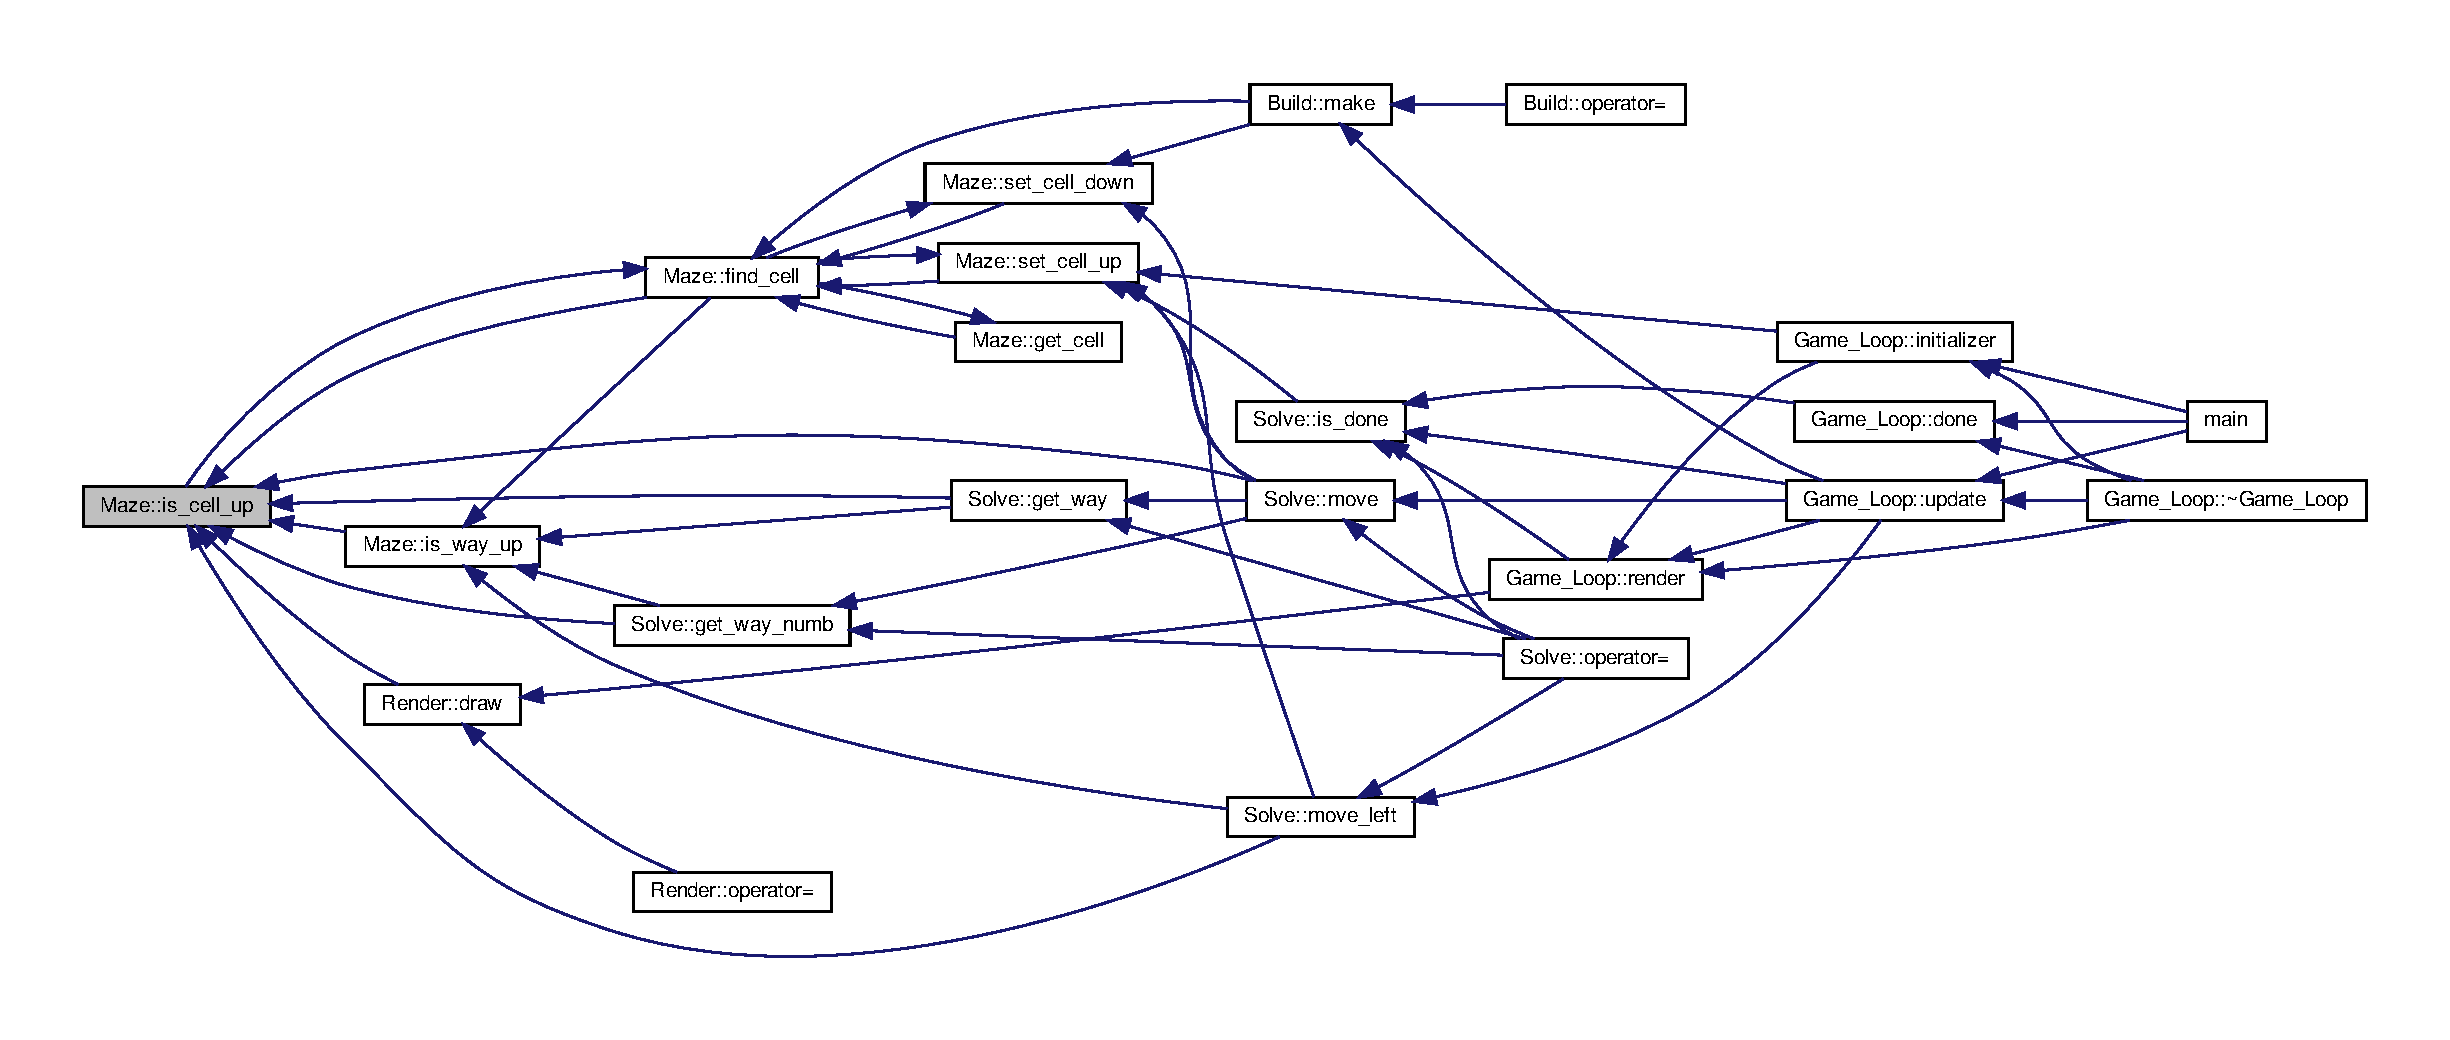
\includegraphics[width=350pt]{classMaze_a2b0e69e72d6c3e1037578f057946a21e_icgraph}
\end{center}
\end{figure}
\mbox{\Hypertarget{classMaze_ad5dd6a918e4fd4bb6392e0a0bc08b81d}\label{classMaze_ad5dd6a918e4fd4bb6392e0a0bc08b81d}} 
\index{Maze@{Maze}!is\+\_\+cell\+\_\+up@{is\+\_\+cell\+\_\+up}}
\index{is\+\_\+cell\+\_\+up@{is\+\_\+cell\+\_\+up}!Maze@{Maze}}
\subsubsection{\texorpdfstring{is\+\_\+cell\+\_\+up()}{is\_cell\_up()}\hspace{0.1cm}{\footnotesize\ttfamily [2/2]}}
{\footnotesize\ttfamily bool Maze\+::is\+\_\+cell\+\_\+up (\begin{DoxyParamCaption}\item[{int}]{cell,  }\item[{\hyperlink{classMaze_a07167e321eac2b67100fb82ecb98f1d1}{status\+\_\+cell}}]{sc }\end{DoxyParamCaption})}



Method to check if the status cell sc is up. 


\begin{DoxyParams}{Parameters}
{\em int} & Cell of the vector. \\
\hline
{\em status\+\_\+cell} & sc status to be check. \\
\hline
\end{DoxyParams}
\begin{DoxyReturn}{Returns}
True if is up otherwise False 
\end{DoxyReturn}

\begin{DoxyCode}
50 \{
51     \textcolor{keywordflow}{if}((\hyperlink{maze_8h_a789d352559efaa396a258805d44f4289}{bit})sc == (m\_cell\_list[ cell ] & (\hyperlink{maze_8h_a789d352559efaa396a258805d44f4289}{bit})sc) ) \textcolor{keywordflow}{return} \textcolor{keyword}{true};
52 
53     \textcolor{keywordflow}{return} \textcolor{keyword}{false};
54 \}
\end{DoxyCode}
\mbox{\Hypertarget{classMaze_a308fa695665de6217c0e7f28aab5adda}\label{classMaze_a308fa695665de6217c0e7f28aab5adda}} 
\index{Maze@{Maze}!is\+\_\+way\+\_\+up@{is\+\_\+way\+\_\+up}}
\index{is\+\_\+way\+\_\+up@{is\+\_\+way\+\_\+up}!Maze@{Maze}}
\subsubsection{\texorpdfstring{is\+\_\+way\+\_\+up()}{is\_way\_up()}}
{\footnotesize\ttfamily bool Maze\+::is\+\_\+way\+\_\+up (\begin{DoxyParamCaption}\item[{int}]{cell }\end{DoxyParamCaption})}



Method to check if the cell have be see. 


\begin{DoxyParams}{Parameters}
{\em int} & Cell of the vector. \\
\hline
\end{DoxyParams}
\begin{DoxyReturn}{Returns}
True if the cell is way our discarted otherwise False 
\end{DoxyReturn}

\begin{DoxyCode}
57 \{
58     \textcolor{keywordflow}{if}( \hyperlink{classMaze_a2b0e69e72d6c3e1037578f057946a21e}{is\_cell\_up}( cell, \hyperlink{classMaze_a07167e321eac2b67100fb82ecb98f1d1a94708897ec9db8647dfe695714c98e46}{Maze::status\_cell::discarded} ))
59     \{
60         \textcolor{keywordflow}{return} \textcolor{keyword}{true};
61     \}
62 
63     \textcolor{keywordflow}{if}( \hyperlink{classMaze_a2b0e69e72d6c3e1037578f057946a21e}{is\_cell\_up}( cell, \hyperlink{classMaze_a07167e321eac2b67100fb82ecb98f1d1ac83b72dd001482ce10f0b106c7a0ed0e}{Maze::status\_cell::way} ) )
64     \{
65         \textcolor{keywordflow}{return} \textcolor{keyword}{true};
66     \}
67 
68     \textcolor{keywordflow}{return} \textcolor{keyword}{false};
69 \}
\end{DoxyCode}
Here is the call graph for this function\+:\nopagebreak
\begin{figure}[H]
\begin{center}
\leavevmode
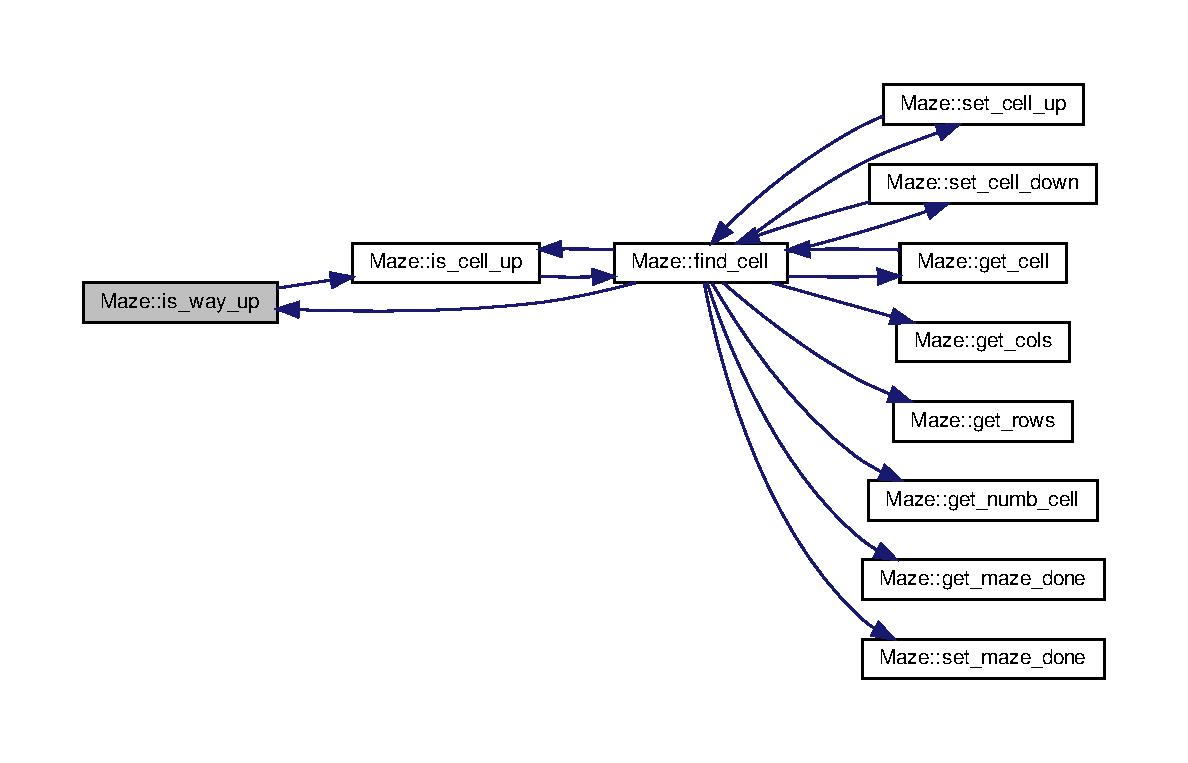
\includegraphics[width=350pt]{classMaze_a308fa695665de6217c0e7f28aab5adda_cgraph}
\end{center}
\end{figure}
Here is the caller graph for this function\+:\nopagebreak
\begin{figure}[H]
\begin{center}
\leavevmode
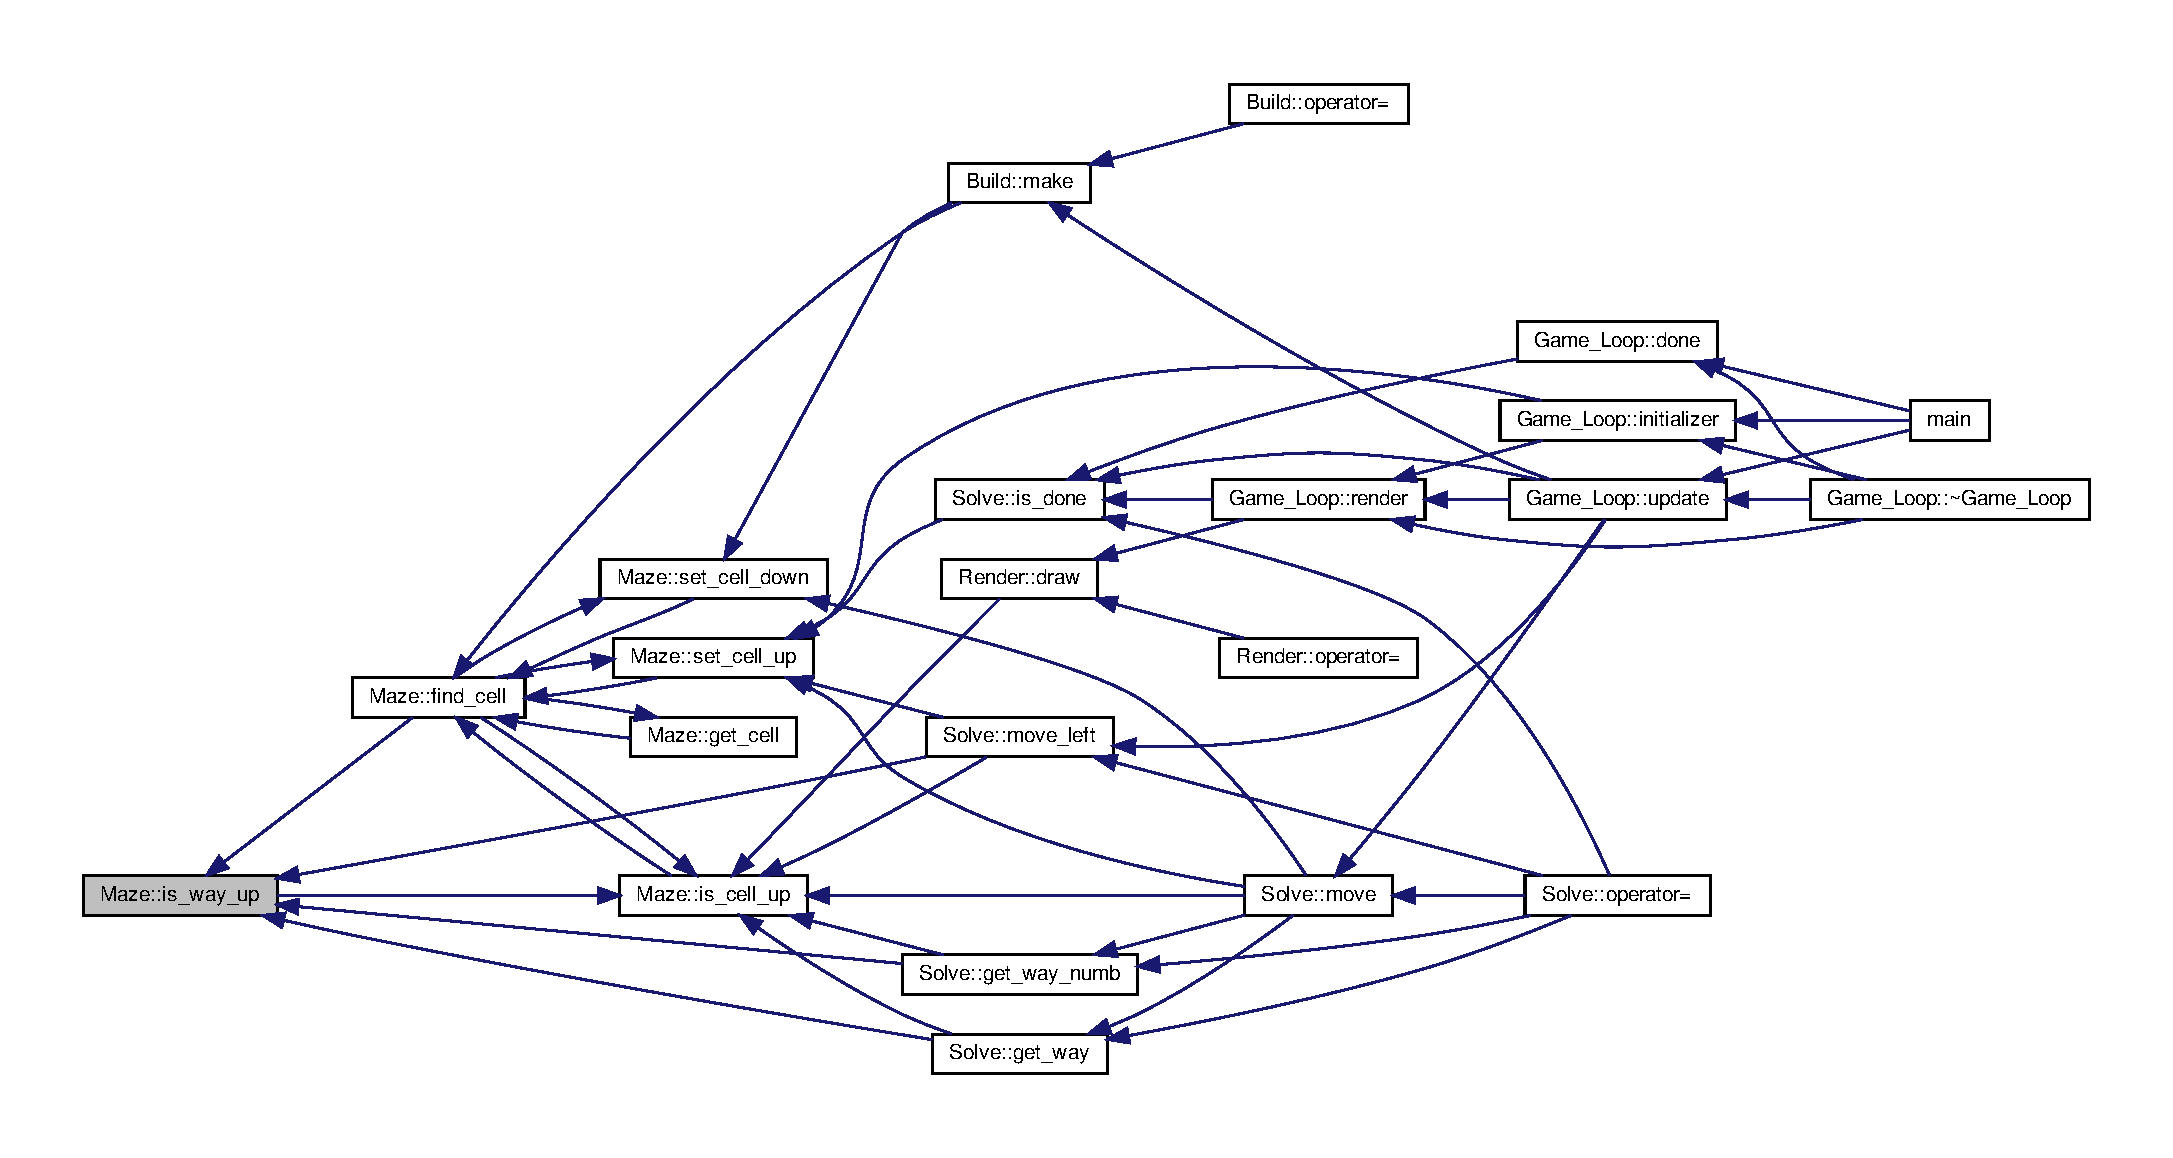
\includegraphics[width=350pt]{classMaze_a308fa695665de6217c0e7f28aab5adda_icgraph}
\end{center}
\end{figure}
\mbox{\Hypertarget{classMaze_a41468a30ae450b06d4a07304e9cda5ed}\label{classMaze_a41468a30ae450b06d4a07304e9cda5ed}} 
\index{Maze@{Maze}!operator=@{operator=}}
\index{operator=@{operator=}!Maze@{Maze}}
\subsubsection{\texorpdfstring{operator=()}{operator=()}}
{\footnotesize\ttfamily \hyperlink{classMaze}{Maze}\& Maze\+::operator= (\begin{DoxyParamCaption}\item[{const \hyperlink{classMaze}{Maze} \&}]{m }\end{DoxyParamCaption})\hspace{0.3cm}{\ttfamily [inline]}}



! Assignmentt Operator. 


\begin{DoxyCode}
66         \{
67             this->m\_cell = m.m\_cell;
68             this->m\_cell\_list = m.m\_cell\_list;
69             this->m\_cols = m.m\_cols;
70             this->m\_rows = m.m\_rows;
71             
72             \textcolor{keywordflow}{return} *\textcolor{keyword}{this};
73         \}
\end{DoxyCode}
\mbox{\Hypertarget{classMaze_ab86292a84aa56a26c4c07f4aa684d9bb}\label{classMaze_ab86292a84aa56a26c4c07f4aa684d9bb}} 
\index{Maze@{Maze}!set\+\_\+cell\+\_\+down@{set\+\_\+cell\+\_\+down}}
\index{set\+\_\+cell\+\_\+down@{set\+\_\+cell\+\_\+down}!Maze@{Maze}}
\subsubsection{\texorpdfstring{set\+\_\+cell\+\_\+down()}{set\_cell\_down()}\hspace{0.1cm}{\footnotesize\ttfamily [1/2]}}
{\footnotesize\ttfamily void Maze\+::set\+\_\+cell\+\_\+down (\begin{DoxyParamCaption}\item[{int}]{x,  }\item[{int}]{y,  }\item[{\hyperlink{classMaze_a07167e321eac2b67100fb82ecb98f1d1}{status\+\_\+cell}}]{sc }\end{DoxyParamCaption})}



Method to change bit corresponding status cell to zero. 


\begin{DoxyParams}{Parameters}
{\em int} & x Coordinates X. \\
\hline
{\em int} & y Coordinates Y. \\
\hline
{\em status\+\_\+cell} & sc status to be change. \\
\hline
\end{DoxyParams}

\begin{DoxyCode}
26 \{
27     m\_cell\_list[ \hyperlink{classMaze_aa59b935dcd5f7129636cea6e40882c56}{find\_cell}(y,x)] = ~m\_cell\_list[ \hyperlink{classMaze_aa59b935dcd5f7129636cea6e40882c56}{find\_cell}(y,x)] | (
      \hyperlink{maze_8h_a789d352559efaa396a258805d44f4289}{bit})sc;
28     m\_cell\_list[ \hyperlink{classMaze_aa59b935dcd5f7129636cea6e40882c56}{find\_cell}(y,x) ] = ~m\_cell\_list[ \hyperlink{classMaze_aa59b935dcd5f7129636cea6e40882c56}{find\_cell}(y,x) ];
29 \}
\end{DoxyCode}
Here is the call graph for this function\+:\nopagebreak
\begin{figure}[H]
\begin{center}
\leavevmode
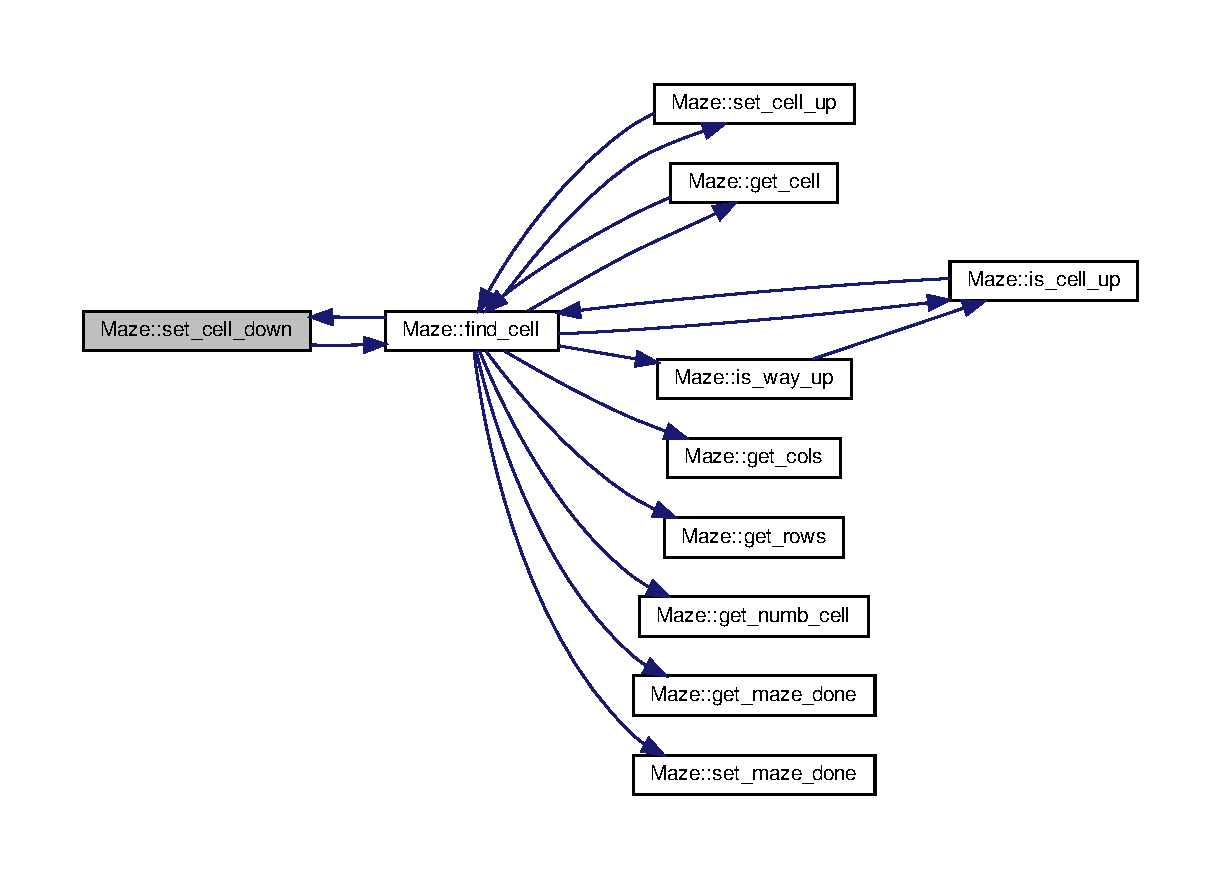
\includegraphics[width=350pt]{classMaze_ab86292a84aa56a26c4c07f4aa684d9bb_cgraph}
\end{center}
\end{figure}
Here is the caller graph for this function\+:\nopagebreak
\begin{figure}[H]
\begin{center}
\leavevmode
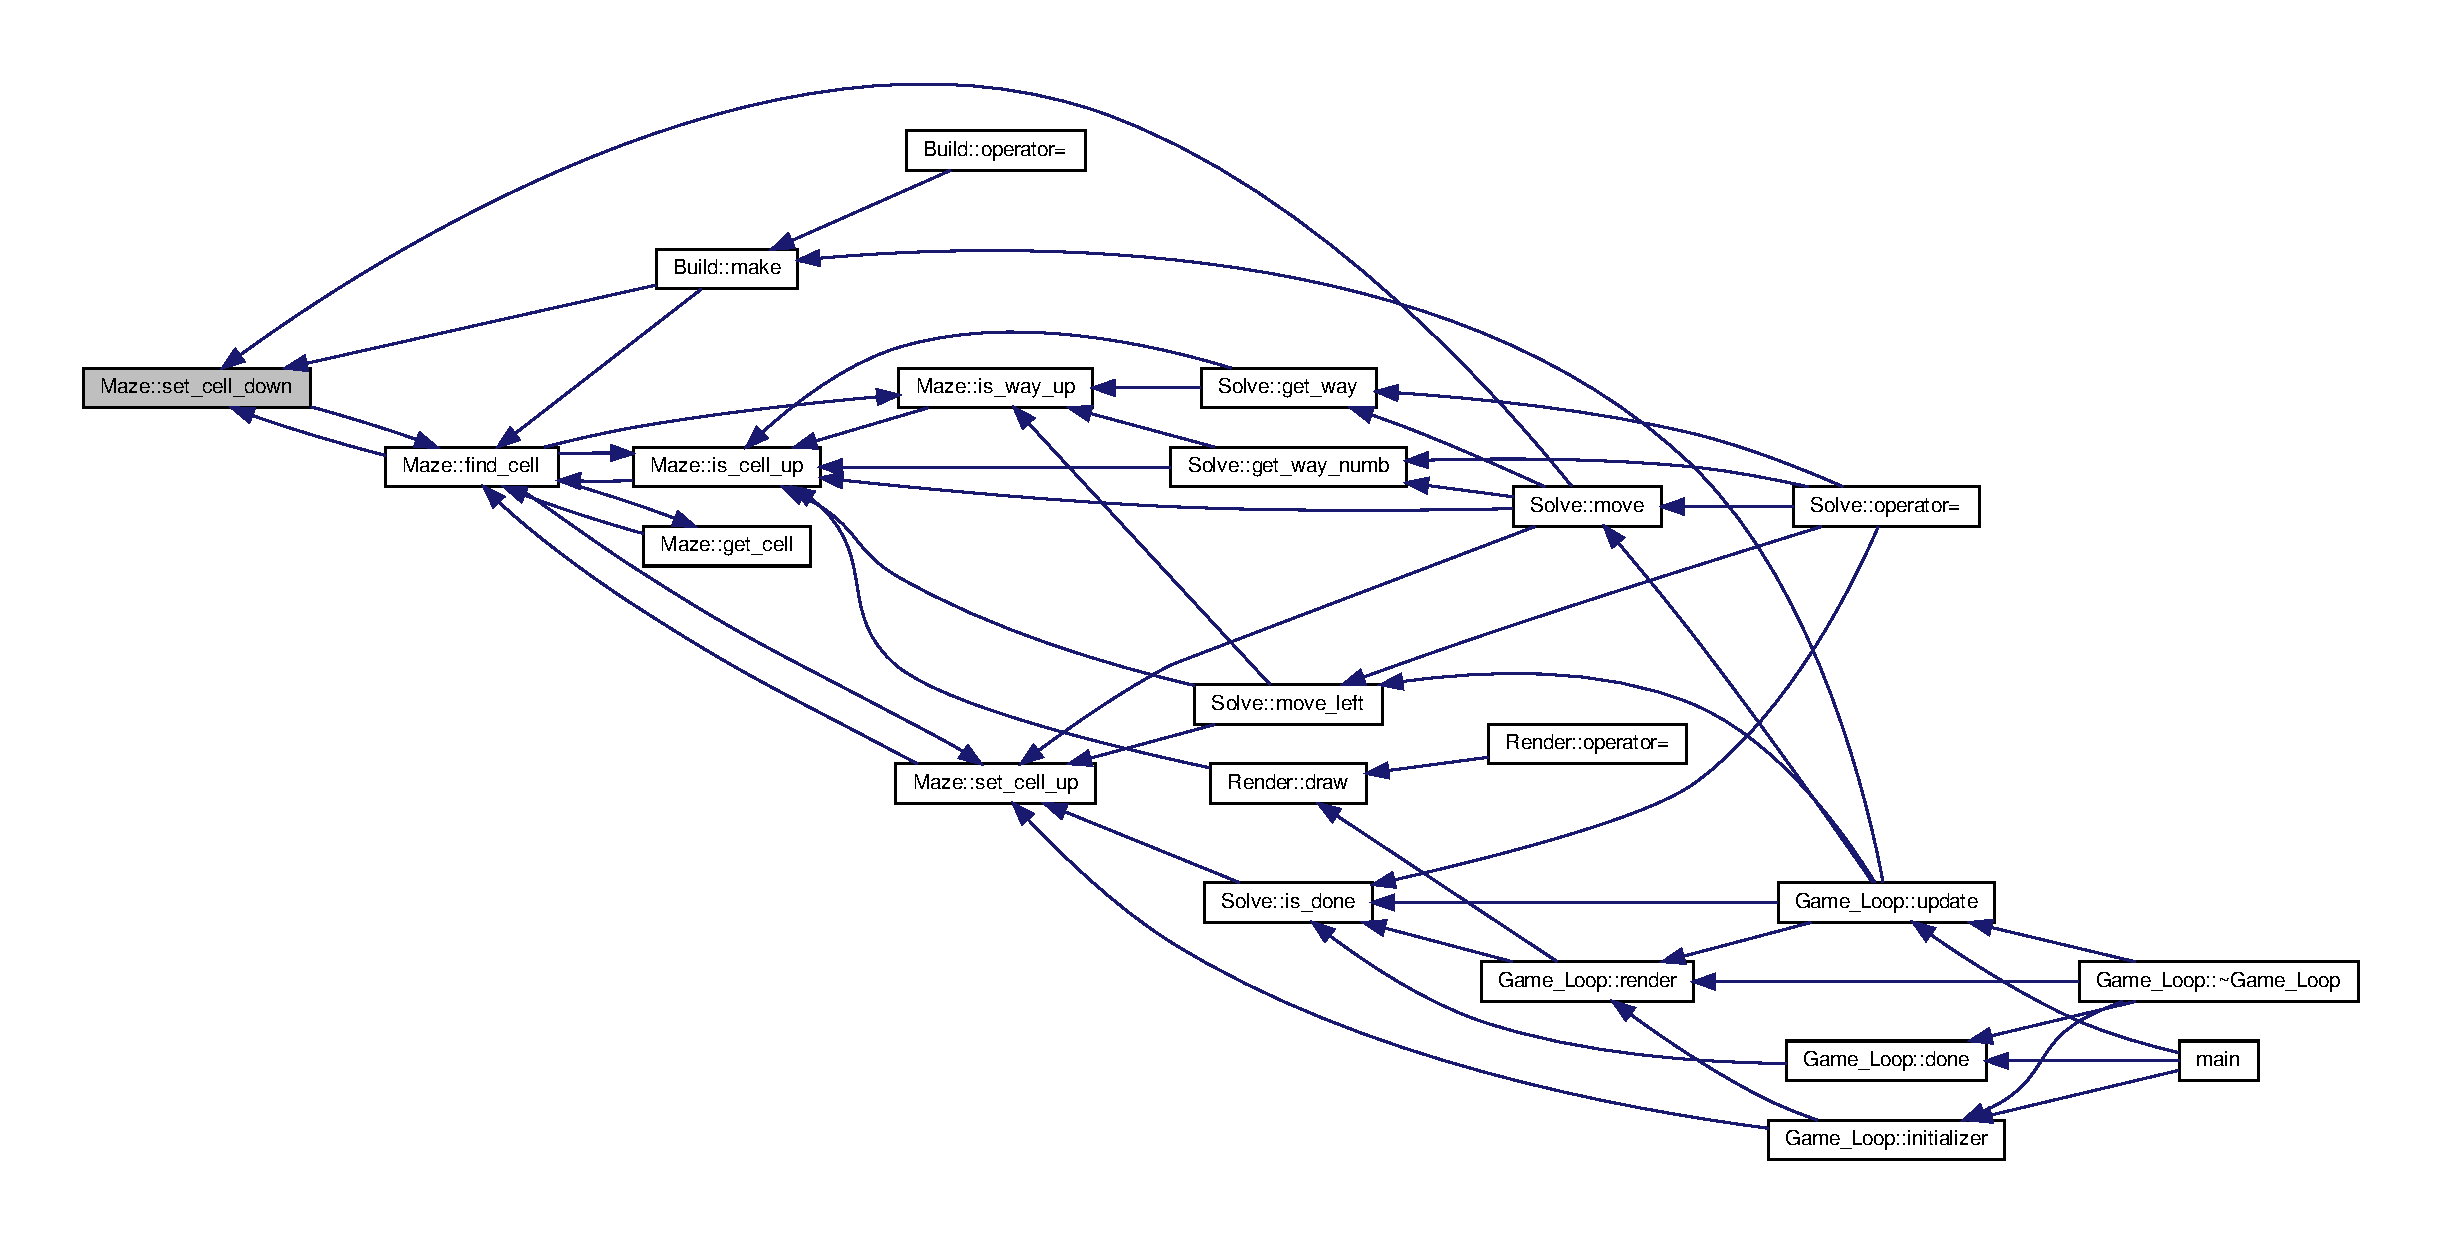
\includegraphics[width=350pt]{classMaze_ab86292a84aa56a26c4c07f4aa684d9bb_icgraph}
\end{center}
\end{figure}
\mbox{\Hypertarget{classMaze_a3635b71fab2c610376ae6613e7265fdf}\label{classMaze_a3635b71fab2c610376ae6613e7265fdf}} 
\index{Maze@{Maze}!set\+\_\+cell\+\_\+down@{set\+\_\+cell\+\_\+down}}
\index{set\+\_\+cell\+\_\+down@{set\+\_\+cell\+\_\+down}!Maze@{Maze}}
\subsubsection{\texorpdfstring{set\+\_\+cell\+\_\+down()}{set\_cell\_down()}\hspace{0.1cm}{\footnotesize\ttfamily [2/2]}}
{\footnotesize\ttfamily void Maze\+::set\+\_\+cell\+\_\+down (\begin{DoxyParamCaption}\item[{int}]{cell,  }\item[{\hyperlink{classMaze_a07167e321eac2b67100fb82ecb98f1d1}{status\+\_\+cell}}]{sc }\end{DoxyParamCaption})}



Method to change bit corresponding status cell to zero. 


\begin{DoxyParams}{Parameters}
{\em int} & cell of the vector. \\
\hline
{\em status\+\_\+cell} & sc status to be change. \\
\hline
\end{DoxyParams}

\begin{DoxyCode}
32 \{
33     m\_cell\_list[ cell] = ~m\_cell\_list [cell ] | (\hyperlink{maze_8h_a789d352559efaa396a258805d44f4289}{bit})sc;
34     m\_cell\_list[ cell ] = ~m\_cell\_list[ cell ];
35 \}
\end{DoxyCode}
\mbox{\Hypertarget{classMaze_aa7c832a91a3db8f48b31f688332f8986}\label{classMaze_aa7c832a91a3db8f48b31f688332f8986}} 
\index{Maze@{Maze}!set\+\_\+cell\+\_\+up@{set\+\_\+cell\+\_\+up}}
\index{set\+\_\+cell\+\_\+up@{set\+\_\+cell\+\_\+up}!Maze@{Maze}}
\subsubsection{\texorpdfstring{set\+\_\+cell\+\_\+up()}{set\_cell\_up()}\hspace{0.1cm}{\footnotesize\ttfamily [1/2]}}
{\footnotesize\ttfamily void Maze\+::set\+\_\+cell\+\_\+up (\begin{DoxyParamCaption}\item[{int}]{x,  }\item[{int}]{y,  }\item[{\hyperlink{classMaze_a07167e321eac2b67100fb82ecb98f1d1}{status\+\_\+cell}}]{sc }\end{DoxyParamCaption})}



Method to change bit corresponding status cell to one. 


\begin{DoxyParams}{Parameters}
{\em int} & x Coordinates X. \\
\hline
{\em int} & y Coordinates Y. \\
\hline
{\em status\+\_\+cell} & sc status to be change. \\
\hline
\end{DoxyParams}

\begin{DoxyCode}
15 \{
16     m\_cell\_list[ \hyperlink{classMaze_aa59b935dcd5f7129636cea6e40882c56}{find\_cell}(y,x) ] = m\_cell\_list[ \hyperlink{classMaze_aa59b935dcd5f7129636cea6e40882c56}{find\_cell}(y,x) ] | (
      \hyperlink{maze_8h_a789d352559efaa396a258805d44f4289}{bit})sc;
17 \}
\end{DoxyCode}
Here is the call graph for this function\+:\nopagebreak
\begin{figure}[H]
\begin{center}
\leavevmode
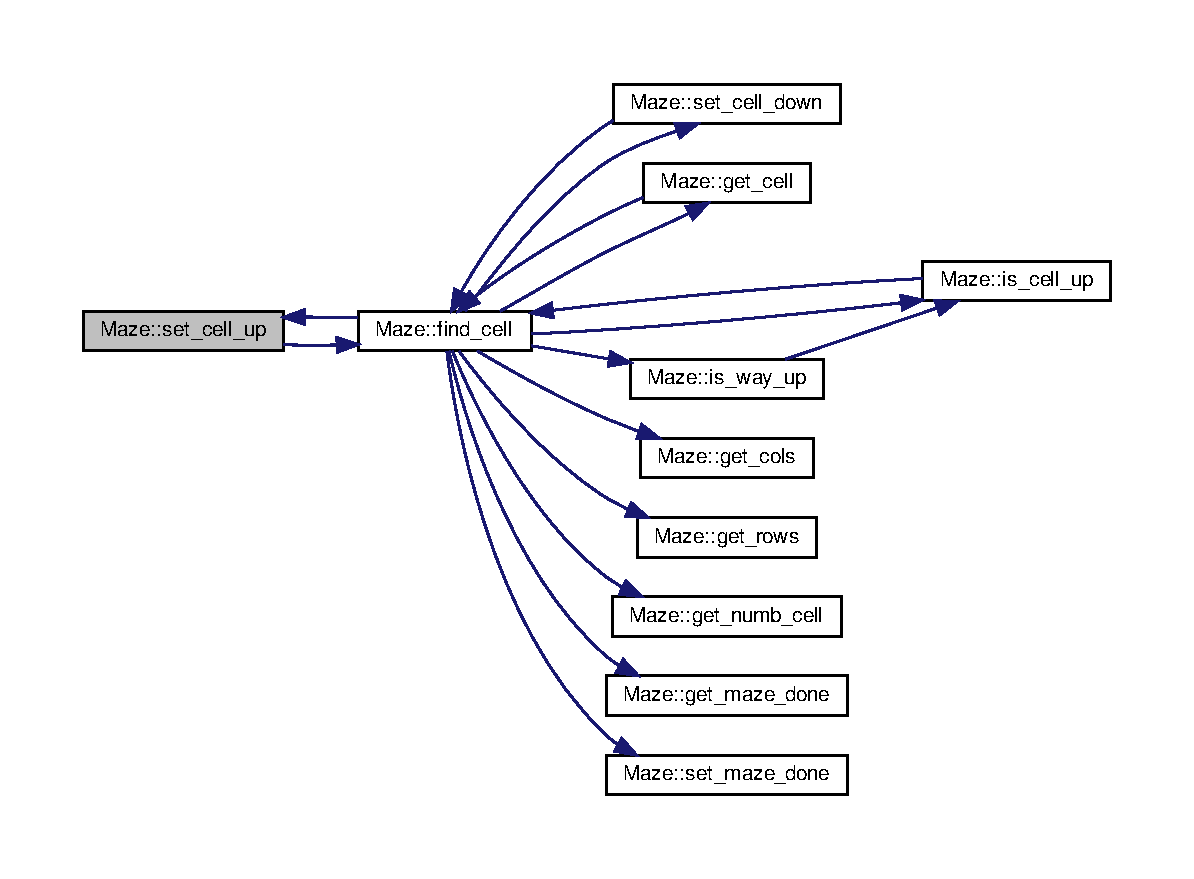
\includegraphics[width=350pt]{classMaze_aa7c832a91a3db8f48b31f688332f8986_cgraph}
\end{center}
\end{figure}
Here is the caller graph for this function\+:\nopagebreak
\begin{figure}[H]
\begin{center}
\leavevmode
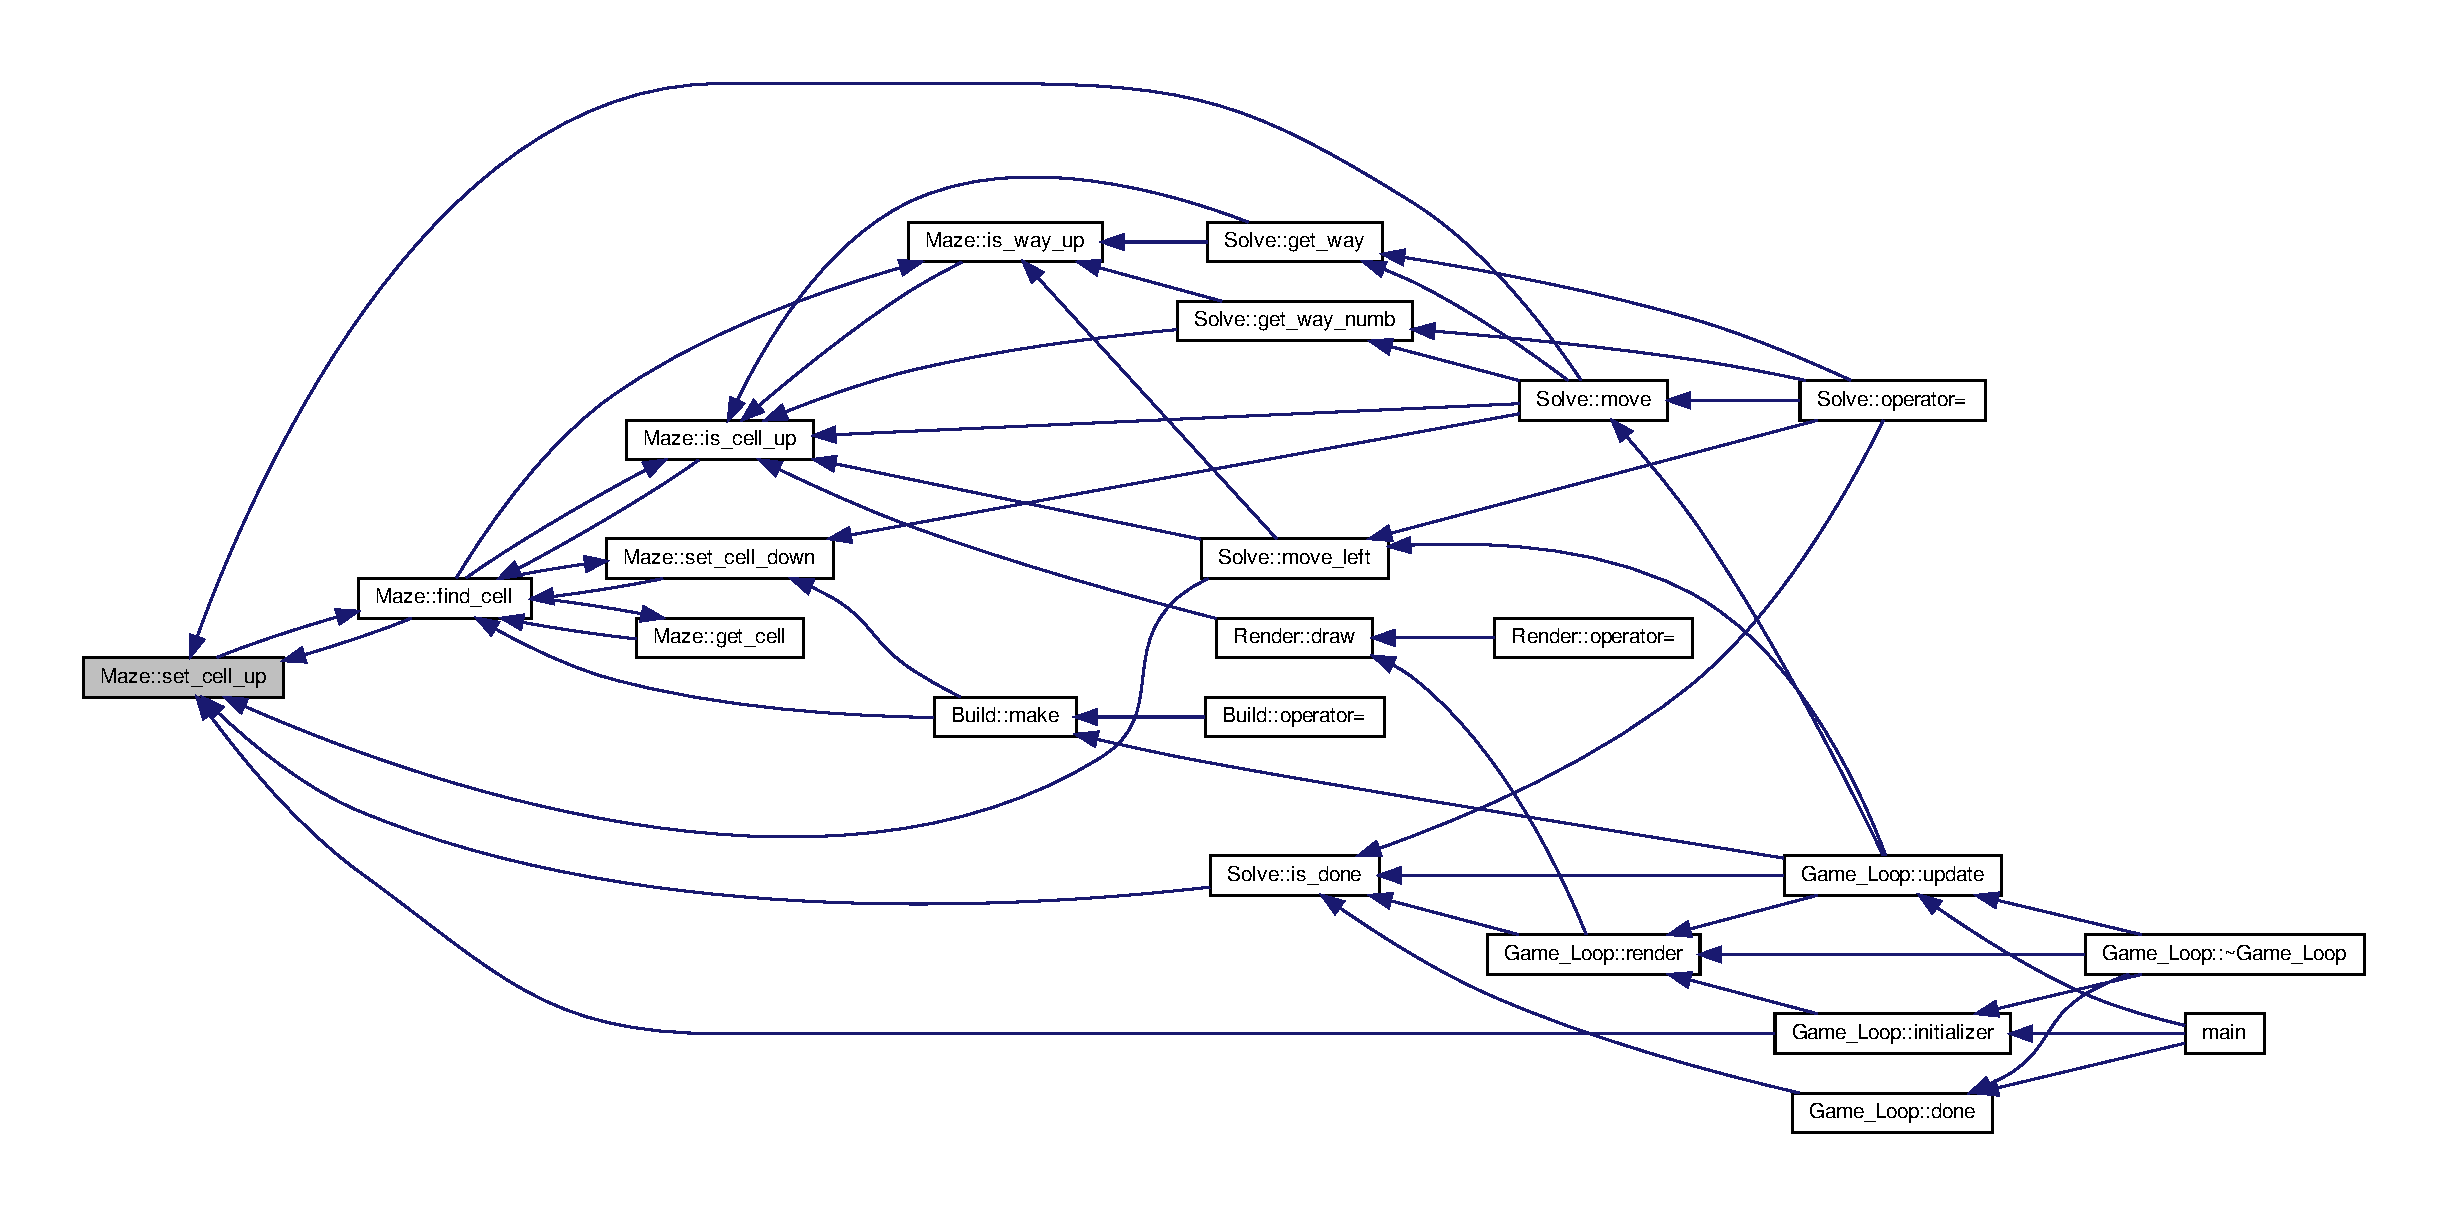
\includegraphics[width=350pt]{classMaze_aa7c832a91a3db8f48b31f688332f8986_icgraph}
\end{center}
\end{figure}
\mbox{\Hypertarget{classMaze_a53781b836de1a6b2c7ded74a2798b703}\label{classMaze_a53781b836de1a6b2c7ded74a2798b703}} 
\index{Maze@{Maze}!set\+\_\+cell\+\_\+up@{set\+\_\+cell\+\_\+up}}
\index{set\+\_\+cell\+\_\+up@{set\+\_\+cell\+\_\+up}!Maze@{Maze}}
\subsubsection{\texorpdfstring{set\+\_\+cell\+\_\+up()}{set\_cell\_up()}\hspace{0.1cm}{\footnotesize\ttfamily [2/2]}}
{\footnotesize\ttfamily void Maze\+::set\+\_\+cell\+\_\+up (\begin{DoxyParamCaption}\item[{int}]{cell,  }\item[{\hyperlink{classMaze_a07167e321eac2b67100fb82ecb98f1d1}{status\+\_\+cell}}]{sc }\end{DoxyParamCaption})}



Method to change bit corresponding status cell to one. 


\begin{DoxyParams}{Parameters}
{\em int} & cell of the vector. \\
\hline
{\em status\+\_\+cell} & sc status to be change. \\
\hline
\end{DoxyParams}

\begin{DoxyCode}
20 \{
21     m\_cell\_list[ cell ] = m\_cell\_list[ cell ] | (\hyperlink{maze_8h_a789d352559efaa396a258805d44f4289}{bit})sc;
22 
23 \}
\end{DoxyCode}
\mbox{\Hypertarget{classMaze_ab31ce10f6d3dfdd64d15c7b48f93ed63}\label{classMaze_ab31ce10f6d3dfdd64d15c7b48f93ed63}} 
\index{Maze@{Maze}!set\+\_\+maze\+\_\+done@{set\+\_\+maze\+\_\+done}}
\index{set\+\_\+maze\+\_\+done@{set\+\_\+maze\+\_\+done}!Maze@{Maze}}
\subsubsection{\texorpdfstring{set\+\_\+maze\+\_\+done()}{set\_maze\_done()}}
{\footnotesize\ttfamily void Maze\+::set\+\_\+maze\+\_\+done (\begin{DoxyParamCaption}\item[{int}]{x }\end{DoxyParamCaption})}


\begin{DoxyCode}
12 \{ m\_maze\_done = x; \}
\end{DoxyCode}
Here is the caller graph for this function\+:\nopagebreak
\begin{figure}[H]
\begin{center}
\leavevmode
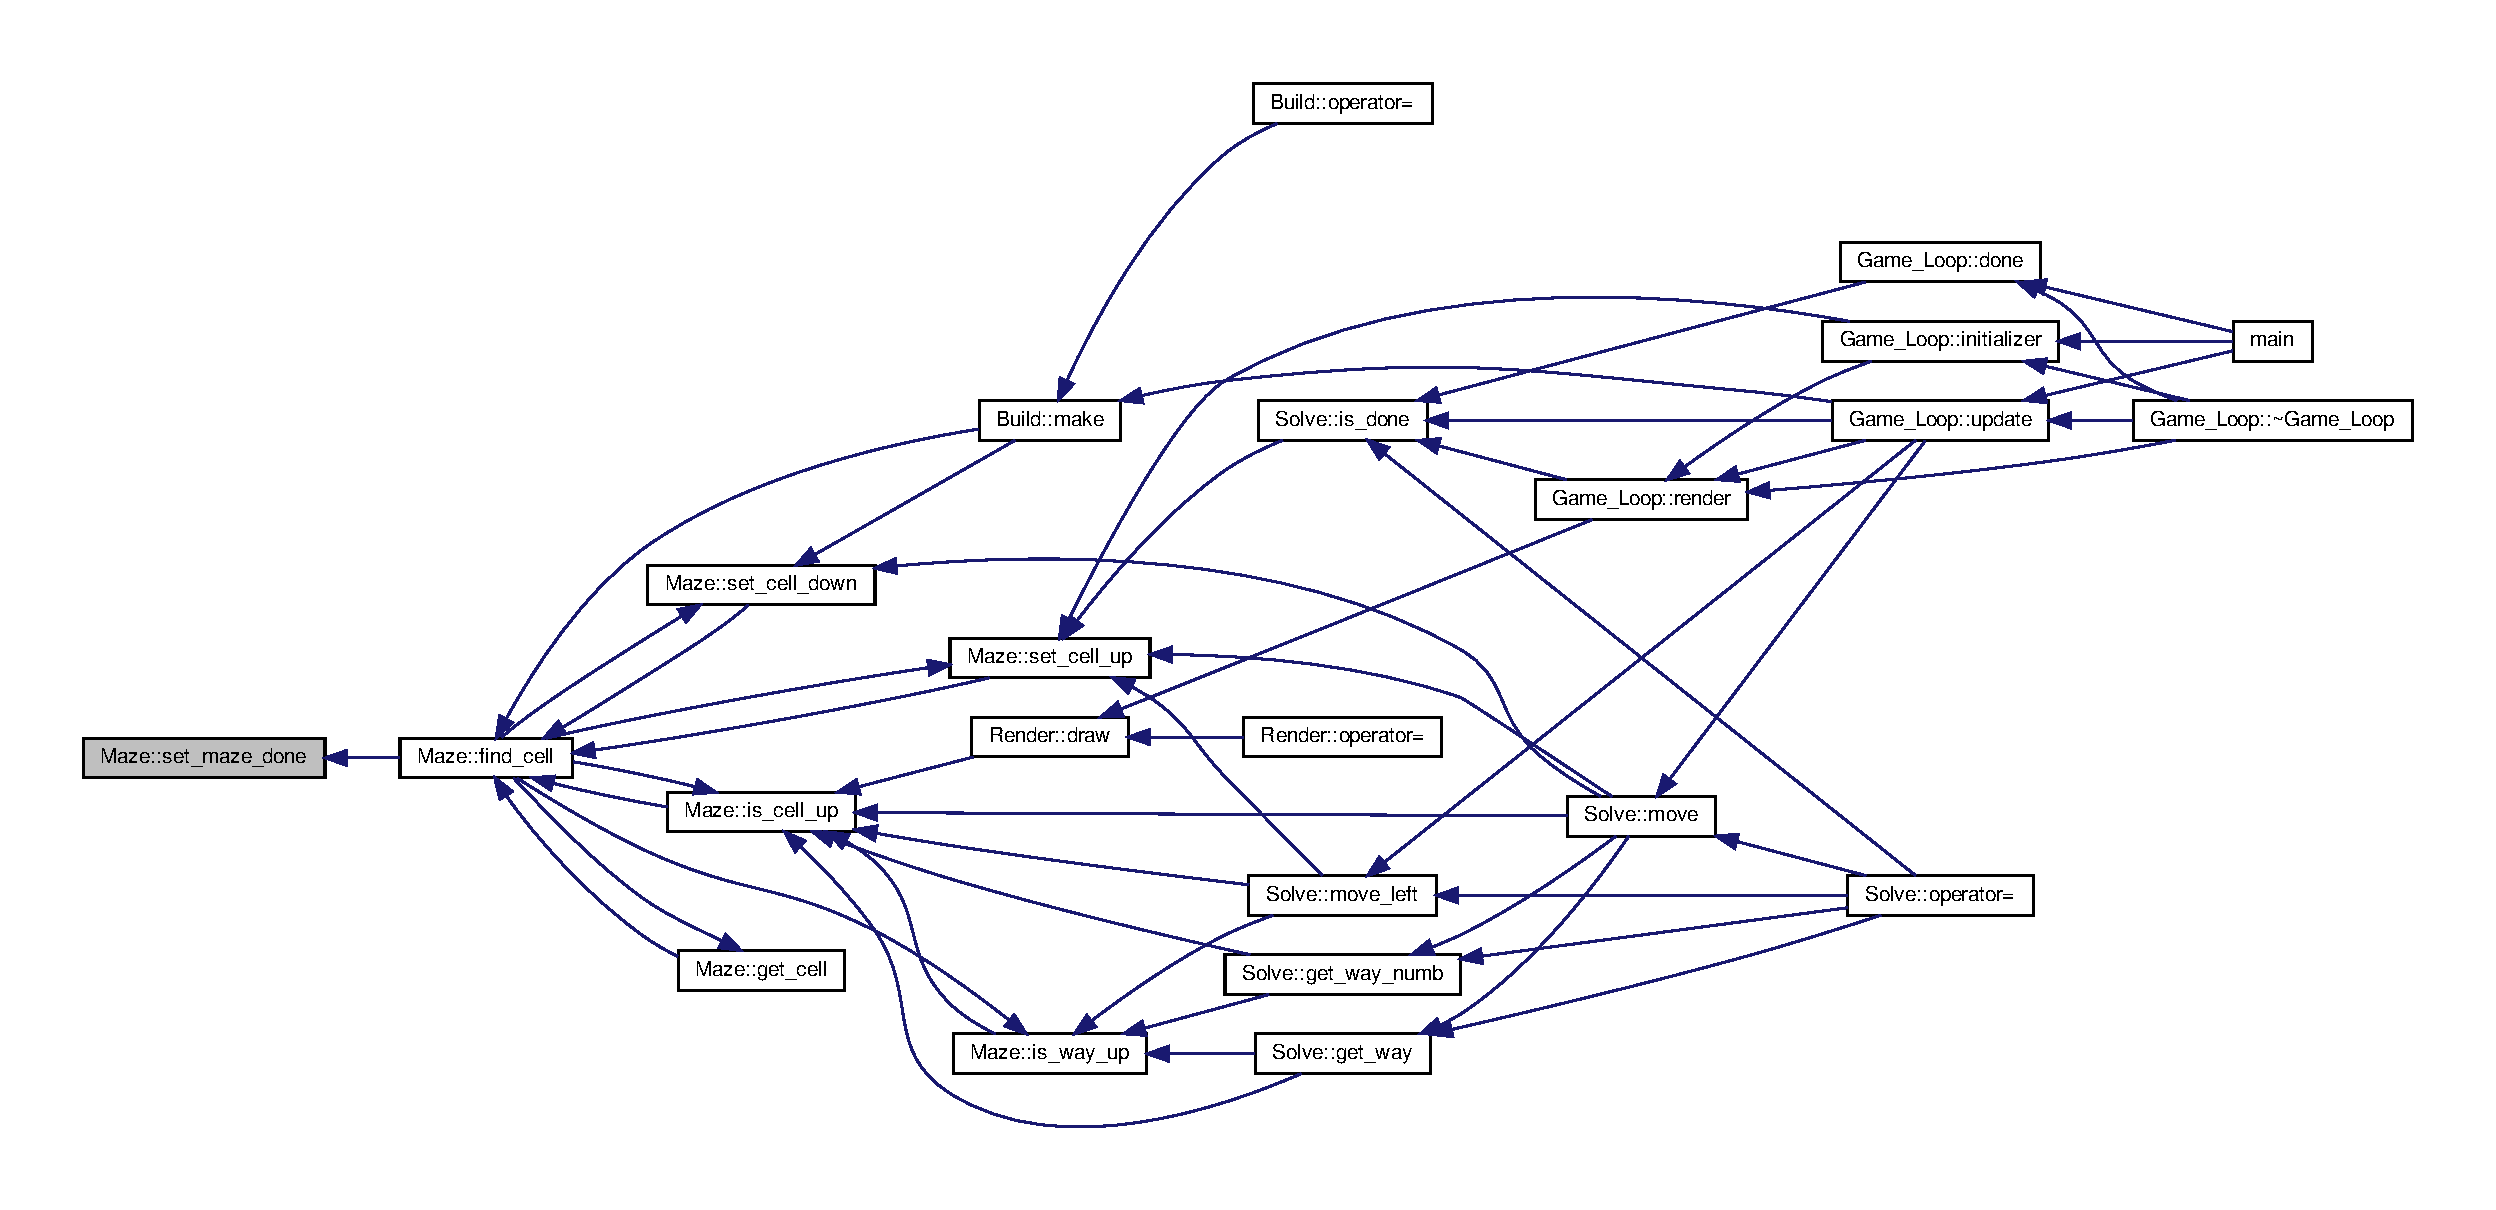
\includegraphics[width=350pt]{classMaze_ab31ce10f6d3dfdd64d15c7b48f93ed63_icgraph}
\end{center}
\end{figure}


The documentation for this class was generated from the following files\+:\begin{DoxyCompactItemize}
\item 
/home/bergony/lp\+\_\+magos/include/\hyperlink{maze_8h}{maze.\+h}\item 
/home/bergony/lp\+\_\+magos/src/\hyperlink{maze_8cpp}{maze.\+cpp}\end{DoxyCompactItemize}

\hypertarget{classRender}{}\section{Render Class Reference}
\label{classRender}\index{Render@{Render}}


{\bfseries Class} \hyperlink{classRender}{Render} {\itshape A class that recive \hyperlink{classMaze}{Maze} Object to draw in the \hyperlink{classCanvas}{Canvas}.}  




{\ttfamily \#include $<$render.\+h$>$}

\subsection*{Public Member Functions}
\begin{DoxyCompactItemize}
\item 
\hyperlink{classRender_a6e41bd186a63bf1852209ef34ea3d357}{Render} (\hyperlink{classMaze}{Maze} $\ast$m, int w=0, int h=0)
\begin{DoxyCompactList}\small\item\em ! Constructor \hyperlink{classRender}{Render} \end{DoxyCompactList}\item 
\hyperlink{classRender_ab0f4b917605cb15902f8d045a4197faf}{$\sim$\+Render} ()
\begin{DoxyCompactList}\small\item\em ! Destructors \hyperlink{classCanvas}{Canvas} \end{DoxyCompactList}\item 
\hyperlink{classRender_a034f7ab9a411cf3d6d379c27d4fe8115}{Render} (const \hyperlink{classRender}{Render} \&clone)
\begin{DoxyCompactList}\small\item\em ! Copy \hyperlink{classCanvas}{Canvas}. \end{DoxyCompactList}\item 
\hyperlink{classRender}{Render} \& \hyperlink{classRender_aeb62fc4c9d0a068daa1c848039bf7e6e}{operator=} (const \hyperlink{classRender}{Render} \&r)
\begin{DoxyCompactList}\small\item\em ! Assignment operator. \end{DoxyCompactList}\item 
void \hyperlink{classRender_a67e9fdbd6725960fd59d6350e8cd17cc}{draw} (std\+::string s)
\begin{DoxyCompactList}\small\item\em Method to draw the \hyperlink{classCanvas}{Canvas}. \end{DoxyCompactList}\end{DoxyCompactItemize}


\subsection{Detailed Description}
{\bfseries Class} \hyperlink{classRender}{Render} {\itshape A class that recive \hyperlink{classMaze}{Maze} Object to draw in the \hyperlink{classCanvas}{Canvas}.} 

\subsection{Constructor \& Destructor Documentation}
\mbox{\Hypertarget{classRender_a6e41bd186a63bf1852209ef34ea3d357}\label{classRender_a6e41bd186a63bf1852209ef34ea3d357}} 
\index{Render@{Render}!Render@{Render}}
\index{Render@{Render}!Render@{Render}}
\subsubsection{\texorpdfstring{Render()}{Render()}\hspace{0.1cm}{\footnotesize\ttfamily [1/2]}}
{\footnotesize\ttfamily Render\+::\+Render (\begin{DoxyParamCaption}\item[{\hyperlink{classMaze}{Maze} $\ast$}]{m,  }\item[{int}]{w = {\ttfamily 0},  }\item[{int}]{h = {\ttfamily 0} }\end{DoxyParamCaption})\hspace{0.3cm}{\ttfamily [inline]}}



! Constructor \hyperlink{classRender}{Render} 


\begin{DoxyParams}{Parameters}
{\em int} & $\ast$M Reference to \hyperlink{classMaze}{Maze}. \\
\hline
{\em int} & w width of Image. \\
\hline
{\em int} & h height of Image. \\
\hline
\end{DoxyParams}

\begin{DoxyCode}
27                                                 : m\_maze\{m\}, m\_cell\_width\{w\}, m\_cell\_height\{h\}, m\_canvas\{ w
       , h \}
28         \{
29             m\_cell\_width = (w-40) / m\_maze->\hyperlink{classMaze_a8a04cd1335e96a80358181afa164d4c9}{get\_cols}();
30             m\_cell\_height = (h-40) / m\_maze->\hyperlink{classMaze_ac786606a34632b2254b2d27d5f5f0f3f}{get\_rows}();
31         \}
\end{DoxyCode}
Here is the call graph for this function\+:\nopagebreak
\begin{figure}[H]
\begin{center}
\leavevmode
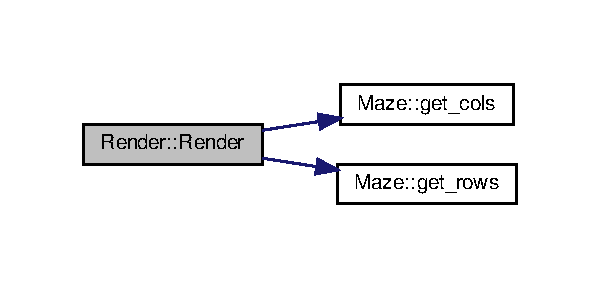
\includegraphics[width=288pt]{classRender_a6e41bd186a63bf1852209ef34ea3d357_cgraph}
\end{center}
\end{figure}
\mbox{\Hypertarget{classRender_ab0f4b917605cb15902f8d045a4197faf}\label{classRender_ab0f4b917605cb15902f8d045a4197faf}} 
\index{Render@{Render}!````~Render@{$\sim$\+Render}}
\index{````~Render@{$\sim$\+Render}!Render@{Render}}
\subsubsection{\texorpdfstring{$\sim$\+Render()}{~Render()}}
{\footnotesize\ttfamily Render\+::$\sim$\+Render (\begin{DoxyParamCaption}{ }\end{DoxyParamCaption})\hspace{0.3cm}{\ttfamily [inline]}}



! Destructors \hyperlink{classCanvas}{Canvas} 


\begin{DoxyCode}
34 \{ \textcolor{comment}{/* EMPTY */} \}
\end{DoxyCode}
\mbox{\Hypertarget{classRender_a034f7ab9a411cf3d6d379c27d4fe8115}\label{classRender_a034f7ab9a411cf3d6d379c27d4fe8115}} 
\index{Render@{Render}!Render@{Render}}
\index{Render@{Render}!Render@{Render}}
\subsubsection{\texorpdfstring{Render()}{Render()}\hspace{0.1cm}{\footnotesize\ttfamily [2/2]}}
{\footnotesize\ttfamily Render\+::\+Render (\begin{DoxyParamCaption}\item[{const \hyperlink{classRender}{Render} \&}]{clone }\end{DoxyParamCaption})\hspace{0.3cm}{\ttfamily [inline]}}



! Copy \hyperlink{classCanvas}{Canvas}. 


\begin{DoxyCode}
38         \{
39             m\_maze = clone.m\_maze;
40             m\_cell\_width = clone.m\_cell\_width;
41             m\_cell\_height = clone.m\_cell\_width;
42             m\_canvas = clone.m\_canvas;
43         \}
\end{DoxyCode}


\subsection{Member Function Documentation}
\mbox{\Hypertarget{classRender_a67e9fdbd6725960fd59d6350e8cd17cc}\label{classRender_a67e9fdbd6725960fd59d6350e8cd17cc}} 
\index{Render@{Render}!draw@{draw}}
\index{draw@{draw}!Render@{Render}}
\subsubsection{\texorpdfstring{draw()}{draw()}}
{\footnotesize\ttfamily void Render\+::draw (\begin{DoxyParamCaption}\item[{std\+::string}]{s }\end{DoxyParamCaption})}



Method to draw the \hyperlink{classCanvas}{Canvas}. 


\begin{DoxyParams}{Parameters}
{\em std\+::string} & s name of string output. \\
\hline
\end{DoxyParams}

\begin{DoxyCode}
15 \{
16     m\_canvas.\hyperlink{classCanvas_a0205269b201aed71f21b8f613cd66333}{clear}( \hyperlink{render_8cpp_a009fdb656a368e46b7d614e7438b5830}{GRAY} );     \textcolor{comment}{// Clear the canvas.}
17 
18     \textcolor{keyword}{const} \textcolor{keywordtype}{char} *word = &s.at(0); \textcolor{comment}{// point begin of word}
19 
20     \textcolor{keywordtype}{int} off\_set\_width = m\_cell\_width - ( m\_cell\_width * 95 ) / 100;      \textcolor{comment}{//Distance of lines}
21     \textcolor{keywordtype}{int} off\_set\_height = m\_cell\_height - ( m\_cell\_height * 95 ) / 100;   \textcolor{comment}{//Distance of lines}
22 
23     \textcolor{keywordflow}{for}(\textcolor{keywordtype}{int} i\{0\}, y\{0\}; i < ( m\_maze->\hyperlink{classMaze_ac786606a34632b2254b2d27d5f5f0f3f}{get\_rows}() * m\_cell\_height ); y++, i += m\_cell\_height )
24     \{
25         \textcolor{keywordflow}{for}(\textcolor{keywordtype}{int} j\{0\}, x\{0\}; j < ( m\_maze->\hyperlink{classMaze_a8a04cd1335e96a80358181afa164d4c9}{get\_cols}() * m\_cell\_width );x++, j += m\_cell\_width )
26         \{
27             \textcolor{comment}{//Draw top line.}
28             \textcolor{keywordflow}{if}(y == 0 || ( m\_maze->\hyperlink{classMaze_a2b0e69e72d6c3e1037578f057946a21e}{is\_cell\_up}(y , x, 
      \hyperlink{classMaze_a07167e321eac2b67100fb82ecb98f1d1ab28354b543375bfa94dabaeda722927f}{Maze::status\_cell::top}) && m\_maze->\hyperlink{classMaze_a2b0e69e72d6c3e1037578f057946a21e}{is\_cell\_up}(y-1,x,
      \hyperlink{classMaze_a07167e321eac2b67100fb82ecb98f1d1a74e8333ad11685ff3bdae589c8f6e34d}{Maze::status\_cell::down}) ) )
29             \{
30                 m\_canvas.\hyperlink{classCanvas_a3095d5ff2670c5dc9939454198865ceb}{hline}( 20+j , 20+i , m\_cell\_width, \hyperlink{render_8cpp_ada1558ae37a1ddfc6c8b784f809385d4}{BLACK});
31             \}
32 
33             \textcolor{comment}{//Draw Left line.}
34             \textcolor{keywordflow}{if}(x == 0 || ( m\_maze->\hyperlink{classMaze_a2b0e69e72d6c3e1037578f057946a21e}{is\_cell\_up}(y, x, 
      \hyperlink{classMaze_a07167e321eac2b67100fb82ecb98f1d1a811882fecd5c7618d7099ebbd39ea254}{Maze::status\_cell::left}) && m\_maze->\hyperlink{classMaze_a2b0e69e72d6c3e1037578f057946a21e}{is\_cell\_up}(y,x-1,
      \hyperlink{classMaze_a07167e321eac2b67100fb82ecb98f1d1a7c4f29407893c334a6cb7a87bf045c0d}{Maze::status\_cell::right}) ) )
35             \{
36                 m\_canvas.\hyperlink{classCanvas_af81ae19142bc132665e053ce5de15211}{vline}(20+j , 20+i , m\_cell\_height, \hyperlink{render_8cpp_ada1558ae37a1ddfc6c8b784f809385d4}{BLACK});
37             \}
38 
39             \textcolor{comment}{//Draw a yellow box if is way.}
40             \textcolor{keywordflow}{if}( m\_maze->\hyperlink{classMaze_a2b0e69e72d6c3e1037578f057946a21e}{is\_cell\_up}(y , x, \hyperlink{classMaze_a07167e321eac2b67100fb82ecb98f1d1ac83b72dd001482ce10f0b106c7a0ed0e}{Maze::status\_cell::way}) )
41             \{
42                 m\_canvas.\hyperlink{classCanvas_a6e1c6baa6fb92cd3de1726b67b51aa38}{box}(off\_set\_width+j, off\_set\_height+i, m\_cell\_height-(off\_set\_height*2), 
      m\_cell\_width-(off\_set\_width*2), \hyperlink{render_8cpp_a0616d169807ac93a808a3928d058d2d5}{YELLOW});         
43             \}
44 
45             \textcolor{comment}{//Draw a red box if is discarde.}
46             \textcolor{keywordflow}{if}( m\_maze->\hyperlink{classMaze_a2b0e69e72d6c3e1037578f057946a21e}{is\_cell\_up}(y , x, \hyperlink{classMaze_a07167e321eac2b67100fb82ecb98f1d1a94708897ec9db8647dfe695714c98e46}{Maze::status\_cell::discarded}
      ) )
47             \{
48                 m\_canvas.\hyperlink{classCanvas_a6e1c6baa6fb92cd3de1726b67b51aa38}{box}(off\_set\_width+j, off\_set\_height+i, m\_cell\_height-(off\_set\_height*2), 
      m\_cell\_width-(off\_set\_width*2), \hyperlink{render_8cpp_a0db58550f21b0b45458ade7d071c3500}{RED});         
49             \}
50 
51             \textcolor{comment}{//Draw the way to Top if true.}
52             \textcolor{keywordflow}{if}( m\_maze->\hyperlink{classMaze_a2b0e69e72d6c3e1037578f057946a21e}{is\_cell\_up}(y , x, \hyperlink{classMaze_a07167e321eac2b67100fb82ecb98f1d1ac83b72dd001482ce10f0b106c7a0ed0e}{Maze::status\_cell::way}) &&  
      m\_maze->\hyperlink{classMaze_a2b0e69e72d6c3e1037578f057946a21e}{is\_cell\_up}(y-1 , x, \hyperlink{classMaze_a07167e321eac2b67100fb82ecb98f1d1ac83b72dd001482ce10f0b106c7a0ed0e}{Maze::status\_cell::way}) && !m\_maze->
      \hyperlink{classMaze_a2b0e69e72d6c3e1037578f057946a21e}{is\_cell\_up}( y, x,\hyperlink{classMaze_a07167e321eac2b67100fb82ecb98f1d1ab28354b543375bfa94dabaeda722927f}{Maze::status\_cell::top} ) )
53             \{
54                 m\_canvas.\hyperlink{classCanvas_a6e1c6baa6fb92cd3de1726b67b51aa38}{box}(off\_set\_width+j, i, m\_cell\_height-(off\_set\_height*2), m\_cell\_width-(
      off\_set\_width*2), \hyperlink{render_8cpp_a0616d169807ac93a808a3928d058d2d5}{YELLOW});         
55             \}
56             \textcolor{comment}{//Draw the way to Left is true.}
57             \textcolor{keywordflow}{if}( m\_maze->\hyperlink{classMaze_a2b0e69e72d6c3e1037578f057946a21e}{is\_cell\_up}(y , x, \hyperlink{classMaze_a07167e321eac2b67100fb82ecb98f1d1ac83b72dd001482ce10f0b106c7a0ed0e}{Maze::status\_cell::way}) &&  
      m\_maze->\hyperlink{classMaze_a2b0e69e72d6c3e1037578f057946a21e}{is\_cell\_up}(y , x-1, \hyperlink{classMaze_a07167e321eac2b67100fb82ecb98f1d1ac83b72dd001482ce10f0b106c7a0ed0e}{Maze::status\_cell::way}) && !m\_maze->
      \hyperlink{classMaze_a2b0e69e72d6c3e1037578f057946a21e}{is\_cell\_up}( y, x,\hyperlink{classMaze_a07167e321eac2b67100fb82ecb98f1d1a811882fecd5c7618d7099ebbd39ea254}{Maze::status\_cell::left}))
58             \{
59                 m\_canvas.\hyperlink{classCanvas_a6e1c6baa6fb92cd3de1726b67b51aa38}{box}(j, off\_set\_height+i, m\_cell\_height-(off\_set\_height*2), m\_cell\_width-(
      off\_set\_width*2), \hyperlink{render_8cpp_a0616d169807ac93a808a3928d058d2d5}{YELLOW});
60             \}
61             \textcolor{comment}{//Draw the way to Down if true.}
62             \textcolor{keywordflow}{if}( m\_maze->\hyperlink{classMaze_a2b0e69e72d6c3e1037578f057946a21e}{is\_cell\_up}(y , x, \hyperlink{classMaze_a07167e321eac2b67100fb82ecb98f1d1ac83b72dd001482ce10f0b106c7a0ed0e}{Maze::status\_cell::way}) &&  
      m\_maze->\hyperlink{classMaze_a2b0e69e72d6c3e1037578f057946a21e}{is\_cell\_up}(y+1 , x, \hyperlink{classMaze_a07167e321eac2b67100fb82ecb98f1d1ac83b72dd001482ce10f0b106c7a0ed0e}{Maze::status\_cell::way}) && !m\_maze->
      \hyperlink{classMaze_a2b0e69e72d6c3e1037578f057946a21e}{is\_cell\_up}( y, x,\hyperlink{classMaze_a07167e321eac2b67100fb82ecb98f1d1a74e8333ad11685ff3bdae589c8f6e34d}{Maze::status\_cell::down}))
63             \{
64                 m\_canvas.\hyperlink{classCanvas_a6e1c6baa6fb92cd3de1726b67b51aa38}{box}(off\_set\_width+j, off\_set\_height+i, m\_cell\_height, m\_cell\_width-(
      off\_set\_width*2), \hyperlink{render_8cpp_a0616d169807ac93a808a3928d058d2d5}{YELLOW});         
65             \}
66             \textcolor{comment}{//Draw the way to right if true.}
67             \textcolor{keywordflow}{if}( m\_maze->\hyperlink{classMaze_a2b0e69e72d6c3e1037578f057946a21e}{is\_cell\_up}(y , x, \hyperlink{classMaze_a07167e321eac2b67100fb82ecb98f1d1ac83b72dd001482ce10f0b106c7a0ed0e}{Maze::status\_cell::way}) &&  
      m\_maze->\hyperlink{classMaze_a2b0e69e72d6c3e1037578f057946a21e}{is\_cell\_up}(y , x+1, \hyperlink{classMaze_a07167e321eac2b67100fb82ecb98f1d1ac83b72dd001482ce10f0b106c7a0ed0e}{Maze::status\_cell::way}) && !m\_maze->
      \hyperlink{classMaze_a2b0e69e72d6c3e1037578f057946a21e}{is\_cell\_up}( y, x,\hyperlink{classMaze_a07167e321eac2b67100fb82ecb98f1d1a7c4f29407893c334a6cb7a87bf045c0d}{Maze::status\_cell::right}))
68             \{
69                 m\_canvas.\hyperlink{classCanvas_a6e1c6baa6fb92cd3de1726b67b51aa38}{box}(off\_set\_width+j, off\_set\_height+i, m\_cell\_height-(off\_set\_height*2), 
      m\_cell\_width, \hyperlink{render_8cpp_a0616d169807ac93a808a3928d058d2d5}{YELLOW});         
70             \}
71             \textcolor{comment}{//Draw the Discarde to top if true.}
72             \textcolor{keywordflow}{if}( m\_maze->\hyperlink{classMaze_a2b0e69e72d6c3e1037578f057946a21e}{is\_cell\_up}(y , x, \hyperlink{classMaze_a07167e321eac2b67100fb82ecb98f1d1a94708897ec9db8647dfe695714c98e46}{Maze::status\_cell::discarded}
      ) &&  m\_maze->\hyperlink{classMaze_a2b0e69e72d6c3e1037578f057946a21e}{is\_cell\_up}(y-1 , x, \hyperlink{classMaze_a07167e321eac2b67100fb82ecb98f1d1a94708897ec9db8647dfe695714c98e46}{Maze::status\_cell::discarded}) && !
      m\_maze->\hyperlink{classMaze_a2b0e69e72d6c3e1037578f057946a21e}{is\_cell\_up}( y, x,\hyperlink{classMaze_a07167e321eac2b67100fb82ecb98f1d1ab28354b543375bfa94dabaeda722927f}{Maze::status\_cell::top}))
73             \{
74                 m\_canvas.\hyperlink{classCanvas_a6e1c6baa6fb92cd3de1726b67b51aa38}{box}(off\_set\_width+j, i, m\_cell\_height-(off\_set\_height*2), m\_cell\_width-(
      off\_set\_width*2), \hyperlink{render_8cpp_a0db58550f21b0b45458ade7d071c3500}{RED});         
75             \}
76             \textcolor{comment}{//Draw the Discarde to left if true.}
77             \textcolor{keywordflow}{if}( m\_maze->\hyperlink{classMaze_a2b0e69e72d6c3e1037578f057946a21e}{is\_cell\_up}(y , x, \hyperlink{classMaze_a07167e321eac2b67100fb82ecb98f1d1a94708897ec9db8647dfe695714c98e46}{Maze::status\_cell::discarded}
      ) &&  m\_maze->\hyperlink{classMaze_a2b0e69e72d6c3e1037578f057946a21e}{is\_cell\_up}(y , x-1, \hyperlink{classMaze_a07167e321eac2b67100fb82ecb98f1d1a94708897ec9db8647dfe695714c98e46}{Maze::status\_cell::discarded}) && !
      m\_maze->\hyperlink{classMaze_a2b0e69e72d6c3e1037578f057946a21e}{is\_cell\_up}( y, x,\hyperlink{classMaze_a07167e321eac2b67100fb82ecb98f1d1a811882fecd5c7618d7099ebbd39ea254}{Maze::status\_cell::left}))
78             \{
79                 m\_canvas.\hyperlink{classCanvas_a6e1c6baa6fb92cd3de1726b67b51aa38}{box}(j, off\_set\_height+i, m\_cell\_height-(off\_set\_height*2), m\_cell\_width-(
      off\_set\_width*2), \hyperlink{render_8cpp_a0db58550f21b0b45458ade7d071c3500}{RED});         
80             \}
81             \textcolor{comment}{//Draw the Discarde to down if true.}
82             \textcolor{keywordflow}{if}( m\_maze->\hyperlink{classMaze_a2b0e69e72d6c3e1037578f057946a21e}{is\_cell\_up}(y , x, \hyperlink{classMaze_a07167e321eac2b67100fb82ecb98f1d1a94708897ec9db8647dfe695714c98e46}{Maze::status\_cell::discarded}
      ) &&  m\_maze->\hyperlink{classMaze_a2b0e69e72d6c3e1037578f057946a21e}{is\_cell\_up}(y+1 , x, \hyperlink{classMaze_a07167e321eac2b67100fb82ecb98f1d1a94708897ec9db8647dfe695714c98e46}{Maze::status\_cell::discarded}) && !
      m\_maze->\hyperlink{classMaze_a2b0e69e72d6c3e1037578f057946a21e}{is\_cell\_up}( y, x,\hyperlink{classMaze_a07167e321eac2b67100fb82ecb98f1d1a74e8333ad11685ff3bdae589c8f6e34d}{Maze::status\_cell::down}))
83             \{
84                 m\_canvas.\hyperlink{classCanvas_a6e1c6baa6fb92cd3de1726b67b51aa38}{box}(off\_set\_width+j, off\_set\_height+i, m\_cell\_height, m\_cell\_width-(
      off\_set\_width*2), \hyperlink{render_8cpp_a0db58550f21b0b45458ade7d071c3500}{RED});         
85             \}
86             \textcolor{comment}{//Draw the Discarde to right if true.}
87             \textcolor{keywordflow}{if}( m\_maze->\hyperlink{classMaze_a2b0e69e72d6c3e1037578f057946a21e}{is\_cell\_up}(y , x, \hyperlink{classMaze_a07167e321eac2b67100fb82ecb98f1d1a94708897ec9db8647dfe695714c98e46}{Maze::status\_cell::discarded}
      ) &&  m\_maze->\hyperlink{classMaze_a2b0e69e72d6c3e1037578f057946a21e}{is\_cell\_up}(y , x+1, \hyperlink{classMaze_a07167e321eac2b67100fb82ecb98f1d1a94708897ec9db8647dfe695714c98e46}{Maze::status\_cell::discarded}) && !
      m\_maze->\hyperlink{classMaze_a2b0e69e72d6c3e1037578f057946a21e}{is\_cell\_up}( y, x,\hyperlink{classMaze_a07167e321eac2b67100fb82ecb98f1d1a7c4f29407893c334a6cb7a87bf045c0d}{Maze::status\_cell::right}))
88             \{
89                 m\_canvas.\hyperlink{classCanvas_a6e1c6baa6fb92cd3de1726b67b51aa38}{box}(off\_set\_width+j, off\_set\_height+i, m\_cell\_height-(off\_set\_height*2), 
      m\_cell\_width, \hyperlink{render_8cpp_a0db58550f21b0b45458ade7d071c3500}{RED});         
90             \}
91             \textcolor{comment}{//Draw the exit box Green.}
92             \textcolor{keywordflow}{if}( m\_maze->\hyperlink{classMaze_a2b0e69e72d6c3e1037578f057946a21e}{is\_cell\_up}(y , x, \hyperlink{classMaze_a07167e321eac2b67100fb82ecb98f1d1af24f62eeb789199b9b2e467df3b1876b}{Maze::status\_cell::exit}) )
93             \{
94                 m\_canvas.\hyperlink{classCanvas_a6e1c6baa6fb92cd3de1726b67b51aa38}{box}((off\_set\_width*2)+j, (off\_set\_height*2)+i, m\_cell\_height-(off\_set\_height*4)
      , m\_cell\_width-(off\_set\_width*4), \hyperlink{render_8cpp_a58d827358f6165cc5927d28b2dcff311}{GREEN});         
95             \}
96             \textcolor{comment}{//Draw the Entrace Box Blue.}
97             \textcolor{keywordflow}{if}( m\_maze->\hyperlink{classMaze_a2b0e69e72d6c3e1037578f057946a21e}{is\_cell\_up}(y , x, \hyperlink{classMaze_a07167e321eac2b67100fb82ecb98f1d1a31f57c97180bdc320a97370c71cf524a}{Maze::status\_cell::entrace}) )
98             \{
99                 m\_canvas.\hyperlink{classCanvas_a6e1c6baa6fb92cd3de1726b67b51aa38}{box}((off\_set\_width*2)+j, (off\_set\_height*2)+i, m\_cell\_height-(off\_set\_height*4)
      , m\_cell\_width-(off\_set\_width*4), \hyperlink{render_8cpp_ab49b84fe87ce8b46e7e4a25be82c7538}{BLUE});         
100             \}
101         \}
102         \textcolor{comment}{//Draw Right Line.}
103         m\_canvas.\hyperlink{classCanvas_af81ae19142bc132665e053ce5de15211}{vline}(20+(m\_cell\_width * m\_maze->\hyperlink{classMaze_a8a04cd1335e96a80358181afa164d4c9}{get\_cols}()), 20+i , m\_cell\_height , 
      \hyperlink{render_8cpp_ada1558ae37a1ddfc6c8b784f809385d4}{BLACK});
104     \}
105     \textcolor{comment}{//Draw Down line.}
106     m\_canvas.\hyperlink{classCanvas_a3095d5ff2670c5dc9939454198865ceb}{hline}(20, 20+(m\_cell\_height*m\_maze->\hyperlink{classMaze_ac786606a34632b2254b2d27d5f5f0f3f}{get\_rows}() ), m\_cell\_width * m\_maze->
      \hyperlink{classMaze_a8a04cd1335e96a80358181afa164d4c9}{get\_cols}() + 1, \hyperlink{render_8cpp_ada1558ae37a1ddfc6c8b784f809385d4}{BLACK});
107 
108     stbi\_write\_png\_compression\_level = 0;    \textcolor{comment}{// defaults to 8; set to higher for more compression}
109     stbi\_write\_png( word,            \textcolor{comment}{// file name}
110             m\_canvas.\hyperlink{classCanvas_a8478392f133ddaf1c9b7272a301c7898}{get\_w}(), m\_canvas.\hyperlink{classCanvas_ab26c7ab91a0a9069895285a314bc8418}{get\_h}(),           \textcolor{comment}{// image dimensions}
111             3,                              \textcolor{comment}{// # of channels per pixel}
112             m\_canvas.\hyperlink{classCanvas_aa9f9b173d57058ea827a0134c937d0e1}{get\_p}(),                      \textcolor{comment}{// the pixels}
113             m\_canvas.\hyperlink{classCanvas_a8478392f133ddaf1c9b7272a301c7898}{get\_w}()* 3);                 \textcolor{comment}{// length of a row (in bytes), see above.}
114 
115 \}
\end{DoxyCode}
Here is the call graph for this function\+:\nopagebreak
\begin{figure}[H]
\begin{center}
\leavevmode
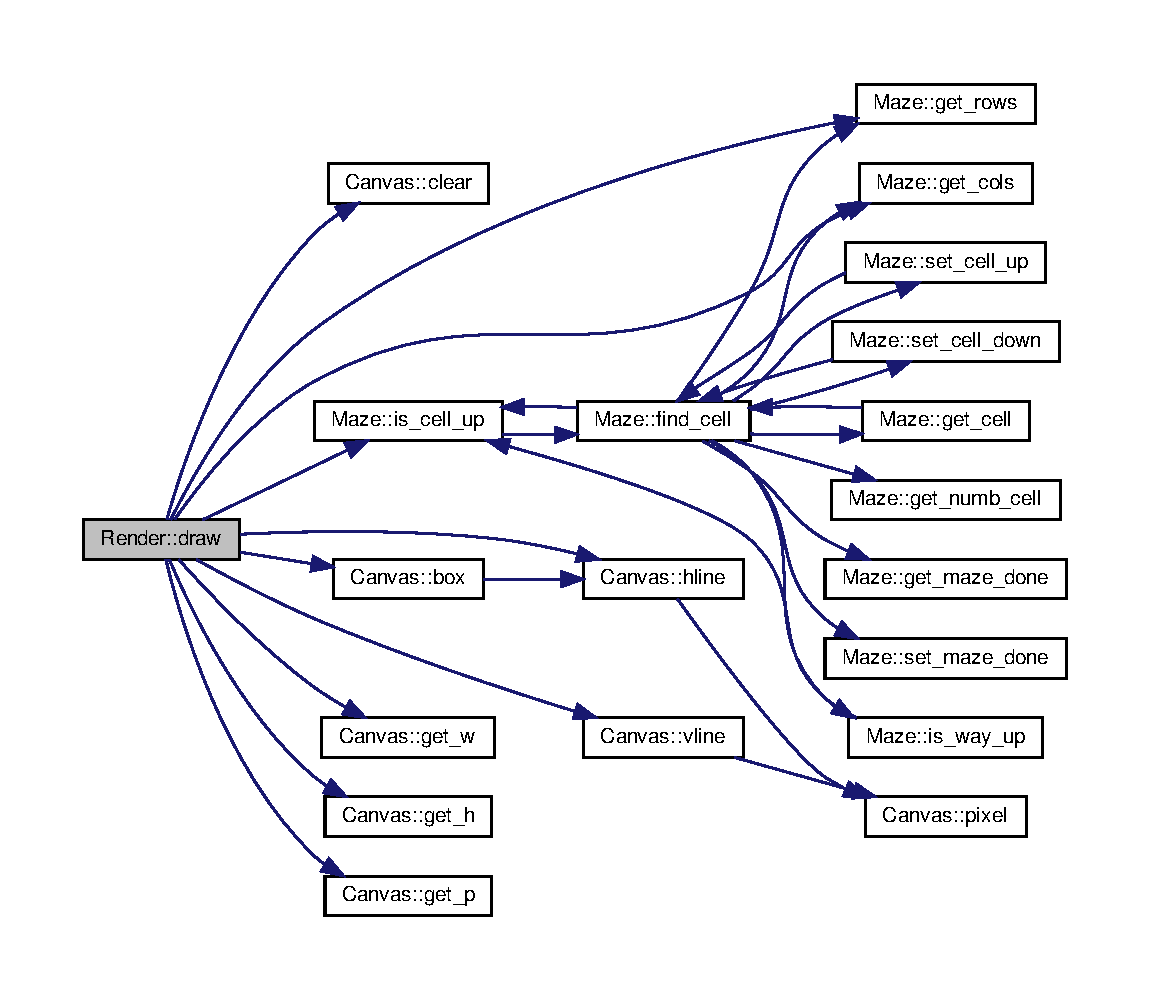
\includegraphics[width=350pt]{classRender_a67e9fdbd6725960fd59d6350e8cd17cc_cgraph}
\end{center}
\end{figure}
Here is the caller graph for this function\+:\nopagebreak
\begin{figure}[H]
\begin{center}
\leavevmode
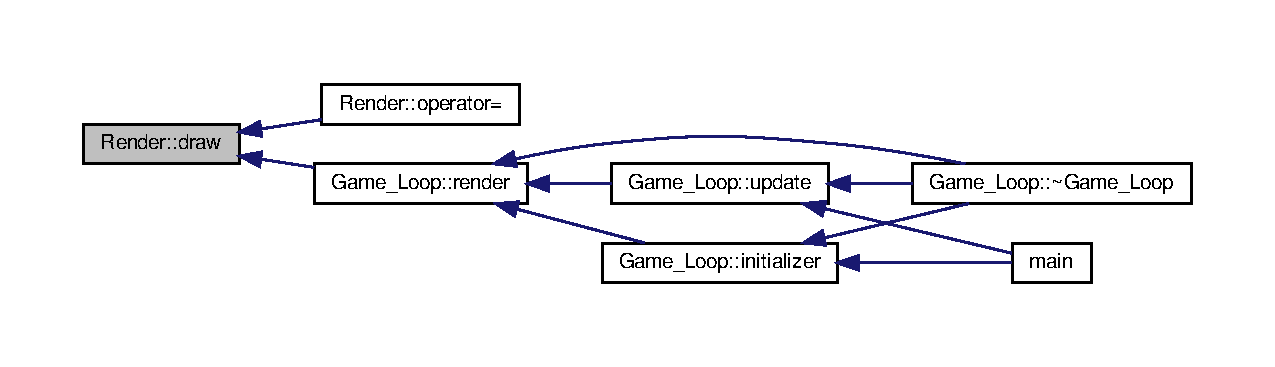
\includegraphics[width=350pt]{classRender_a67e9fdbd6725960fd59d6350e8cd17cc_icgraph}
\end{center}
\end{figure}
\mbox{\Hypertarget{classRender_aeb62fc4c9d0a068daa1c848039bf7e6e}\label{classRender_aeb62fc4c9d0a068daa1c848039bf7e6e}} 
\index{Render@{Render}!operator=@{operator=}}
\index{operator=@{operator=}!Render@{Render}}
\subsubsection{\texorpdfstring{operator=()}{operator=()}}
{\footnotesize\ttfamily \hyperlink{classRender}{Render}\& Render\+::operator= (\begin{DoxyParamCaption}\item[{const \hyperlink{classRender}{Render} \&}]{r }\end{DoxyParamCaption})\hspace{0.3cm}{\ttfamily [inline]}}



! Assignment operator. 


\begin{DoxyCode}
47         \{
48             this->m\_maze = r.m\_maze;
49             this->m\_cell\_width = r.m\_cell\_width;
50             this->m\_cell\_height = r.m\_cell\_width;
51             this->m\_canvas = r.m\_canvas;
52 
53             \textcolor{keywordflow}{return} *\textcolor{keyword}{this};
54         \}
\end{DoxyCode}
Here is the call graph for this function\+:\nopagebreak
\begin{figure}[H]
\begin{center}
\leavevmode
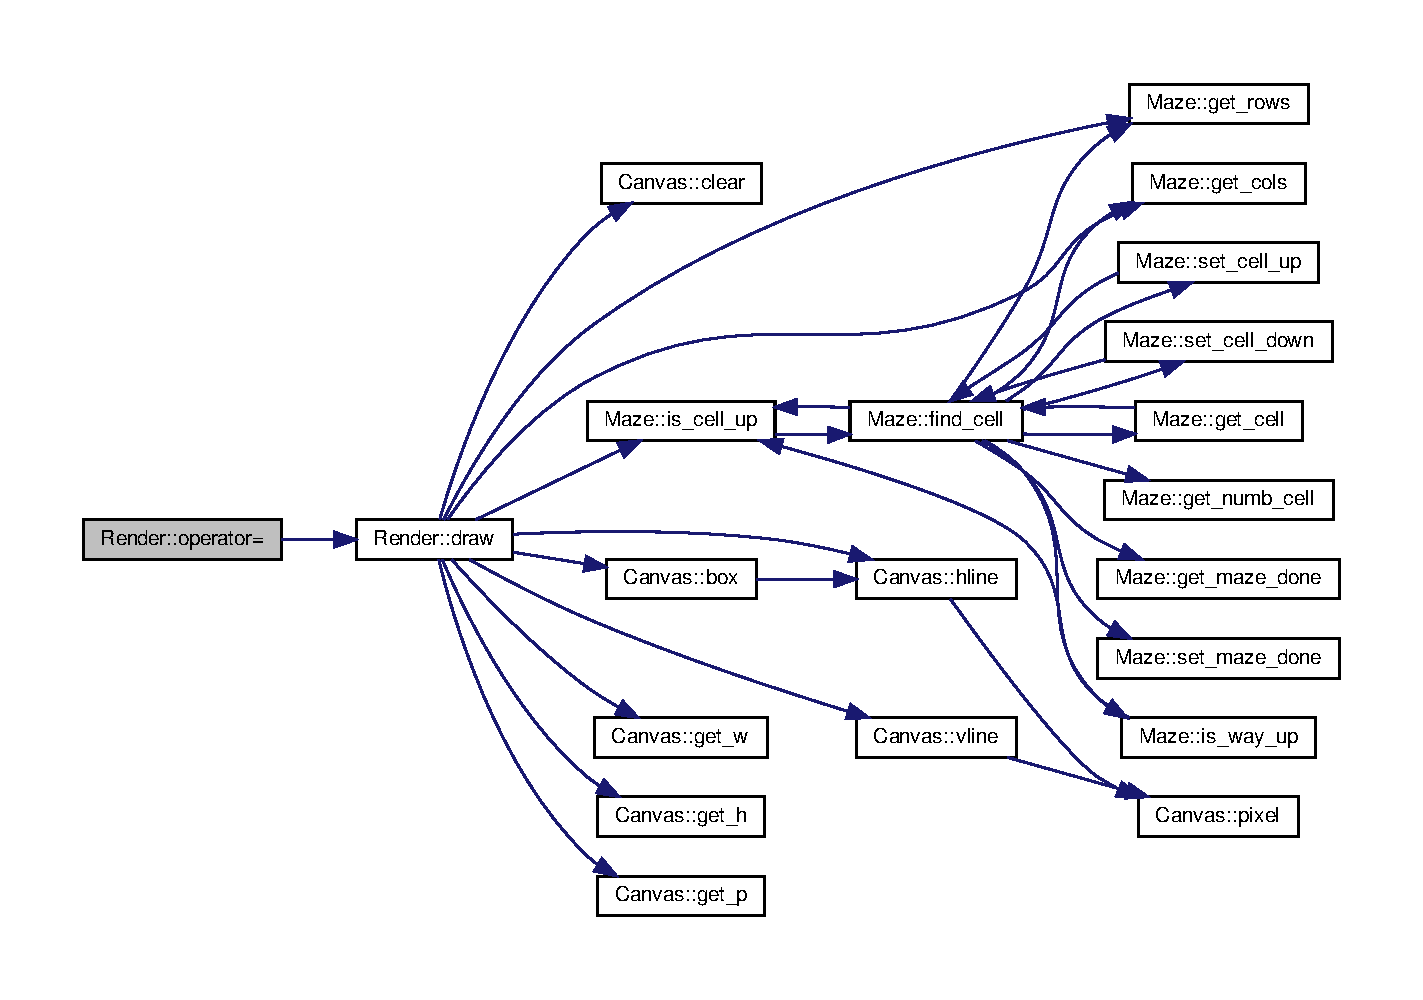
\includegraphics[width=350pt]{classRender_aeb62fc4c9d0a068daa1c848039bf7e6e_cgraph}
\end{center}
\end{figure}


The documentation for this class was generated from the following files\+:\begin{DoxyCompactItemize}
\item 
/home/bergony/lp\+\_\+magos/include/\hyperlink{render_8h}{render.\+h}\item 
/home/bergony/lp\+\_\+magos/src/\hyperlink{render_8cpp}{render.\+cpp}\end{DoxyCompactItemize}

\hypertarget{classSolve}{}\section{Solve Class Reference}
\label{classSolve}\index{Solve@{Solve}}


{\bfseries Class} \hyperlink{classSolve}{Solve} {\itshape Class that recive a \hyperlink{classMaze}{Maze} to be \hyperlink{classSolve}{Solve}.}  




{\ttfamily \#include $<$solve.\+h$>$}

\subsection*{Public Member Functions}
\begin{DoxyCompactItemize}
\item 
\hyperlink{classSolve_a3aeaf8dfa8f2bb5f8fb4ec048b9afdb9}{Solve} (\hyperlink{classMaze}{Maze} $\ast$m)
\begin{DoxyCompactList}\small\item\em ! Constructor \hyperlink{classSolve}{Solve} \end{DoxyCompactList}\item 
\hyperlink{classSolve_ac437f1307c9d4669205ac7d370a55ffc}{Solve} ()
\begin{DoxyCompactList}\small\item\em ! Constructor \hyperlink{classSolve}{Solve} Default \end{DoxyCompactList}\item 
\hyperlink{classSolve_a3435d6ff721c2d8bebf0eff2411fa93e}{$\sim$\+Solve} (void)
\begin{DoxyCompactList}\small\item\em ! Destructors \hyperlink{classSolve}{Solve} \end{DoxyCompactList}\item 
\hyperlink{classSolve_ac78c2c56eb847decb6efd070978a9a3d}{Solve} (const \hyperlink{classSolve}{Solve} \&clone)
\begin{DoxyCompactList}\small\item\em ! Copy \hyperlink{classSolve}{Solve} \end{DoxyCompactList}\item 
\hyperlink{classSolve}{Solve} \& \hyperlink{classSolve_a2c0330bee4d1cafc5b3c7d5f7ba72697}{operator=} (const \hyperlink{classSolve}{Solve} \&s)
\begin{DoxyCompactList}\small\item\em ! Assignment operator. \end{DoxyCompactList}\item 
bool \hyperlink{classSolve_a868db181d288fdb10e5592b62e669c3b}{is\+\_\+done} (void)
\begin{DoxyCompactList}\small\item\em ! Method to check if the maze is Done \end{DoxyCompactList}\item 
void \hyperlink{classSolve_a963b593c0311f03c7e4ce77eea818fa1}{get\+\_\+way} (void)
\begin{DoxyCompactList}\small\item\em ! Method to get with way de player\+\_\+cell goes save on way stack \end{DoxyCompactList}\item 
int \hyperlink{classSolve_aaccff68d3e175f7400a9407077db7255}{get\+\_\+way\+\_\+numb} (void)
\begin{DoxyCompactList}\small\item\em ! Method to get numbers of posible ways \end{DoxyCompactList}\item 
void \hyperlink{classSolve_a8902b46862c7759928495e3684054f82}{move} (void)
\begin{DoxyCompactList}\small\item\em ! Move to the next Cell backtrack. \end{DoxyCompactList}\item 
bool \hyperlink{classSolve_a8226032eb1d4877539f417d4fab0efde}{move\+\_\+left} (void)
\begin{DoxyCompactList}\small\item\em ! Move to the next cell left hand. \end{DoxyCompactList}\end{DoxyCompactItemize}


\subsection{Detailed Description}
{\bfseries Class} \hyperlink{classSolve}{Solve} {\itshape Class that recive a \hyperlink{classMaze}{Maze} to be \hyperlink{classSolve}{Solve}.} 

\subsection{Constructor \& Destructor Documentation}
\mbox{\Hypertarget{classSolve_a3aeaf8dfa8f2bb5f8fb4ec048b9afdb9}\label{classSolve_a3aeaf8dfa8f2bb5f8fb4ec048b9afdb9}} 
\index{Solve@{Solve}!Solve@{Solve}}
\index{Solve@{Solve}!Solve@{Solve}}
\subsubsection{\texorpdfstring{Solve()}{Solve()}\hspace{0.1cm}{\footnotesize\ttfamily [1/3]}}
{\footnotesize\ttfamily Solve\+::\+Solve (\begin{DoxyParamCaption}\item[{\hyperlink{classMaze}{Maze} $\ast$}]{m }\end{DoxyParamCaption})\hspace{0.3cm}{\ttfamily [inline]}}



! Constructor \hyperlink{classSolve}{Solve} 


\begin{DoxyParams}{Parameters}
{\em \hyperlink{classMaze}{Maze}} & $\ast$m Reference to a maze. \\
\hline
\end{DoxyParams}

\begin{DoxyCode}
33                        : m\_maze\{m\} 
34         \{
35             \textcolor{comment}{/* EMPTY */}
36         \}
\end{DoxyCode}
\mbox{\Hypertarget{classSolve_ac437f1307c9d4669205ac7d370a55ffc}\label{classSolve_ac437f1307c9d4669205ac7d370a55ffc}} 
\index{Solve@{Solve}!Solve@{Solve}}
\index{Solve@{Solve}!Solve@{Solve}}
\subsubsection{\texorpdfstring{Solve()}{Solve()}\hspace{0.1cm}{\footnotesize\ttfamily [2/3]}}
{\footnotesize\ttfamily Solve\+::\+Solve (\begin{DoxyParamCaption}{ }\end{DoxyParamCaption})\hspace{0.3cm}{\ttfamily [inline]}}



! Constructor \hyperlink{classSolve}{Solve} Default 


\begin{DoxyCode}
39 \{\}
\end{DoxyCode}
\mbox{\Hypertarget{classSolve_a3435d6ff721c2d8bebf0eff2411fa93e}\label{classSolve_a3435d6ff721c2d8bebf0eff2411fa93e}} 
\index{Solve@{Solve}!````~Solve@{$\sim$\+Solve}}
\index{````~Solve@{$\sim$\+Solve}!Solve@{Solve}}
\subsubsection{\texorpdfstring{$\sim$\+Solve()}{~Solve()}}
{\footnotesize\ttfamily Solve\+::$\sim$\+Solve (\begin{DoxyParamCaption}\item[{void}]{ }\end{DoxyParamCaption})\hspace{0.3cm}{\ttfamily [inline]}}



! Destructors \hyperlink{classSolve}{Solve} 


\begin{DoxyCode}
42 \{ \}
\end{DoxyCode}
\mbox{\Hypertarget{classSolve_ac78c2c56eb847decb6efd070978a9a3d}\label{classSolve_ac78c2c56eb847decb6efd070978a9a3d}} 
\index{Solve@{Solve}!Solve@{Solve}}
\index{Solve@{Solve}!Solve@{Solve}}
\subsubsection{\texorpdfstring{Solve()}{Solve()}\hspace{0.1cm}{\footnotesize\ttfamily [3/3]}}
{\footnotesize\ttfamily Solve\+::\+Solve (\begin{DoxyParamCaption}\item[{const \hyperlink{classSolve}{Solve} \&}]{clone }\end{DoxyParamCaption})\hspace{0.3cm}{\ttfamily [inline]}}



! Copy \hyperlink{classSolve}{Solve} 


\begin{DoxyCode}
46         \{   
47             m\_maze = clone.m\_maze;
48             m\_stack\_cell = clone.m\_stack\_cell;
49             m\_stack\_ways = clone.m\_stack\_ways;
50             m\_cell\_player = clone.m\_cell\_player;
51             m\_numb\_way = clone.m\_numb\_way;
52         \}
\end{DoxyCode}


\subsection{Member Function Documentation}
\mbox{\Hypertarget{classSolve_a963b593c0311f03c7e4ce77eea818fa1}\label{classSolve_a963b593c0311f03c7e4ce77eea818fa1}} 
\index{Solve@{Solve}!get\+\_\+way@{get\+\_\+way}}
\index{get\+\_\+way@{get\+\_\+way}!Solve@{Solve}}
\subsubsection{\texorpdfstring{get\+\_\+way()}{get\_way()}}
{\footnotesize\ttfamily void Solve\+::get\+\_\+way (\begin{DoxyParamCaption}\item[{void}]{ }\end{DoxyParamCaption})}



! Method to get with way de player\+\_\+cell goes save on way stack 


\begin{DoxyCode}
16 \{
17     \textcolor{keywordflow}{if}( !m\_maze->\hyperlink{classMaze_a2b0e69e72d6c3e1037578f057946a21e}{is\_cell\_up}( m\_cell\_player, \hyperlink{classMaze_a07167e321eac2b67100fb82ecb98f1d1ab28354b543375bfa94dabaeda722927f}{Maze::status\_cell::top}) &&
18             !m\_maze->\hyperlink{classMaze_a308fa695665de6217c0e7f28aab5adda}{is\_way\_up}( m\_cell\_player -  m\_maze->\hyperlink{classMaze_a8a04cd1335e96a80358181afa164d4c9}{get\_cols}() ))
19     \{
20         m\_stack\_ways.push(1);
21     \}
22     \textcolor{keywordflow}{if}( !m\_maze->\hyperlink{classMaze_a2b0e69e72d6c3e1037578f057946a21e}{is\_cell\_up}( m\_cell\_player, \hyperlink{classMaze_a07167e321eac2b67100fb82ecb98f1d1a811882fecd5c7618d7099ebbd39ea254}{Maze::status\_cell::left}) &&
23             !m\_maze->\hyperlink{classMaze_a308fa695665de6217c0e7f28aab5adda}{is\_way\_up}( m\_cell\_player-1 ))
24     \{
25         m\_stack\_ways.push(2);
26     \}
27     \textcolor{keywordflow}{if}( !m\_maze->\hyperlink{classMaze_a2b0e69e72d6c3e1037578f057946a21e}{is\_cell\_up}( m\_cell\_player, \hyperlink{classMaze_a07167e321eac2b67100fb82ecb98f1d1a74e8333ad11685ff3bdae589c8f6e34d}{Maze::status\_cell::down}) &&
28             !m\_maze->\hyperlink{classMaze_a308fa695665de6217c0e7f28aab5adda}{is\_way\_up}( m\_cell\_player+m\_maze->\hyperlink{classMaze_a8a04cd1335e96a80358181afa164d4c9}{get\_cols}() ))
29     \{
30         m\_stack\_ways.push(3);
31     \}
32     \textcolor{keywordflow}{if}( !m\_maze->\hyperlink{classMaze_a2b0e69e72d6c3e1037578f057946a21e}{is\_cell\_up}( m\_cell\_player, \hyperlink{classMaze_a07167e321eac2b67100fb82ecb98f1d1a7c4f29407893c334a6cb7a87bf045c0d}{Maze::status\_cell::right}) &&
33             !m\_maze->\hyperlink{classMaze_a308fa695665de6217c0e7f28aab5adda}{is\_way\_up}( m\_cell\_player+1))
34     \{
35         m\_stack\_ways.push(4);
36     \}
37 \}
\end{DoxyCode}
Here is the call graph for this function\+:\nopagebreak
\begin{figure}[H]
\begin{center}
\leavevmode
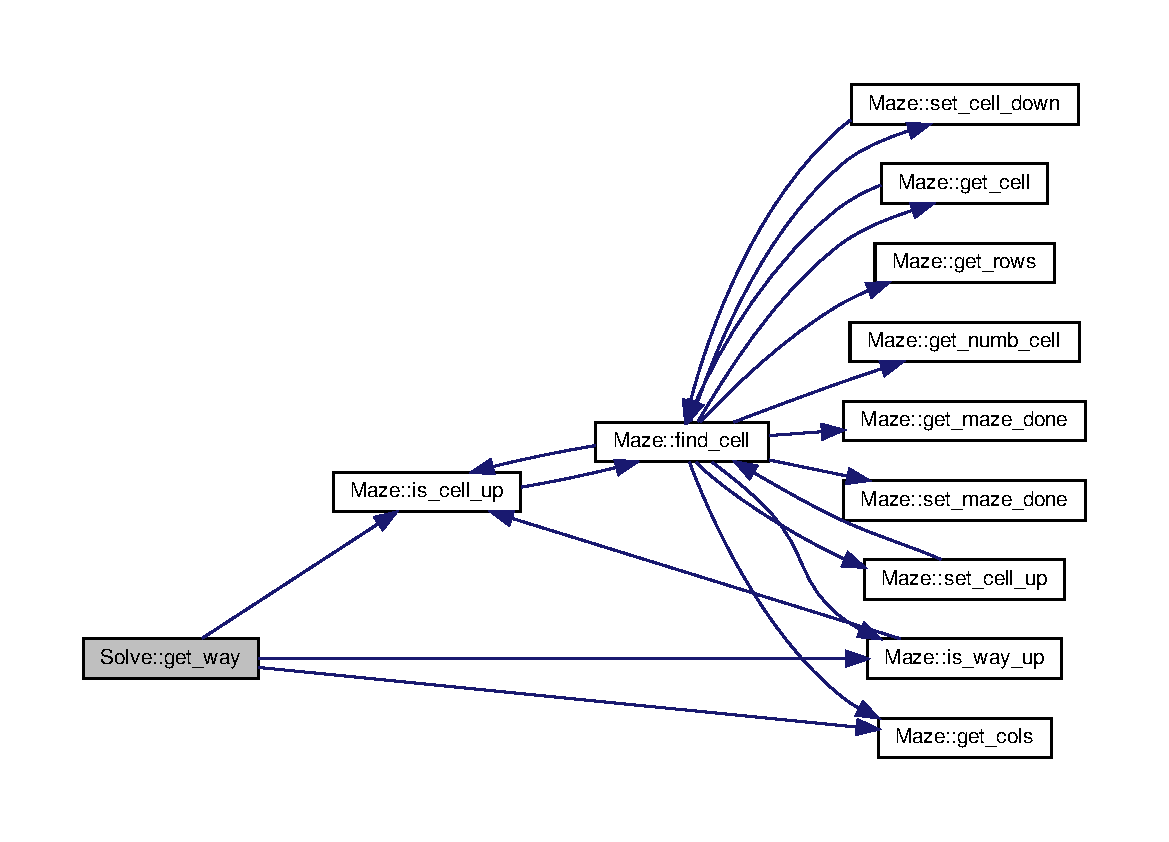
\includegraphics[width=350pt]{classSolve_a963b593c0311f03c7e4ce77eea818fa1_cgraph}
\end{center}
\end{figure}
Here is the caller graph for this function\+:\nopagebreak
\begin{figure}[H]
\begin{center}
\leavevmode
\includegraphics[width=350pt]{classSolve_a963b593c0311f03c7e4ce77eea818fa1_icgraph}
\end{center}
\end{figure}
\mbox{\Hypertarget{classSolve_aaccff68d3e175f7400a9407077db7255}\label{classSolve_aaccff68d3e175f7400a9407077db7255}} 
\index{Solve@{Solve}!get\+\_\+way\+\_\+numb@{get\+\_\+way\+\_\+numb}}
\index{get\+\_\+way\+\_\+numb@{get\+\_\+way\+\_\+numb}!Solve@{Solve}}
\subsubsection{\texorpdfstring{get\+\_\+way\+\_\+numb()}{get\_way\_numb()}}
{\footnotesize\ttfamily int Solve\+::get\+\_\+way\+\_\+numb (\begin{DoxyParamCaption}\item[{void}]{ }\end{DoxyParamCaption})}



! Method to get numbers of posible ways 

\begin{DoxyReturn}{Returns}
int numbers of ways. 
\end{DoxyReturn}

\begin{DoxyCode}
39 \{
40     m\_numb\_way = 0;
41     \textcolor{keywordflow}{if}( !m\_maze->\hyperlink{classMaze_a2b0e69e72d6c3e1037578f057946a21e}{is\_cell\_up}( m\_cell\_player, \hyperlink{classMaze_a07167e321eac2b67100fb82ecb98f1d1ab28354b543375bfa94dabaeda722927f}{Maze::status\_cell::top}) &&
42             !m\_maze->\hyperlink{classMaze_a308fa695665de6217c0e7f28aab5adda}{is\_way\_up}(m\_cell\_player - m\_maze->\hyperlink{classMaze_a8a04cd1335e96a80358181afa164d4c9}{get\_cols}()))
43     \{
44         m\_numb\_way++;
45     \}
46     \textcolor{keywordflow}{if}( !m\_maze->\hyperlink{classMaze_a2b0e69e72d6c3e1037578f057946a21e}{is\_cell\_up}( m\_cell\_player, \hyperlink{classMaze_a07167e321eac2b67100fb82ecb98f1d1a811882fecd5c7618d7099ebbd39ea254}{Maze::status\_cell::left}) &&
47             !m\_maze->\hyperlink{classMaze_a308fa695665de6217c0e7f28aab5adda}{is\_way\_up}( m\_cell\_player - 1))
48     \{
49         m\_numb\_way++;
50     \}
51     \textcolor{keywordflow}{if}( !m\_maze->\hyperlink{classMaze_a2b0e69e72d6c3e1037578f057946a21e}{is\_cell\_up}( m\_cell\_player, \hyperlink{classMaze_a07167e321eac2b67100fb82ecb98f1d1a74e8333ad11685ff3bdae589c8f6e34d}{Maze::status\_cell::down}) &&
52             !m\_maze->\hyperlink{classMaze_a308fa695665de6217c0e7f28aab5adda}{is\_way\_up}( m\_cell\_player + m\_maze->\hyperlink{classMaze_a8a04cd1335e96a80358181afa164d4c9}{get\_cols}()))
53     \{
54         m\_numb\_way++;
55     \}
56     \textcolor{keywordflow}{if}( !m\_maze->\hyperlink{classMaze_a2b0e69e72d6c3e1037578f057946a21e}{is\_cell\_up}( m\_cell\_player, \hyperlink{classMaze_a07167e321eac2b67100fb82ecb98f1d1a7c4f29407893c334a6cb7a87bf045c0d}{Maze::status\_cell::right}) &&
57             !m\_maze->\hyperlink{classMaze_a308fa695665de6217c0e7f28aab5adda}{is\_way\_up}( m\_cell\_player + 1))
58     \{
59         m\_numb\_way++;
60     \}
61     \textcolor{keywordflow}{return} m\_numb\_way;
62 \}
\end{DoxyCode}
Here is the call graph for this function\+:\nopagebreak
\begin{figure}[H]
\begin{center}
\leavevmode
\includegraphics[width=350pt]{classSolve_aaccff68d3e175f7400a9407077db7255_cgraph}
\end{center}
\end{figure}
Here is the caller graph for this function\+:\nopagebreak
\begin{figure}[H]
\begin{center}
\leavevmode
\includegraphics[width=350pt]{classSolve_aaccff68d3e175f7400a9407077db7255_icgraph}
\end{center}
\end{figure}
\mbox{\Hypertarget{classSolve_a868db181d288fdb10e5592b62e669c3b}\label{classSolve_a868db181d288fdb10e5592b62e669c3b}} 
\index{Solve@{Solve}!is\+\_\+done@{is\+\_\+done}}
\index{is\+\_\+done@{is\+\_\+done}!Solve@{Solve}}
\subsubsection{\texorpdfstring{is\+\_\+done()}{is\_done()}}
{\footnotesize\ttfamily bool Solve\+::is\+\_\+done (\begin{DoxyParamCaption}\item[{void}]{ }\end{DoxyParamCaption})}



! Method to check if the maze is Done 

\begin{DoxyReturn}{Returns}
True if the Cell Player are the last one. 
\end{DoxyReturn}

\begin{DoxyCode}
5 \{
6     \textcolor{keywordflow}{if}( m\_cell\_player == m\_maze->\hyperlink{classMaze_a90f5c1c140a9991942204d4a7fec3bf8}{get\_numb\_cell}()-1 )
7     \{
8 
9         m\_maze->\hyperlink{classMaze_aa7c832a91a3db8f48b31f688332f8986}{set\_cell\_up}( m\_cell\_player , \hyperlink{classMaze_a07167e321eac2b67100fb82ecb98f1d1ac83b72dd001482ce10f0b106c7a0ed0e}{Maze::status\_cell::way} );
10         \textcolor{keywordflow}{return} \textcolor{keyword}{true};
11     \}
12     \textcolor{keywordflow}{return} \textcolor{keyword}{false};
13 \}
\end{DoxyCode}
Here is the call graph for this function\+:\nopagebreak
\begin{figure}[H]
\begin{center}
\leavevmode
\includegraphics[width=350pt]{classSolve_a868db181d288fdb10e5592b62e669c3b_cgraph}
\end{center}
\end{figure}
Here is the caller graph for this function\+:\nopagebreak
\begin{figure}[H]
\begin{center}
\leavevmode
\includegraphics[width=350pt]{classSolve_a868db181d288fdb10e5592b62e669c3b_icgraph}
\end{center}
\end{figure}
\mbox{\Hypertarget{classSolve_a8902b46862c7759928495e3684054f82}\label{classSolve_a8902b46862c7759928495e3684054f82}} 
\index{Solve@{Solve}!move@{move}}
\index{move@{move}!Solve@{Solve}}
\subsubsection{\texorpdfstring{move()}{move()}}
{\footnotesize\ttfamily void Solve\+::move (\begin{DoxyParamCaption}\item[{void}]{ }\end{DoxyParamCaption})}



! Move to the next Cell backtrack. 


\begin{DoxyCode}
65 \{
66     \textcolor{keywordflow}{if}(\hyperlink{classSolve_aaccff68d3e175f7400a9407077db7255}{get\_way\_numb}() > 0 )
67     \{
68         \hyperlink{classSolve_a963b593c0311f03c7e4ce77eea818fa1}{get\_way}();
69         m\_stack\_cell.push(m\_cell\_player);
70         m\_maze->\hyperlink{classMaze_aa7c832a91a3db8f48b31f688332f8986}{set\_cell\_up}( m\_stack\_cell.top() , 
      \hyperlink{classMaze_a07167e321eac2b67100fb82ecb98f1d1ac83b72dd001482ce10f0b106c7a0ed0e}{Maze::status\_cell::way} );
71 
72         \textcolor{keywordflow}{if}(m\_stack\_ways.top() == 1)
73         \{
74             m\_cell\_player -= m\_maze->\hyperlink{classMaze_a8a04cd1335e96a80358181afa164d4c9}{get\_cols}();
75             m\_stack\_ways.pop();
76 
77         \}
78         \textcolor{keywordflow}{else} \textcolor{keywordflow}{if}(m\_stack\_ways.top() == 2)
79         \{
80             m\_cell\_player -= 1;
81             m\_stack\_ways.pop();
82         \}
83         \textcolor{keywordflow}{else} \textcolor{keywordflow}{if}(m\_stack\_ways.top() == 3)
84         \{
85             m\_cell\_player += m\_maze->\hyperlink{classMaze_a8a04cd1335e96a80358181afa164d4c9}{get\_cols}();
86             m\_stack\_ways.pop();
87 
88         \}
89         \textcolor{keywordflow}{else} \textcolor{keywordflow}{if}(m\_stack\_ways.top() == 4)
90         \{
91             m\_cell\_player += 1;
92             m\_stack\_ways.pop();
93         \}
94     \}
95     \textcolor{keywordflow}{else}
96     \{
97 
98         m\_maze->\hyperlink{classMaze_aa7c832a91a3db8f48b31f688332f8986}{set\_cell\_up}( m\_cell\_player, 
      \hyperlink{classMaze_a07167e321eac2b67100fb82ecb98f1d1a94708897ec9db8647dfe695714c98e46}{Maze::status\_cell::discarded} );
99         \textcolor{keywordflow}{if}( m\_maze->\hyperlink{classMaze_a2b0e69e72d6c3e1037578f057946a21e}{is\_cell\_up}( m\_cell\_player, \hyperlink{classMaze_a07167e321eac2b67100fb82ecb98f1d1ac83b72dd001482ce10f0b106c7a0ed0e}{Maze::status\_cell::way}))
100         \{
101             m\_maze->\hyperlink{classMaze_ab86292a84aa56a26c4c07f4aa684d9bb}{set\_cell\_down}(m\_cell\_player, 
      \hyperlink{classMaze_a07167e321eac2b67100fb82ecb98f1d1ac83b72dd001482ce10f0b106c7a0ed0e}{Maze::status\_cell::way});
102         \}
103         m\_cell\_player = m\_stack\_cell.top();
104         m\_stack\_cell.pop();
105         \textcolor{keywordflow}{while}( m\_stack\_ways.empty() )
106         \{
107             m\_stack\_ways.pop();
108         \}
109     \}
110 
111 \}
\end{DoxyCode}
Here is the call graph for this function\+:\nopagebreak
\begin{figure}[H]
\begin{center}
\leavevmode
\includegraphics[width=350pt]{classSolve_a8902b46862c7759928495e3684054f82_cgraph}
\end{center}
\end{figure}
Here is the caller graph for this function\+:\nopagebreak
\begin{figure}[H]
\begin{center}
\leavevmode
\includegraphics[width=350pt]{classSolve_a8902b46862c7759928495e3684054f82_icgraph}
\end{center}
\end{figure}
\mbox{\Hypertarget{classSolve_a8226032eb1d4877539f417d4fab0efde}\label{classSolve_a8226032eb1d4877539f417d4fab0efde}} 
\index{Solve@{Solve}!move\+\_\+left@{move\+\_\+left}}
\index{move\+\_\+left@{move\+\_\+left}!Solve@{Solve}}
\subsubsection{\texorpdfstring{move\+\_\+left()}{move\_left()}}
{\footnotesize\ttfamily bool Solve\+::move\+\_\+left (\begin{DoxyParamCaption}\item[{void}]{ }\end{DoxyParamCaption})}



! Move to the next cell left hand. 

if Left hand have wall and front wall is not up and cell in front is not way and not discarted. 
\begin{DoxyCode}
114 \{
115     \textcolor{keywordflow}{switch} (front)
116     \{
117         \textcolor{keywordflow}{case} 1:
118             \textcolor{keywordflow}{if}( m\_maze->\hyperlink{classMaze_a2b0e69e72d6c3e1037578f057946a21e}{is\_cell\_up}( m\_cell\_player, 
      \hyperlink{classMaze_a07167e321eac2b67100fb82ecb98f1d1a811882fecd5c7618d7099ebbd39ea254}{Maze::status\_cell::left} ) &&
119                     !m\_maze->\hyperlink{classMaze_a2b0e69e72d6c3e1037578f057946a21e}{is\_cell\_up}( m\_cell\_player, 
      \hyperlink{classMaze_a07167e321eac2b67100fb82ecb98f1d1ab28354b543375bfa94dabaeda722927f}{Maze::status\_cell::top}) &&
120                     !m\_maze->\hyperlink{classMaze_a308fa695665de6217c0e7f28aab5adda}{is\_way\_up}( m\_cell\_player - m\_maze->
      \hyperlink{classMaze_a8a04cd1335e96a80358181afa164d4c9}{get\_cols}() ))
121             \{
122                 Turners = 0;
123                 m\_maze->\hyperlink{classMaze_aa7c832a91a3db8f48b31f688332f8986}{set\_cell\_up}( m\_cell\_player , 
      \hyperlink{classMaze_a07167e321eac2b67100fb82ecb98f1d1ac83b72dd001482ce10f0b106c7a0ed0e}{Maze::status\_cell::way} );
124                 m\_cell\_player -= m\_maze->\hyperlink{classMaze_a8a04cd1335e96a80358181afa164d4c9}{get\_cols}();
125                 \textcolor{keywordflow}{return} \textcolor{keyword}{true};
126             \}
127             \textcolor{keywordflow}{else}
128             \{
129                 \textcolor{keywordflow}{if}( !m\_maze->\hyperlink{classMaze_a2b0e69e72d6c3e1037578f057946a21e}{is\_cell\_up}( m\_cell\_player, 
      \hyperlink{classMaze_a07167e321eac2b67100fb82ecb98f1d1a811882fecd5c7618d7099ebbd39ea254}{Maze::status\_cell::left} )) 
130                 \{
131                     Turners = 0;
132                     front = 4;
133                     hand = 3;
134                     m\_maze->\hyperlink{classMaze_aa7c832a91a3db8f48b31f688332f8986}{set\_cell\_up}( m\_cell\_player , 
      \hyperlink{classMaze_a07167e321eac2b67100fb82ecb98f1d1ac83b72dd001482ce10f0b106c7a0ed0e}{Maze::status\_cell::way} );
135                     m\_cell\_player -= 1;
136                     \textcolor{keywordflow}{return} \textcolor{keyword}{true};
137                 \}
138                 \textcolor{keywordflow}{else}
139                 \{
140                     Turners++;
141                     front = 2;
142                     hand = 1;
143                 \}
144                 \textcolor{keywordflow}{break};
145             \}
146 
147         \textcolor{keywordflow}{case} 2:
148             \textcolor{keywordflow}{if}( m\_maze->\hyperlink{classMaze_a2b0e69e72d6c3e1037578f057946a21e}{is\_cell\_up}( m\_cell\_player, 
      \hyperlink{classMaze_a07167e321eac2b67100fb82ecb98f1d1ab28354b543375bfa94dabaeda722927f}{Maze::status\_cell::top} ) &&
149                     !m\_maze->\hyperlink{classMaze_a2b0e69e72d6c3e1037578f057946a21e}{is\_cell\_up}( m\_cell\_player, 
      \hyperlink{classMaze_a07167e321eac2b67100fb82ecb98f1d1a7c4f29407893c334a6cb7a87bf045c0d}{Maze::status\_cell::right}) && 
150                     !m\_maze->\hyperlink{classMaze_a308fa695665de6217c0e7f28aab5adda}{is\_way\_up}( m\_cell\_player+1 ))
151             \{
152                 Turners = 0;
153                 m\_maze->\hyperlink{classMaze_aa7c832a91a3db8f48b31f688332f8986}{set\_cell\_up}( m\_cell\_player , 
      \hyperlink{classMaze_a07167e321eac2b67100fb82ecb98f1d1ac83b72dd001482ce10f0b106c7a0ed0e}{Maze::status\_cell::way} );
154                 m\_cell\_player += 1;
155                 \textcolor{keywordflow}{return} \textcolor{keyword}{true};
156             \}
157             \textcolor{keywordflow}{else}
158             \{
159                 \textcolor{keywordflow}{if}( !m\_maze->\hyperlink{classMaze_a2b0e69e72d6c3e1037578f057946a21e}{is\_cell\_up}( m\_cell\_player, 
      \hyperlink{classMaze_a07167e321eac2b67100fb82ecb98f1d1ab28354b543375bfa94dabaeda722927f}{Maze::status\_cell::top} ))
160                 \{
161                     Turners = 0;
162                     front = 1;
163                     hand = 4;
164                     m\_maze->\hyperlink{classMaze_aa7c832a91a3db8f48b31f688332f8986}{set\_cell\_up}( m\_cell\_player , 
      \hyperlink{classMaze_a07167e321eac2b67100fb82ecb98f1d1ac83b72dd001482ce10f0b106c7a0ed0e}{Maze::status\_cell::way} );
165                     m\_cell\_player -= m\_maze->\hyperlink{classMaze_a8a04cd1335e96a80358181afa164d4c9}{get\_cols}();
166                     \textcolor{keywordflow}{return} \textcolor{keyword}{true};
167                 \}
168                 \textcolor{keywordflow}{else}
169                 \{
170                     Turners++;
171                     front = 3;
172                     hand = 2;
173                 \}
174                 \textcolor{keywordflow}{break};
175             \}
176         \textcolor{keywordflow}{case} 3:
177             \textcolor{keywordflow}{if}(     m\_maze->\hyperlink{classMaze_a2b0e69e72d6c3e1037578f057946a21e}{is\_cell\_up}( m\_cell\_player, 
      \hyperlink{classMaze_a07167e321eac2b67100fb82ecb98f1d1a7c4f29407893c334a6cb7a87bf045c0d}{Maze::status\_cell::right} ) &&
178                     !m\_maze->\hyperlink{classMaze_a2b0e69e72d6c3e1037578f057946a21e}{is\_cell\_up}( m\_cell\_player, 
      \hyperlink{classMaze_a07167e321eac2b67100fb82ecb98f1d1a74e8333ad11685ff3bdae589c8f6e34d}{Maze::status\_cell::down}) &&
179                     !m\_maze->\hyperlink{classMaze_a308fa695665de6217c0e7f28aab5adda}{is\_way\_up}( m\_cell\_player+m\_maze->\hyperlink{classMaze_a8a04cd1335e96a80358181afa164d4c9}{get\_cols}() ))
180             \{
181                 Turners = 0;
182                 m\_maze->\hyperlink{classMaze_aa7c832a91a3db8f48b31f688332f8986}{set\_cell\_up}( m\_cell\_player , 
      \hyperlink{classMaze_a07167e321eac2b67100fb82ecb98f1d1ac83b72dd001482ce10f0b106c7a0ed0e}{Maze::status\_cell::way} );
183                 m\_cell\_player += m\_maze->\hyperlink{classMaze_a8a04cd1335e96a80358181afa164d4c9}{get\_cols}();
184                 \textcolor{keywordflow}{return} \textcolor{keyword}{true};
185             \}
186             \textcolor{keywordflow}{else}
187             \{
188 
189                 \textcolor{keywordflow}{if}( !m\_maze->\hyperlink{classMaze_a2b0e69e72d6c3e1037578f057946a21e}{is\_cell\_up}( m\_cell\_player, 
      \hyperlink{classMaze_a07167e321eac2b67100fb82ecb98f1d1a7c4f29407893c334a6cb7a87bf045c0d}{Maze::status\_cell::right} ))
190                 \{
191                     Turners = 0;
192                     front = 2;
193                     hand = 1;
194                     m\_maze->\hyperlink{classMaze_aa7c832a91a3db8f48b31f688332f8986}{set\_cell\_up}( m\_cell\_player , 
      \hyperlink{classMaze_a07167e321eac2b67100fb82ecb98f1d1ac83b72dd001482ce10f0b106c7a0ed0e}{Maze::status\_cell::way} );
195                     m\_cell\_player += 1;
196                     \textcolor{keywordflow}{return} \textcolor{keyword}{true};
197                 \}
198                 \textcolor{keywordflow}{else}
199                 \{
200                     Turners++;
201                     front = 4;
202                     hand = 3;
203                 \}
204                 \textcolor{keywordflow}{break};
205             \}
206 
207         \textcolor{keywordflow}{case} 4:
209             \textcolor{keywordflow}{if}(     m\_maze->\hyperlink{classMaze_a2b0e69e72d6c3e1037578f057946a21e}{is\_cell\_up}( m\_cell\_player, 
      \hyperlink{classMaze_a07167e321eac2b67100fb82ecb98f1d1a74e8333ad11685ff3bdae589c8f6e34d}{Maze::status\_cell::down} ) &&
210                     !m\_maze->\hyperlink{classMaze_a2b0e69e72d6c3e1037578f057946a21e}{is\_cell\_up}( m\_cell\_player, 
      \hyperlink{classMaze_a07167e321eac2b67100fb82ecb98f1d1a811882fecd5c7618d7099ebbd39ea254}{Maze::status\_cell::left}) &&
211                     !m\_maze->\hyperlink{classMaze_a308fa695665de6217c0e7f28aab5adda}{is\_way\_up}( m\_cell\_player-1))
212             \{
213                 Turners = 0;
214                 m\_maze->\hyperlink{classMaze_aa7c832a91a3db8f48b31f688332f8986}{set\_cell\_up}( m\_cell\_player , 
      \hyperlink{classMaze_a07167e321eac2b67100fb82ecb98f1d1ac83b72dd001482ce10f0b106c7a0ed0e}{Maze::status\_cell::way} );
215                 m\_cell\_player -= 1;
216                 \textcolor{keywordflow}{return} \textcolor{keyword}{true};
217             \}\textcolor{keywordflow}{else}
218             \{
219                 \textcolor{comment}{// if not have wall on left.}
220                 \textcolor{keywordflow}{if}( !m\_maze->\hyperlink{classMaze_a2b0e69e72d6c3e1037578f057946a21e}{is\_cell\_up}( m\_cell\_player, 
      \hyperlink{classMaze_a07167e321eac2b67100fb82ecb98f1d1a74e8333ad11685ff3bdae589c8f6e34d}{Maze::status\_cell::down}))
221                 \{
222                     Turners = 0;
223                     front = 3;
224                     hand = 2;
225                     m\_maze->\hyperlink{classMaze_aa7c832a91a3db8f48b31f688332f8986}{set\_cell\_up}( m\_cell\_player , 
      \hyperlink{classMaze_a07167e321eac2b67100fb82ecb98f1d1ac83b72dd001482ce10f0b106c7a0ed0e}{Maze::status\_cell::way} );
226                     m\_cell\_player += m\_maze->\hyperlink{classMaze_a8a04cd1335e96a80358181afa164d4c9}{get\_cols}();
227                     \textcolor{keywordflow}{return} \textcolor{keyword}{true};
228                 \}
229                 \textcolor{keywordflow}{else}
230                 \{
231                     Turners++;
232                     front = 1;
233                     hand = 4;
234                 \}
235                 \textcolor{keywordflow}{break};
236             \}
237     \}
238 
239     \textcolor{keywordflow}{return} \textcolor{keyword}{false};
240 \}
\end{DoxyCode}
Here is the call graph for this function\+:\nopagebreak
\begin{figure}[H]
\begin{center}
\leavevmode
\includegraphics[width=350pt]{classSolve_a8226032eb1d4877539f417d4fab0efde_cgraph}
\end{center}
\end{figure}
Here is the caller graph for this function\+:\nopagebreak
\begin{figure}[H]
\begin{center}
\leavevmode
\includegraphics[width=350pt]{classSolve_a8226032eb1d4877539f417d4fab0efde_icgraph}
\end{center}
\end{figure}
\mbox{\Hypertarget{classSolve_a2c0330bee4d1cafc5b3c7d5f7ba72697}\label{classSolve_a2c0330bee4d1cafc5b3c7d5f7ba72697}} 
\index{Solve@{Solve}!operator=@{operator=}}
\index{operator=@{operator=}!Solve@{Solve}}
\subsubsection{\texorpdfstring{operator=()}{operator=()}}
{\footnotesize\ttfamily \hyperlink{classSolve}{Solve}\& Solve\+::operator= (\begin{DoxyParamCaption}\item[{const \hyperlink{classSolve}{Solve} \&}]{s }\end{DoxyParamCaption})\hspace{0.3cm}{\ttfamily [inline]}}



! Assignment operator. 


\begin{DoxyCode}
56         \{
57             this->m\_maze = s.m\_maze;
58             this->m\_stack\_cell = s.m\_stack\_cell;
59             this->m\_stack\_ways = s.m\_stack\_ways;
60             this->m\_cell\_player = s.m\_cell\_player;
61             this->m\_numb\_way = s.m\_numb\_way;
62 
63             \textcolor{keywordflow}{return} *\textcolor{keyword}{this};
64         \}
\end{DoxyCode}
Here is the call graph for this function\+:\nopagebreak
\begin{figure}[H]
\begin{center}
\leavevmode
\includegraphics[width=350pt]{classSolve_a2c0330bee4d1cafc5b3c7d5f7ba72697_cgraph}
\end{center}
\end{figure}


The documentation for this class was generated from the following files\+:\begin{DoxyCompactItemize}
\item 
/home/bergony/lp\+\_\+magos/include/\hyperlink{solve_8h}{solve.\+h}\item 
/home/bergony/lp\+\_\+magos/src/\hyperlink{solve_8cpp}{solve.\+cpp}\end{DoxyCompactItemize}

\chapter{File Documentation}
\hypertarget{build_8h}{}\section{/home/bergony/lp\+\_\+magos/include/build.h File Reference}
\label{build_8h}\index{/home/bergony/lp\+\_\+magos/include/build.\+h@{/home/bergony/lp\+\_\+magos/include/build.\+h}}
{\ttfamily \#include $<$set$>$}\newline
{\ttfamily \#include \char`\"{}maze.\+h\char`\"{}}\newline
Include dependency graph for build.\+h\+:\nopagebreak
\begin{figure}[H]
\begin{center}
\leavevmode
\includegraphics[width=256pt]{build_8h__incl}
\end{center}
\end{figure}
This graph shows which files directly or indirectly include this file\+:\nopagebreak
\begin{figure}[H]
\begin{center}
\leavevmode
\includegraphics[width=350pt]{build_8h__dep__incl}
\end{center}
\end{figure}
\subsection*{Classes}
\begin{DoxyCompactItemize}
\item 
class \hyperlink{classBuild}{Build}
\begin{DoxyCompactList}\small\item\em {\bfseries Class} \hyperlink{classBuild}{Build} {\itshape Class that recives a \hyperlink{classMaze}{Maze} to be \hyperlink{classBuild}{Build}.} \end{DoxyCompactList}\end{DoxyCompactItemize}

\hypertarget{canvas_8h}{}\section{/home/bergony/lp\+\_\+magos/include/canvas.h File Reference}
\label{canvas_8h}\index{/home/bergony/lp\+\_\+magos/include/canvas.\+h@{/home/bergony/lp\+\_\+magos/include/canvas.\+h}}
{\ttfamily \#include $<$cstring$>$}\newline
{\ttfamily \#include $<$stdio.\+h$>$}\newline
Include dependency graph for canvas.\+h\+:\nopagebreak
\begin{figure}[H]
\begin{center}
\leavevmode
\includegraphics[width=206pt]{canvas_8h__incl}
\end{center}
\end{figure}
This graph shows which files directly or indirectly include this file\+:\nopagebreak
\begin{figure}[H]
\begin{center}
\leavevmode
\includegraphics[width=350pt]{canvas_8h__dep__incl}
\end{center}
\end{figure}
\subsection*{Classes}
\begin{DoxyCompactItemize}
\item 
struct \hyperlink{structColor}{Color}
\begin{DoxyCompactList}\small\item\em {\bfseries Struct} \hyperlink{structColor}{Color} {\itshape  \hyperlink{structColor}{Color} of to printer.} \end{DoxyCompactList}\item 
class \hyperlink{classCanvas}{Canvas}
\begin{DoxyCompactList}\small\item\em {\bfseries Class} \hyperlink{classCanvas}{Canvas} {\itshape Class to creates a \hyperlink{classCanvas}{Canvas} to be draw( Line and Box ).} \end{DoxyCompactList}\end{DoxyCompactItemize}
\subsection*{Typedefs}
\begin{DoxyCompactItemize}
\item 
typedef unsigned char \hyperlink{canvas_8h_a0c8186d9b9b7880309c27230bbb5e69d}{byte}
\end{DoxyCompactItemize}


\subsection{Typedef Documentation}
\mbox{\Hypertarget{canvas_8h_a0c8186d9b9b7880309c27230bbb5e69d}\label{canvas_8h_a0c8186d9b9b7880309c27230bbb5e69d}} 
\index{canvas.\+h@{canvas.\+h}!byte@{byte}}
\index{byte@{byte}!canvas.\+h@{canvas.\+h}}
\subsubsection{\texorpdfstring{byte}{byte}}
{\footnotesize\ttfamily typedef unsigned char \hyperlink{canvas_8h_a0c8186d9b9b7880309c27230bbb5e69d}{byte}}


\hypertarget{game__loop_8h}{}\section{/home/bergony/lp\+\_\+magos/include/game\+\_\+loop.h File Reference}
\label{game__loop_8h}\index{/home/bergony/lp\+\_\+magos/include/game\+\_\+loop.\+h@{/home/bergony/lp\+\_\+magos/include/game\+\_\+loop.\+h}}
{\ttfamily \#include \char`\"{}../include/build.\+h\char`\"{}}\newline
{\ttfamily \#include \char`\"{}../include/render.\+h\char`\"{}}\newline
{\ttfamily \#include \char`\"{}../include/solve.\+h\char`\"{}}\newline
Include dependency graph for game\+\_\+loop.\+h\+:\nopagebreak
\begin{figure}[H]
\begin{center}
\leavevmode
\includegraphics[width=350pt]{game__loop_8h__incl}
\end{center}
\end{figure}
This graph shows which files directly or indirectly include this file\+:\nopagebreak
\begin{figure}[H]
\begin{center}
\leavevmode
\includegraphics[width=350pt]{game__loop_8h__dep__incl}
\end{center}
\end{figure}
\subsection*{Classes}
\begin{DoxyCompactItemize}
\item 
class \hyperlink{classGame__Loop}{Game\+\_\+\+Loop}
\begin{DoxyCompactList}\small\item\em {\bfseries Class} Game\+\_\+loop {\itshape Class to control output. input and end of game.} \end{DoxyCompactList}\end{DoxyCompactItemize}

\hypertarget{maze_8h}{}\section{/home/bergony/lp\+\_\+magos/include/maze.h File Reference}
\label{maze_8h}\index{/home/bergony/lp\+\_\+magos/include/maze.\+h@{/home/bergony/lp\+\_\+magos/include/maze.\+h}}
{\ttfamily \#include $<$iostream$>$}\newline
{\ttfamily \#include $<$vector$>$}\newline
{\ttfamily \#include $<$bitset$>$}\newline
Include dependency graph for maze.\+h\+:\nopagebreak
\begin{figure}[H]
\begin{center}
\leavevmode
\includegraphics[width=256pt]{maze_8h__incl}
\end{center}
\end{figure}
This graph shows which files directly or indirectly include this file\+:\nopagebreak
\begin{figure}[H]
\begin{center}
\leavevmode
\includegraphics[width=350pt]{maze_8h__dep__incl}
\end{center}
\end{figure}
\subsection*{Classes}
\begin{DoxyCompactItemize}
\item 
class \hyperlink{classMaze}{Maze}
\begin{DoxyCompactList}\small\item\em {\bfseries Class} \hyperlink{classMaze}{Maze} {\itshape Class create a \hyperlink{classMaze}{Maze} to be \hyperlink{classBuild}{Build}, \hyperlink{classSolve}{Solve} and \hyperlink{classRender}{Render}.} \end{DoxyCompactList}\end{DoxyCompactItemize}
\subsection*{Typedefs}
\begin{DoxyCompactItemize}
\item 
typedef unsigned char \hyperlink{maze_8h_a789d352559efaa396a258805d44f4289}{bit}
\begin{DoxyCompactList}\small\item\em to use as a bit. \end{DoxyCompactList}\end{DoxyCompactItemize}


\subsection{Typedef Documentation}
\mbox{\Hypertarget{maze_8h_a789d352559efaa396a258805d44f4289}\label{maze_8h_a789d352559efaa396a258805d44f4289}} 
\index{maze.\+h@{maze.\+h}!bit@{bit}}
\index{bit@{bit}!maze.\+h@{maze.\+h}}
\subsubsection{\texorpdfstring{bit}{bit}}
{\footnotesize\ttfamily typedef unsigned char \hyperlink{maze_8h_a789d352559efaa396a258805d44f4289}{bit}}



to use as a bit. 


\hypertarget{render_8h}{}\section{/home/bergony/lp\+\_\+magos/include/render.h File Reference}
\label{render_8h}\index{/home/bergony/lp\+\_\+magos/include/render.\+h@{/home/bergony/lp\+\_\+magos/include/render.\+h}}
{\ttfamily \#include \char`\"{}../include/canvas.\+h\char`\"{}}\newline
{\ttfamily \#include \char`\"{}../include/maze.\+h\char`\"{}}\newline
{\ttfamily \#include $<$string$>$}\newline
Include dependency graph for render.\+h\+:\nopagebreak
\begin{figure}[H]
\begin{center}
\leavevmode
\includegraphics[width=350pt]{render_8h__incl}
\end{center}
\end{figure}
This graph shows which files directly or indirectly include this file\+:\nopagebreak
\begin{figure}[H]
\begin{center}
\leavevmode
\includegraphics[width=350pt]{render_8h__dep__incl}
\end{center}
\end{figure}
\subsection*{Classes}
\begin{DoxyCompactItemize}
\item 
class \hyperlink{classRender}{Render}
\begin{DoxyCompactList}\small\item\em {\bfseries Class} \hyperlink{classRender}{Render} {\itshape A class that recive \hyperlink{classMaze}{Maze} Object to draw in the \hyperlink{classCanvas}{Canvas}.} \end{DoxyCompactList}\end{DoxyCompactItemize}

\hypertarget{solve_8h}{}\section{/home/bergony/lp\+\_\+magos/include/solve.h File Reference}
\label{solve_8h}\index{/home/bergony/lp\+\_\+magos/include/solve.\+h@{/home/bergony/lp\+\_\+magos/include/solve.\+h}}
{\ttfamily \#include $<$stack$>$}\newline
{\ttfamily \#include \char`\"{}../include/maze.\+h\char`\"{}}\newline
Include dependency graph for solve.\+h\+:\nopagebreak
\begin{figure}[H]
\begin{center}
\leavevmode
\includegraphics[width=268pt]{solve_8h__incl}
\end{center}
\end{figure}
This graph shows which files directly or indirectly include this file\+:\nopagebreak
\begin{figure}[H]
\begin{center}
\leavevmode
\includegraphics[width=350pt]{solve_8h__dep__incl}
\end{center}
\end{figure}
\subsection*{Classes}
\begin{DoxyCompactItemize}
\item 
class \hyperlink{classSolve}{Solve}
\begin{DoxyCompactList}\small\item\em {\bfseries Class} \hyperlink{classSolve}{Solve} {\itshape Class that recive a \hyperlink{classMaze}{Maze} to be \hyperlink{classSolve}{Solve}.} \end{DoxyCompactList}\end{DoxyCompactItemize}
\subsection*{Typedefs}
\begin{DoxyCompactItemize}
\item 
typedef unsigned char \hyperlink{solve_8h_a789d352559efaa396a258805d44f4289}{bit}
\end{DoxyCompactItemize}


\subsection{Typedef Documentation}
\mbox{\Hypertarget{solve_8h_a789d352559efaa396a258805d44f4289}\label{solve_8h_a789d352559efaa396a258805d44f4289}} 
\index{solve.\+h@{solve.\+h}!bit@{bit}}
\index{bit@{bit}!solve.\+h@{solve.\+h}}
\subsubsection{\texorpdfstring{bit}{bit}}
{\footnotesize\ttfamily typedef unsigned char \hyperlink{maze_8h_a789d352559efaa396a258805d44f4289}{bit}}


\hypertarget{build_8cpp}{}\section{/home/bergony/lp\+\_\+magos/src/build.cpp File Reference}
\label{build_8cpp}\index{/home/bergony/lp\+\_\+magos/src/build.\+cpp@{/home/bergony/lp\+\_\+magos/src/build.\+cpp}}
{\ttfamily \#include \char`\"{}../include/build.\+h\char`\"{}}\newline
{\ttfamily \#include $<$stdlib.\+h$>$}\newline
{\ttfamily \#include $<$ctime$>$}\newline
Include dependency graph for build.\+cpp\+:\nopagebreak
\begin{figure}[H]
\begin{center}
\leavevmode
\includegraphics[width=315pt]{build_8cpp__incl}
\end{center}
\end{figure}

\hypertarget{canvas_8cpp}{}\section{/home/bergony/lp\+\_\+magos/src/canvas.cpp File Reference}
\label{canvas_8cpp}\index{/home/bergony/lp\+\_\+magos/src/canvas.\+cpp@{/home/bergony/lp\+\_\+magos/src/canvas.\+cpp}}
{\ttfamily \#include $<$cstring$>$}\newline
{\ttfamily \#include \char`\"{}../include/canvas.\+h\char`\"{}}\newline
Include dependency graph for canvas.\+cpp\+:\nopagebreak
\begin{figure}[H]
\begin{center}
\leavevmode
\includegraphics[width=232pt]{canvas_8cpp__incl}
\end{center}
\end{figure}

\hypertarget{game__loop_8cpp}{}\section{/home/bergony/lp\+\_\+magos/src/game\+\_\+loop.cpp File Reference}
\label{game__loop_8cpp}\index{/home/bergony/lp\+\_\+magos/src/game\+\_\+loop.\+cpp@{/home/bergony/lp\+\_\+magos/src/game\+\_\+loop.\+cpp}}
{\ttfamily \#include \char`\"{}../include/game\+\_\+loop.\+h\char`\"{}}\newline
{\ttfamily \#include $<$iomanip$>$}\newline
Include dependency graph for game\+\_\+loop.\+cpp\+:\nopagebreak
\begin{figure}[H]
\begin{center}
\leavevmode
\includegraphics[width=350pt]{game__loop_8cpp__incl}
\end{center}
\end{figure}

\hypertarget{main_8cpp}{}\section{/home/bergony/lp\+\_\+magos/src/main.cpp File Reference}
\label{main_8cpp}\index{/home/bergony/lp\+\_\+magos/src/main.\+cpp@{/home/bergony/lp\+\_\+magos/src/main.\+cpp}}
{\ttfamily \#include \char`\"{}../include/game\+\_\+loop.\+h\char`\"{}}\newline
Include dependency graph for main.\+cpp\+:\nopagebreak
\begin{figure}[H]
\begin{center}
\leavevmode
\includegraphics[width=350pt]{main_8cpp__incl}
\end{center}
\end{figure}
\subsection*{Functions}
\begin{DoxyCompactItemize}
\item 
int \hyperlink{main_8cpp_a3c04138a5bfe5d72780bb7e82a18e627}{main} (int argc, char $\ast$$\ast$argv)
\end{DoxyCompactItemize}


\subsection{Function Documentation}
\mbox{\Hypertarget{main_8cpp_a3c04138a5bfe5d72780bb7e82a18e627}\label{main_8cpp_a3c04138a5bfe5d72780bb7e82a18e627}} 
\index{main.\+cpp@{main.\+cpp}!main@{main}}
\index{main@{main}!main.\+cpp@{main.\+cpp}}
\subsubsection{\texorpdfstring{main()}{main()}}
{\footnotesize\ttfamily int main (\begin{DoxyParamCaption}\item[{int}]{argc,  }\item[{char $\ast$$\ast$}]{argv }\end{DoxyParamCaption})}

This is a \hyperlink{main_8cpp}{main.\+cpp} file here will be

place the Game\+Loop and the game.

\begin{DoxyAuthor}{Author}
Bergony Bandeira
\end{DoxyAuthor}
\begin{DoxyDate}{Date}
10/12/2018
\end{DoxyDate}

\begin{DoxyCode}
40 \{
41 
43 
52     \textcolor{keywordtype}{int} cols\{3\};            \textcolor{comment}{//   Default Value.}
53     \textcolor{keywordtype}{int} rows\{3\};            \textcolor{comment}{//   Default Value.}
54     \textcolor{keywordtype}{int} width\{100\};         \textcolor{comment}{//   Default Value.}
55     \textcolor{keywordtype}{int} height\{100\};        \textcolor{comment}{//   Default Value.}
56 
57     \textcolor{keywordflow}{switch} (argc)
58     \{
59         \textcolor{keywordflow}{case} 1:
60             std::cout << \textcolor{stringliteral}{"wrong argument numbers\(\backslash\)n"};
61             \textcolor{keywordflow}{return} -1;
62         \textcolor{keywordflow}{case} 2:
63             std::cout << \textcolor{stringliteral}{"wrong argument numbers\(\backslash\)n"};
64             \textcolor{keywordflow}{return} -1;
65         \textcolor{keywordflow}{case} 3:
66             std::cout << \textcolor{stringliteral}{"wrong argument numbers\(\backslash\)n"};
67             \textcolor{keywordflow}{return} -1;
68         \textcolor{keywordflow}{case} 4:
69             rows = atoi(argv[1]);
70             cols = atoi(argv[2]);
71             width = atoi(argv[3]);
72             height = (cols * width) / rows;
73             \textcolor{keywordflow}{break};
74         \textcolor{keywordflow}{case} 5:
75             rows = atoi(argv[1]);
76             cols = atoi(argv[2]);
77             width = atoi(argv[3]);
78             height = atoi(argv[4]);
79             \textcolor{keywordflow}{break};
80         \textcolor{keywordflow}{default}:
81             \textcolor{keywordflow}{break};
82     \}
83 
84     std::cout << \textcolor{stringliteral}{"============================ MAze Generator SOlve ================================"} << \textcolor{stringliteral}{"
      \(\backslash\)n"};
85     std::cout << \textcolor{stringliteral}{"Canvas Size "} << width << \textcolor{stringliteral}{" x "} << height << \textcolor{stringliteral}{"\(\backslash\)n"};
86     std::cout << \textcolor{stringliteral}{"Maze Size "} << rows << \textcolor{stringliteral}{" x "} << cols << \textcolor{stringliteral}{"\(\backslash\)n"};
87     \hyperlink{classGame__Loop}{Game\_Loop} gl( rows, cols, width, height );
88 
89     gl.initializer();
90 
91     \textcolor{keywordflow}{while}(!gl.done())
92     \{
93         gl.update();
94     \}
95 
96     \textcolor{keywordflow}{return} 0;
97 
98 \}
\end{DoxyCode}
Here is the call graph for this function\+:\nopagebreak
\begin{figure}[H]
\begin{center}
\leavevmode
\includegraphics[width=350pt]{main_8cpp_a3c04138a5bfe5d72780bb7e82a18e627_cgraph}
\end{center}
\end{figure}

\hypertarget{maze_8cpp}{}\section{/home/bergony/lp\+\_\+magos/src/maze.cpp File Reference}
\label{maze_8cpp}\index{/home/bergony/lp\+\_\+magos/src/maze.\+cpp@{/home/bergony/lp\+\_\+magos/src/maze.\+cpp}}
{\ttfamily \#include \char`\"{}../include/maze.\+h\char`\"{}}\newline
Include dependency graph for maze.\+cpp\+:\nopagebreak
\begin{figure}[H]
\begin{center}
\leavevmode
\includegraphics[width=256pt]{maze_8cpp__incl}
\end{center}
\end{figure}

\hypertarget{render_8cpp}{}\section{/home/bergony/lp\+\_\+magos/src/render.cpp File Reference}
\label{render_8cpp}\index{/home/bergony/lp\+\_\+magos/src/render.\+cpp@{/home/bergony/lp\+\_\+magos/src/render.\+cpp}}
{\ttfamily \#include \char`\"{}../include/stb\+\_\+image\+\_\+write.\+h\char`\"{}}\newline
{\ttfamily \#include \char`\"{}../include/render.\+h\char`\"{}}\newline
{\ttfamily \#include $<$string$>$}\newline
Include dependency graph for render.\+cpp\+:\nopagebreak
\begin{figure}[H]
\begin{center}
\leavevmode
\includegraphics[width=350pt]{render_8cpp__incl}
\end{center}
\end{figure}
\subsection*{Macros}
\begin{DoxyCompactItemize}
\item 
\#define \hyperlink{render_8cpp_aefe397a94e8feddc652f92ef40ce9597}{S\+T\+B\+\_\+\+I\+M\+A\+G\+E\+\_\+\+W\+R\+I\+T\+E\+\_\+\+I\+M\+P\+L\+E\+M\+E\+N\+T\+A\+T\+I\+ON}
\end{DoxyCompactItemize}
\subsection*{Variables}
\begin{DoxyCompactItemize}
\item 
const \hyperlink{structColor}{Color} \hyperlink{render_8cpp_a009fdb656a368e46b7d614e7438b5830}{G\+R\+AY} (200, 200, 200)
\item 
const \hyperlink{structColor}{Color} \hyperlink{render_8cpp_ada1558ae37a1ddfc6c8b784f809385d4}{B\+L\+A\+CK} (0, 0, 0)
\item 
const \hyperlink{structColor}{Color} \hyperlink{render_8cpp_a0db58550f21b0b45458ade7d071c3500}{R\+ED} (255, 0, 0)
\item 
const \hyperlink{structColor}{Color} \hyperlink{render_8cpp_a0616d169807ac93a808a3928d058d2d5}{Y\+E\+L\+L\+OW} (255, 255, 0)
\item 
const \hyperlink{structColor}{Color} \hyperlink{render_8cpp_a58d827358f6165cc5927d28b2dcff311}{G\+R\+E\+EN} (0, 0, 255)
\item 
const \hyperlink{structColor}{Color} \hyperlink{render_8cpp_ab49b84fe87ce8b46e7e4a25be82c7538}{B\+L\+UE} (0, 255, 0)
\end{DoxyCompactItemize}


\subsection{Macro Definition Documentation}
\mbox{\Hypertarget{render_8cpp_aefe397a94e8feddc652f92ef40ce9597}\label{render_8cpp_aefe397a94e8feddc652f92ef40ce9597}} 
\index{render.\+cpp@{render.\+cpp}!S\+T\+B\+\_\+\+I\+M\+A\+G\+E\+\_\+\+W\+R\+I\+T\+E\+\_\+\+I\+M\+P\+L\+E\+M\+E\+N\+T\+A\+T\+I\+ON@{S\+T\+B\+\_\+\+I\+M\+A\+G\+E\+\_\+\+W\+R\+I\+T\+E\+\_\+\+I\+M\+P\+L\+E\+M\+E\+N\+T\+A\+T\+I\+ON}}
\index{S\+T\+B\+\_\+\+I\+M\+A\+G\+E\+\_\+\+W\+R\+I\+T\+E\+\_\+\+I\+M\+P\+L\+E\+M\+E\+N\+T\+A\+T\+I\+ON@{S\+T\+B\+\_\+\+I\+M\+A\+G\+E\+\_\+\+W\+R\+I\+T\+E\+\_\+\+I\+M\+P\+L\+E\+M\+E\+N\+T\+A\+T\+I\+ON}!render.\+cpp@{render.\+cpp}}
\subsubsection{\texorpdfstring{S\+T\+B\+\_\+\+I\+M\+A\+G\+E\+\_\+\+W\+R\+I\+T\+E\+\_\+\+I\+M\+P\+L\+E\+M\+E\+N\+T\+A\+T\+I\+ON}{STB\_IMAGE\_WRITE\_IMPLEMENTATION}}
{\footnotesize\ttfamily \#define S\+T\+B\+\_\+\+I\+M\+A\+G\+E\+\_\+\+W\+R\+I\+T\+E\+\_\+\+I\+M\+P\+L\+E\+M\+E\+N\+T\+A\+T\+I\+ON}



\subsection{Variable Documentation}
\mbox{\Hypertarget{render_8cpp_ada1558ae37a1ddfc6c8b784f809385d4}\label{render_8cpp_ada1558ae37a1ddfc6c8b784f809385d4}} 
\index{render.\+cpp@{render.\+cpp}!B\+L\+A\+CK@{B\+L\+A\+CK}}
\index{B\+L\+A\+CK@{B\+L\+A\+CK}!render.\+cpp@{render.\+cpp}}
\subsubsection{\texorpdfstring{B\+L\+A\+CK}{BLACK}}
{\footnotesize\ttfamily const \hyperlink{structColor}{Color} B\+L\+A\+CK(0, 0, 0)}

\mbox{\Hypertarget{render_8cpp_ab49b84fe87ce8b46e7e4a25be82c7538}\label{render_8cpp_ab49b84fe87ce8b46e7e4a25be82c7538}} 
\index{render.\+cpp@{render.\+cpp}!B\+L\+UE@{B\+L\+UE}}
\index{B\+L\+UE@{B\+L\+UE}!render.\+cpp@{render.\+cpp}}
\subsubsection{\texorpdfstring{B\+L\+UE}{BLUE}}
{\footnotesize\ttfamily const \hyperlink{structColor}{Color} B\+L\+UE(0, 255, 0)}

\mbox{\Hypertarget{render_8cpp_a009fdb656a368e46b7d614e7438b5830}\label{render_8cpp_a009fdb656a368e46b7d614e7438b5830}} 
\index{render.\+cpp@{render.\+cpp}!G\+R\+AY@{G\+R\+AY}}
\index{G\+R\+AY@{G\+R\+AY}!render.\+cpp@{render.\+cpp}}
\subsubsection{\texorpdfstring{G\+R\+AY}{GRAY}}
{\footnotesize\ttfamily const \hyperlink{structColor}{Color} G\+R\+AY(200, 200, 200)}

\mbox{\Hypertarget{render_8cpp_a58d827358f6165cc5927d28b2dcff311}\label{render_8cpp_a58d827358f6165cc5927d28b2dcff311}} 
\index{render.\+cpp@{render.\+cpp}!G\+R\+E\+EN@{G\+R\+E\+EN}}
\index{G\+R\+E\+EN@{G\+R\+E\+EN}!render.\+cpp@{render.\+cpp}}
\subsubsection{\texorpdfstring{G\+R\+E\+EN}{GREEN}}
{\footnotesize\ttfamily const \hyperlink{structColor}{Color} G\+R\+E\+EN(0, 0, 255)}

\mbox{\Hypertarget{render_8cpp_a0db58550f21b0b45458ade7d071c3500}\label{render_8cpp_a0db58550f21b0b45458ade7d071c3500}} 
\index{render.\+cpp@{render.\+cpp}!R\+ED@{R\+ED}}
\index{R\+ED@{R\+ED}!render.\+cpp@{render.\+cpp}}
\subsubsection{\texorpdfstring{R\+ED}{RED}}
{\footnotesize\ttfamily const \hyperlink{structColor}{Color} R\+ED(255, 0, 0)}

\mbox{\Hypertarget{render_8cpp_a0616d169807ac93a808a3928d058d2d5}\label{render_8cpp_a0616d169807ac93a808a3928d058d2d5}} 
\index{render.\+cpp@{render.\+cpp}!Y\+E\+L\+L\+OW@{Y\+E\+L\+L\+OW}}
\index{Y\+E\+L\+L\+OW@{Y\+E\+L\+L\+OW}!render.\+cpp@{render.\+cpp}}
\subsubsection{\texorpdfstring{Y\+E\+L\+L\+OW}{YELLOW}}
{\footnotesize\ttfamily const \hyperlink{structColor}{Color} Y\+E\+L\+L\+OW(255, 255, 0)}


\hypertarget{solve_8cpp}{}\section{/home/bergony/lp\+\_\+magos/src/solve.cpp File Reference}
\label{solve_8cpp}\index{/home/bergony/lp\+\_\+magos/src/solve.\+cpp@{/home/bergony/lp\+\_\+magos/src/solve.\+cpp}}
{\ttfamily \#include \char`\"{}../include/solve.\+h\char`\"{}}\newline
Include dependency graph for solve.\+cpp\+:\nopagebreak
\begin{figure}[H]
\begin{center}
\leavevmode
\includegraphics[width=268pt]{solve_8cpp__incl}
\end{center}
\end{figure}

%--- End generated contents ---

% Index
\backmatter
\newpage
\phantomsection
\clearemptydoublepage
\addcontentsline{toc}{chapter}{Index}
\printindex

\end{document}
